\documentclass{article}
%%% important comment keywords %%%
% CAVEAT: -> a warning concerning some compilation issues that may break your system in some situation
% ADJUST: -> manual tweaks that you may want to change
% TODO: -> to-do list
% HACK: -> Savy macros to easily use a given packages

%%%%%%%%% bibliography %%%%%%%%%
\usepackage[portuguese]{babel}
\usepackage[style=numeric-comp,backend=biber]{biblatex} % tells LaTeX to use the biber tool instead of the traditional bibtex tool for sorting and formatting your bibliography. Biber is a more advanced and powerful tool than bibtex and it provides more features, such as advanced sorting, Unicode support and support for various data sources.
\addbibresource{refs.bib} % add reference file, in the document, add \printbibliography to print bibliography
\addbibresource{refs_additional.bib}

%%%%%%%%% references (cite and glossary) %%%%%%%%%
\makeatletter
% some classes (e.g., beamer) loads hyperref by default. So it is sensible to check whether it wasn't already loaded to avoind clashes
\@ifpackageloaded{hyperref}{
    % The package is already loaded
}{
    % The package is not loaded, so load it now
    \usepackage[colorlinks=true,hyperindex=false]{hyperref} % make references blue and clickable
}
\makeatother
\hypersetup{ % you can use allcolors=blue in hyperref options instead this setup
    linkcolor=black,          % For \gls{} entries
    citecolor=blue,          % For \cite{} entries
}
\usepackage{glossaries} % \newglossaryentry{} entries. ADJUST: If you want to make the glossary entries nonclickable, load this package before hyperref
% CAVEAT: don't use `glossaries-extra`, otherwise the conditional glossary entry will not work! % SEE: https://tex.stackexchange.com/questions/98494/glossaries-dont-print-single-occurences/230664#230664
\glsenableentrycount % enable \cgls, \cglspl, \cGls, \cGlspl
% NOTE: use \cgls-based instead of \gls-based macros as the former puts the initials iff. it was used more than once.
% HACK:
% \glsentrylong{pll} -> long form

% add hyphened entries
% SEE: https://tex.stackexchange.com/a/311882/211183
\glsaddkey
    {hyphenated}        % new key
    {\relax}            % default value if "hyphenated" isn't used in \newglossaryentry
    {\cglsentryhyph}     % analogous to \cglsentrytext
    {\cGlsentryhyph}     % analogous to \cGlsentrytext
    {\cglshyph}          % analogous to \cglstext
    {\cGlshyph}          % analogous to \cGlstext
    {\cGLShyph}          % analogous to \cGLStext

%%%%%%%%% list of authors %%%%%%%%%
\usepackage{authblk} % CAVEAT: this pkg will lead to compilation errors if you use it along with `\IEEEauthorblockN`, which is a command from the `IEEEtran` document class

%%%%%%%%% items, tables and figs %%%%%%%%%
\makeatletter
% only load enumitem if not already present (sbrt.cls provides \labelindent)
\@ifpackageloaded{enumitem}{}{\@ifundefined{labelindent}{\usepackage{enumitem}}{}}
\makeatother
\usepackage{xltabular}
\usepackage{float} % use the [H] option
\usepackage{tikz}
\usepackage{graphicx} % extends the basic LaTeX graphic capabilities: placement, scaling, rotation, file formats
\usepackage{subcaption} % provides a means of using the subfigures environment, allowing a figure to be subdivided into smaller parts
\usepackage{standalone} % place tikz environments or other material in own source files

%%%%%%%%% new features %%%%%%%%%
\usepackage{xparse} % create commands with optional arguments or complex argument structures
\usepackage{xstring} % testing a string's contents, extracting substrings, substitution of substrings

%%%%%%%%% math %%%%%%%%%
\newcommand\bmmax{0} \newcommand\hmmax{0} % fix the "Too many math alphabets used in version normal" error (see https://tex.stackexchange.com/a/243541/211183)
\usepackage{amsmath}
\usepackage{mathtools} % is an extension package to amsmath to use \DeclarePairedDelimiter
\usepackage{amsfonts}
\usepackage{amssymb}
\usepackage{esint} % provides extended integral symbols, giving you access to a wider variety of integral signs, such as double, triple, quadruple integrals
% HACK:
% \oiint -> contour integral
\usepackage{newtxmath} % for Greek variants (bold, nonitalic, etc...). E.g., `\boldsymbol{\betaup}`
\usepackage{stmaryrd} % provides new symbols, such as \llbracket \rrbracket
\usepackage{bm} % for writing tensor, e.g., $\bm{\mathcal{A}}$
% only load IEEEtrantools if the class did not already provide IEEEeqnarray
\makeatletter
\@ifpackageloaded{IEEEtrantools}{}{\@ifundefined{IEEEeqnarray}{\usepackage{IEEEtrantools}}{}}
\makeatother
\usepackage{siunitx} % typesetting units and unitless numbers SI (Système International d’Unités) units
% CAVEAT: you cannot use siunitx for nonnumerical values, e.g. \qty{\pi}{\meter\per\second}
% HACK:
% \qty -> number and unit, e.g., \qty{10}{\meter\per\second}
% \unit{} -> unit only, e.g., \unit{\meter\per\second}
% Examples:
% 1. \qtyrange[exponent-to-prefix=true, range-independent-prefix=true]{138e6}{2.9e9}{\hertz} -> 138 MHz to 2.9 GHz
% use, possible options:
% 1. "range-phrase=-" ->  change the word "to" to "--"
% 2. range-units=single -> chage "1m to 10m" to "1 to 10m"
% 3. mode=text % writes the unit in full
% 4. quantity-product={-} to create a compound adjective with quantities, e.g. "the 50-Hz signal..."
% use the [per-mode=symbol] option in the \unit or \qty command to change the writing of \per, or change the line below to set it globally
\sisetup{per-mode=symbol} % print the symbol "/" in "25/100"
\sisetup{tight-spacing=true} % makes the spacing in "5 x 10²" closer
% \squared -> ^2

\usepackage{physics} % several math macros, such as
\AtBeginDocument{\RenewCommandCopy\qty\SI} % CAVEAT: avoid incompatibilities between physics and siunitx packages when using the \qty{}{} command. The conflict happens because it is defined in both packages. Although physics has \SI{}{} as an alternative, it is deprecated and therefore you should use \unit{} and \qty{}{} instead of \si{} and \SI{}{}, respectively. See here (https://tex.stackexchange.com/questions/628183/how-to-avoid-qty-conflict-with-physics-and-siunitx) for more info.
% HACK:
% \tr -> trace
% \rank -> rank
% \expval -> angle brackets to inner product,〈a,b〉, or ensemble average〈s(t)〉
% \abs -> |x|
% \norm -> ||x||
% \eval -> evaluated bar x|_y=a
% \order -> Big-O notation
% \Re -> real
% \Im -> imaginary
% \dd[]{} -> differential
% \dv -> derivative
% \pdv -> partial derivative

%%%%%%%%% operators %%%%%%%%%
\let\oldemptyset\emptyset % change empty set
\let\emptyset\varnothing
% circular convolution a lá Oppenheim (if possible, prefer \circledast)
\newcommand*\circconv[1]{%
  \begin{tikzpicture}
    \node[draw,circle,inner sep=1pt] {#1};
  \end{tikzpicture}}
\newcommand{\intersection}{\bigcap\limits} % intersection operator

%%%%%%%%% delimiters %%%%%%%%%
\makeatletter % changes the catcode of @ to 11
\DeclarePairedDelimiter\ceil{\lceil}{\rceil} % ⌈x⌉
\let\oldceil\ceil
\def\ceil{\@ifstar{\oldceil}{\oldceil*}} % swap the asterisk and the nonasterisk behaviors

\DeclarePairedDelimiter\floor{\lfloor}{\rfloor} % ⌊x⌋
\let\oldfloor\floor
\def\floor{\@ifstar{\oldfloor}{\oldfloor*}}
\makeatother % changes the catcode of @ back to 12

%%%%%%%%% basic functions %%%%%%%%%
\newcommand{\adj}[1]{\ensuremath{\operatorname{adj}\left(#1\right)}} % adjugate matrix
\newcommand{\cof}[1]{\ensuremath{\operatorname{cof}\left(#1\right)}} % cofactor matrix
\newcommand{\eig}[1]{\ensuremath{\operatorname{eig}\left(#1\right)}} % eigenvalues
\newcommand{\nullspace}[1]{\ensuremath{\operatorname{N}\left(#1\right)}} % nullspace or kernel of the matrix
\newcommand{\nullity}[1]{\ensuremath{\operatorname{nullity}\left(#1\right)}} % nullity=dim(N(A))
\newcommand{\spn}[1]{\ensuremath{\operatorname{span}\left\{#1\right\}}} % span of a set of vectors, \span is a reserved word
\newcommand{\range}[1]{\ensuremath{\operatorname{C}\left(#1\right)}} % range or columnspace of a matrix=span(a1,a2, ..., an), where ai is the ith column vector of the matrix A
\newcommand{\unvec}[1]{\ensuremath{\operatorname{unvec}\left(#1\right)}} % unvectorize operator
\newcommand{\diag}[1]{\ensuremath{\operatorname{diag}\left(#1\right)}} % diagonal operator
\newcommand{\dom}[1]{\ensuremath{\operatorname{dom}\left(#1\right)}} % domain of the function
\newcommand{\frob}[1]{\ensuremath{\norm{#1}_\textrm{F}}} % Frobenius norm
\renewcommand{\dim}[1]{\ensuremath{\operatorname{dim}\left(#1\right)}} % dimension of a set

%%%%%%%%% customizable functions %%%%%%%%%
% arg min
\NewDocumentCommand{\argmin}{ e{_} m }{% \argmin_{x ∈ A}{f(x)} or \argmin{f(x)}
    \ensuremath{%
        \IfValueTF{#1}{%
            \mathop{\operatorname{arg\,min}}\limits_{#1}\;#2
        }{% else
            \operatorname{arg\,min}\;#2
        }
    }
}
% arg max
\NewDocumentCommand{\argmax}{ e{_} m }{% \argmax_{x ∈ A}{f(x)} or \argmax{f(x)}
    \ensuremath{%
        \IfValueTF{#1}{%
        \mathop{\operatorname{arg\,max}}\limits_{#1}\;#2
        }{% else
            \operatorname{arg\,max}\;#2
        }
    }
}
% limit in the mean (see Van Tress, chapter 6)
\NewDocumentCommand{\limean}{ E{_}{{}} m }{ % \limean_{x ∈ A}{f(x)} or \limean{f(x)}
    \ensuremath{
        \IfValueTF{#1}{%
            \underset{#1}{\operatorname{l.i.m.}\;#2}
        }{% else
            \operatorname{l.i.m.}\;#2
        }
    }
}
% mean
\NewDocumentCommand{\E}{ E{_}{{}} o m }{% \E{A}, \E_{u}{A}. If you want only the left or right part of \E (useful for breaking line) you can use \E_{u}[left-only]{A} or \E_{u}[right-only]{A}, respectively
    \ensuremath{%
        \IfValueTF{#2}{%
            \IfStrEq{#2}{left-only}{%
              \operatorname{E}_{#1}\left[#3\right.%
            }{% right-only
              \left.#3\right]%
            }%
          }{%
            \operatorname{E}_{#1}\left[#3\right]%
          }%
    }
}
% covariance
\NewDocumentCommand{\cov}{O{} m}{\ensuremath{\operatorname{cov}_{#1}\left[#2\right]}} % \cov[u]{x} or \cov{x}
% variance
\let\var\undefined\NewDocumentCommand{\var}{O{} m}{\ensuremath{\operatorname{var}_{#1}\left[#2\right]}} % \var[u]{x} or \var{x}
% vectorize operator
\let\vec\undefined\NewDocumentCommand{\vec}{O{} m}{\ensuremath{\operatorname{vec}_{#1}\left[#2\right]}} % \vec[u]{\mathbf{A}}, [u] is optional
% normalize all trigonometry functions (new and predefined) to put a parenthesis around the input argument
\RenewDocumentCommand{\sin}{s m}{% \sin{x} -> sin(x) \sin*{x} -> sin x
    \ensuremath{
    \IfBooleanTF{#1}{\operatorname{sin} #2}{\operatorname{sin}\left(#2\right)}%
    }
}
\RenewDocumentCommand{\cos}{s m}{% \cos{x} -> cos(x) \cos*{x} -> cos x
    \ensuremath{
    \IfBooleanTF{#1}{\operatorname{cos} #2}{\operatorname{cos}\left(#2\right)}%
    }
}
\RenewDocumentCommand{\tan}{s m}{% \tan{x} -> tan(x) \tan*{x} -> tan x
    \ensuremath{
    \IfBooleanTF{#1}{\operatorname{tan} #2}{\operatorname{tan}\left(#2\right)}%
    }
}
\NewDocumentCommand{\sinc}{s m}{% \sinc{x} -> sinc(x) \sinc*{x} -> sinc x
    \ensuremath{
    \IfBooleanTF{#1}{\operatorname{sinc} #2}{\operatorname{sinc}\left(#2\right)}%
    }
}
\NewDocumentCommand{\sgn}{s m}{% \sgn{x} -> sgn(x) \sng*{x} -> sgn x
    \ensuremath{
    \IfBooleanTF{#1}{\operatorname{sng} #2}{\operatorname{sgn}\left(#2\right)}%
    }
}
\RenewDocumentCommand{\sec}{s m}{% \sec{x} -> sec(x) \sec*{x} -> sec x
    \ensuremath{
    \IfBooleanTF{#1}{\operatorname{sec} #2}{\operatorname{sec}\left(#2\right)}%
    }
}

%%%%%%%%% minor adjusts in some mathematical symbols %%%%%%%%%
\DeclareMathAlphabet{\mathcal}{OMS}{cmsy}{m}{n} % newtxmath changes the font style of \mathcal. It prevents \mathcal from being changed

\let\oldforall\forall % put some spaces between the \forall command
\renewcommand{\forall}{\;\oldforall\;}

% fix the problem in putting integral limits above and below the int symbol
% SEE: https://tex.stackexchange.com/questions/148520/to-have-two-limits-in-double-integral
% HACK: \iint \limits_{-\infty}^{+\infty}
\makeatletter
%% make esint definition in line with amsmath
\@for\next:={int,iint,iiint,iiiint,dotsint,oint,oiint,sqint,sqiint,
  ointctrclockwise,ointclockwise,varointclockwise,varointctrclockwise,
  fint,varoiint,landupint,landdownint}\do{%
    \expandafter\edef\csname\next\endcsname{%
      \noexpand\DOTSI
      \expandafter\noexpand\csname\next op\endcsname
      \noexpand\ilimits@
    }%
  }
\makeatother

%%%%%%%%% comments, corrections, or revisions %%%%%%%%%
\usepackage{ifluatex} % handle lualatex-specific packages
\ifluatex
    \usepackage{luacolor} % colour support based on LuaTEX’s
    \usepackage[soul]{lua-ul} % provide underlining, strikethrough, and highlighting using features in LuaLATEX which avoid the restrictions imposed by other methods
\fi
\newcommand{\obs}[1]{\textcolor{red}{(#1)}} % observation
\newcommand{\secret}[1]{\makebox[0cm]{}} % inline comment
\newcommand{\sizecorr}[1]{\makebox[0cm]{\phantom{$\displaystyle #1$}}} % Used to seize the height of equation
\interfootnotelinepenalty=10000 % restrict the footnote to one page
% to sort it, run `f=my_glossary_entries.tex; { head -n 3 "$f"; tail -n +4 "$f" | awk '{ gsub(/^}$/,"}\0"); print $0 }' | sort -z | tr -d '\0' | tail -n +2; } | sponge "$f"`
% inspired by https://stackoverflow.com/a/67012044/23333162 (but modified by me)	
% `sponge` command requires the `moreutils` package
\newglossaryentry{sbc_sbi}{
  type=\acronymtype,
  name={SBC},
  description={Simulator-Based Calibration},
  first={Simulator-Based Calibration (SBC)},
  sort={SBC},
  long={Simulator-Based Calibration},
  longplural={},
  short={SBC},
}
\newglossaryentry{glonass}{
  type=\acronymtype,
  name={GLONASS},
  description={Sistema Global de Navegação por Satélite da Rússia (Glonass - Globalnaya Navigazionnaya Sputnikovaya Sistema)},
  first={GLONASS (do russo, \textit{Globalnaya Navigazionnaya Sputnikovaya})},
  sort={GLONASS},
  long={GLONASS (do russo, \textit{Globalnaya Navigazionnaya Sputnikovaya})},
  longplural={},
  short={GLONASS},
}
\newglossaryentry{gmsk}{
  type=\acronymtype,
  name={GMSK},
  description={Gaussian minimum shift keying},
  first={GMSK (Gaussian minimum shift keying)},
  sort={GMSK},
  long={Gaussian minimum shift keying},
  longplural={},
  short={GMSK},
}
\newglossaryentry{npe}{
  type=\acronymtype,
  name={NPE},
  description={Neural Posterior Estimator},
  first={Neural Posterior Estimator (NPE)},
  sort={NPE},
  long={Neural Posterior Estimator},
  longplural={},
  short={NPE},
}
\newglossaryentry{bifpn}{
  type=\acronymtype,
  name={BiFPN},
  description={Bidirectional feature pyramid network},
  first={bidirectional feature pyramid network (BiFPN)},
  sort={BiFPN},
  long={bidirectional feature pyramid network},
  longplural={bidirectional feature pyramid networks},
  short={BiFPN},
}
\newglossaryentry{mbconv}{
  type=\acronymtype,
  name={MBConv},
  description={Mobile inverted bottleneck convolution},
  first={mobile inverted bottleneck convolution (MBConv)},
  sort={MBConv},
  long={mobile inverted bottleneck convolution},
  longplural={mobile inverted bottleneck convolutions},
  short={MBConv},
}
\newglossaryentry{sbi}{
  type=\acronymtype,
  name={SBI},
  description={Simulator-Based Inference},
  first={Simulator-Based Inference (SBI)},
  sort={SBI},
  long={Simulator-Based Inference},
  longplural={},
  short={SBI},
}
\newglossaryentry{mape}{
  type=\acronymtype,
  name={MAPE},
  description={Mean Absolute Percentage Error},
  first={Mean Absolute Percentage Error (MAPE)},
  sort={MAPE},
  long={Mean Absolute Percentage Error},
  longplural={},
  short={MAPE},
}
\newglossaryentry{mae}{
  type=\acronymtype,
  name={MAE},
  description={Mean Absolute Error},
  first={Mean Absolute Error (MAE)},
  sort={MAE},
  long={Mean Absolute Error},
  longplural={},
  short={MAE},
}
\newglossaryentry{xgb}{
  type=\acronymtype,
  name={XGB},
  description={Extreme Gradient Boosting},
  first={Extreme Gradient Boosting (XGB)},
  sort={XGB},
  long={Extreme Gradient Boosting},
  longplural={},
  short={XGB},
}
\newglossaryentry{lse}{
  type=\acronymtype,
  name={LSE},
  description={Least squares Error},
  first={Least Squares Error (LSE)},
  sort={LSE},
  long={least squares error},
  longplural={},
  short={LSE},
}
\newglossaryentry{hpo}{
  type=\acronymtype,
  name={HPO},
  description={Hyperparameter optimization},
  first={hyperparameter optimization (HPO)},
  sort={HPO},
  long={Hyperparameter Optimization},
  longplural={},
  short={HPO},
}
\newglossaryentry{rft}{
  type=\acronymtype,
  name={RFT},
  description={Random Forest Tree},
  first={Random Forest Tree (RFT)},
  sort={RFT},
  long={Random Forest Tree},
  longplural={},
  short={RFT},
}
\newglossaryentry{mten}{
  type=\acronymtype,
  name={MTEN},
  description={Multi-task ElasticNet},
  first={Multi-task ElasticNet (MTEN)},
  sort={MTEN},
  long={Multi-task ElasticNet},
  longplural={},
  short={MTEN},
}
\newglossaryentry{igrf}{
    type=\acronymtype,
    name={IGRF},
    description={International geomagnetic reference field},
    first={International geomagnetic reference field (IGRF)},
    sort={IGRF},
    long={International Geomagnetic Reference Field},
    longplural={},
    short={IGRF},
}

\newglossaryentry{aacgm}{
    type=\acronymtype,
    name={AACGM},
    description={Altitude-adjusted corrected geomagnetic coordinate},
    first={altitude-adjusted corrected geomagnetic coordinate (AACGM)},
    sort={AACGM},
    long={altitude-adjusted corrected geomagnetic coordinate},
    longplural={},
    short={AACGM},
}
\newglossaryentry{wbmod}{
  type=\acronymtype,
  name={WBMOD},
  description={WideBand MODel},
  first={WideBand MODel (WBMOD)},
  sort={WBMOD},
  long={WideBand MODel},
  %   plural={},
  short={WBMOD}
}
\newglossaryentry{nwra}{
  type=\acronymtype,
  name={NWRA},
  description={NewWest Research Associates},
  first={NewWest Research Associates (NWRA)},
  sort={NWRA},
  long={NewWest Research Associates},
  %   plural={},
  short={NWRA}
}
\newglossaryentry{dvc}{
  type=\acronymtype,
  name={DVC},
  description={Data Version Control},
  first={Data Version Control (DVC)},
  sort={DVC},
  long={Data Version Control},
  longplural={},
  short={DVC},
}
\newglossaryentry{tcn}{
  type=\acronymtype,
  name={TCN},
  description={Temporal convolutional network},
  first={temporal convolutional network (TCN)},
  sort={TCN},
  long={temporal convolutional network},
  longplural={},
  short={TCN},
}
\newglossaryentry{ipe}{
  type=\acronymtype,
  name={IPE},
  description={Irregularity parameter estimation},
  first={irregularity parameter estimation (IPE)},
  sort={IPE},
  long={irregularity parameter estimation},
  longplural={},
  short={IPE},
}
\newglossaryentry{sar}{
  type=\acronymtype,
  name={SAR},
  description={Synthetic aperture radar},
  first={synthetic aperture radar (SAR)},
  sort={SAR},
  long={synthetic aperture radar},
  longplural={},
  short={SAR},
}
\newglossaryentry{nwpr}{
  type=\acronymtype,
  name={NWPR},
  description={Narrowband-wideband power ratio},
  first={narrowband-wideband power ratio (NWPR)},
  sort={NWPR},
  long={narrowband-wideband power ratio error},
  longplural={},
  short={NWPR},
}
\newglossaryentry{mrmse}{
  type=\acronymtype,
  name={MRMSE},
  description={Mean root mean-squared error},
  first={mean root mean-squared error (MRMSE)},
  sort={MRMSE},
  long={mean root mean-squared error},
  longplural={},
  short={MRMSE},
}
\newglossaryentry{rmse}{
  type=\acronymtype,
  name={RMSE},
  description={Root mean-squared error},
  first={root mean-squared error (RMSE)},
  sort={RMSE},
  long={root mean-squared error},
  longplural={},
  short={RMSE},
}
\newglossaryentry{prn}{
  type=\acronymtype,
  name={PRN},
  description={Pseudo-random noise},
  first={pseudo-random noise (PRN)},
  sort={PRN},
  long={pseudo-random noise},
  longplural={},
  short={PRN},
}
\newglossaryentry{ied}{
  type=\acronymtype,
  name={I\&D},
  description={Integrate-and-dump},
  first={integrate-and-dump (I\&D)},
  sort={I\&D},
  long={integrate-and-dump},
  longplural={},
  short={I\&D},
}
\newglossaryentry{bpf}{
  type=\acronymtype,
  name={BPF},
  description={Band-pass filter},
  first={band-pass filter (BPF)},
  sort={BPF},
  long={band-pass filter},
  longplural={},
  short={BPF},
}
\newglossaryentry{pwe}{
  type=\acronymtype,
  name={PWE},
  description={Parabolic wave equation},
  first={parabolic wave equation (PWE)},
  sort={PWE},
  long={parabolic wave equation},
  longplural={},
  short={PWE},
}
\newglossaryentry{sbc}{
  type=\acronymtype,
  name={SBC},
  description={Schwarz Bayesian Criterion},
  first={Schwarz Bayesian Criterion (SBC)},
  sort={SBC},
  long={Schwarz Bayesian Criterion},
  longplural={},
  short={SBC},
}
\newglossaryentry{cpssm}{
  type=\acronymtype,
  name={CPSSM},
  description={Compact Phase-Screen-Based Scintillation Model},
  first={Compact Phase-Screen-Based Scintillation Model (CPSSM)},
  sort={CPSSM},
  long={Compact Phase-Screen-Based Scintillation Model},
  longplural={},
  short={CPSSM},
}
\newglossaryentry{var}{
  type=\acronymtype,
  name={VAR},
  description={Vector autoregressive},
  first={vector autoregressive (VAR)},
  sort={VAR},
  long={vector autoregressive},
  longplural={},
  short={VAR},
}
\newglossaryentry{rv}{
  type=\acronymtype,
  name={r.v.},
  description={Random variable},
  first={random variable (r.v.)},
  sort={r.v.},
  long={random variable},
  longplural={},
  short={r.v.},
}
\newglossaryentry{ssm}{
  type=\acronymtype,
  name={SSM},
  description={State-space model},
  first={state-space model (SSM)},
  sort={SSM},
  long={state-space model},
  longplural={},
  short={SSM},
}
\newglossaryentry{sota}{
  type=\acronymtype,
  name={SOTA},
  description={state of the art},
  first={state of the art (SOTA)},
  hyphenated={state-of-the-art},
  sort={SOTA},
  long={state of the art},
  longplural={},
  short={SOTA},
}
\newglossaryentry{olt}{
  type=\acronymtype,
  name={OLT},
  description={Open-loop tracking},
  first={open-loop tracking (OLT)},
  sort={OLT},
  long={open-loop tracking},
  longplural={},
  short={OLT},
}
\newglossaryentry{clt}{
  type=\acronymtype,
  name={CLT},
  description={Closed-loop tracking},
  first={closed-loop tracking (CLT)},
  sort={CLT},
  long={closed-loop tracking},
  longplural={},
  short={CLT},
}
\newglossaryentry{adam}{
    type=\acronymtype,
    name={ADAM},
    description={Adaptive Moment Estimation},
    first={adaptive moment estimation (ADAM)},
    sort={ADAM},
    long={adaptive moment estimation},
    short={ADAM},
}
\newglossaryentry{hdf5}{
    type=\acronymtype,
    name={HDF5},
    description={Hierarchical Data Format version 5},
    first={Hierarchical Data Format version 5 (HDF5)},
    sort={HDF5},
    long={Hierarchical Data Format version 5},
    short={HDF5},
}
\newglossaryentry{se}{
    type=\acronymtype,
    name={SE},
    description={Standard error},
    first={standard error (SE)},
    sort={SE},
    long={standard error},
    short={SE},
}
\newglossaryentry{solt}{
  type=\acronymtype,
  name={SOLT},
  description={Semi-open loop tracking},
  first={semi-open loop tracking (SOLT)},
  sort={SOLT},
  long={semi-open loop tracking},
  longplural={},
  short={SOLT},
}
\newglossaryentry{vlt}{
  type=\acronymtype,
  name={VLT},
  description={Vector tracking loop},
  first={vector tracking loop (VLT)},
  sort={VLT},
  long={vector tracking loop},
  longplural={},
  short={VLT},
}
\newglossaryentry{fpf}{
  type=\acronymtype,
  name={FPF},
  description={Fixed position feedback},
  first={fixed position feedback (FPF)},
  sort={FPF},
  long={fixed position feedback},
  longplural={},
  short={FPF},
}
\newglossaryentry{tle}{
  type=\acronymtype,
  name={TLE},
  description={Two-line element set},
  first={two-line element set (TLE)},
  sort={TLE},
  long={two-line element set},
  longplural={two-line element sets},
  short={TLE},
}
\newglossaryentry{cddis}{
    type=\acronymtype,
    name={CDDIS},
    description={Crustal Dynamics Data Information System},
    first={Crustal Dynamics Data Information System (CDDIS)},
    sort={CDDIS},
    long={Crustal Dynamics Data Information System},
    short={CDDIS},
}
\newglossaryentry{sp3}{
  type=\acronymtype,
  name={SP3},
  description={Standard Product 3 format for precise satellite ephemerides},
  first={Standard Product 3 (SP3) format for precise satellite ephemerides},
  sort={SP3},
  long={Standard Product 3 format},
  longplural={},
  short={SP3},
}
\newglossaryentry{bpsk}{
  type=\acronymtype,
  name={BPSK},
  description={Binary phase-shift keying},
  first={binary phase-shift keying (BPSK)},
  sort={3D},
  long={binary phase-shift keying},
  longplural={},
  short={3D},
}
\newglossaryentry{3d}{
  type=\acronymtype,
  name={3D},
  description={Three-dimensional},
  first={three-dimensional (3D)},
  sort={3D},
  long={three-dimensional},
  longplural={},
  short={3D},
}
\newglossaryentry{4d}{
  type=\acronymtype,
  name={4D},
  description={Four-dimensional},
  first={four-dimensional (4D)},
  sort={4D},
  long={four-dimensional},
  longplural={},
  short={4D},
}

\newglossaryentry{acf}{
  type=\acronymtype,
  name={ACF},
  description={Autocorrelation function},
  first={autocorrelation function (ACF)},
  sort={ACF},
  long={autocorrelation function},
  short={ACF},
}
\newglossaryentry{adc}{
  type=\acronymtype,
  name={ADC},
  description={Analog-to-digital converter},
  first={analog-to-digital converter (ADC)},
  sort={ADC},
  long={analog-to-digital converter},
  short={ADC},
}
\newglossaryentry{afsk}{
  type=\acronymtype,
  name={AFSK},
  description={Audio frequency-shift keying},
  first={audio frequency-shift keying (AFSK)},
  sort={AFSK},
  long={audio frequency-shift keying},
  short={AFSK},
}
\newglossaryentry{agc}{
  type=\acronymtype,
  name={AGC},
  description={Automatic gain control},
  first={automatic gain control (AGC)},
  sort={AGC},
  long={automatic gain control},
  short={AGC},
}
\newglossaryentry{ai}{
  type=\acronymtype,
  name={AI},
  description={Artificial intelligence},
  first={artificial intelligence (AI)},
  sort={AI},
  long={artificial intelligence},
  plural={},
  short={AI},
}
\newglossaryentry{akf}{
  type=\acronymtype,
  name={AKF},
  description={Adaptive Kalman filter},
  first={adaptive Kalman filter (AKF)},
  sort={AKF},
  long={adaptive Kalman filter},
  short={AKF},
}
\newglossaryentry{cfo}{
  type=\acronymtype,
  name={CFO},
  description={Deslocamento da frequência da portadora},
  first={deslocamento da frequência da portadora (\textit{carrier frequency offset}, CFO)},
  sort={CFO},
  long={deslocamento da frequência da portadora},
  longplural={},
  short={CFO},
}
\newglossaryentry{altboc}{
  type=\acronymtype,
  name={AltBOC},
  description={Alternative BOC},
  first={alternative BOC (AltBOC)},
  sort={AltBOC},
  long={alternative BOC},
  short={AltBOC},
}
\newglossaryentry{ann}{
  type=\acronymtype,
  name={ANN},
  description={Artificial neural networks},
  first={artificial neural networks (ANN)},
  sort={ANN},
  long={artificial neural networks},
  plural={},
  short={ANN},
}
\newglossaryentry{aoa}{
  type=\acronymtype,
  name={AoA},
  description={Angle of arrival},
  first={angle of arrival (AoA)},
  sort={AoA},
  long={angle of arrival},
  short={AoA},
}
\newglossaryentry{ar}{
  type=\acronymtype,
  name={AR},
  description={Autoregressive},
  first={autoregressive (AR)},
  sort={AR},
  long={autoregressive},
  plural={Autoregressive},
  short={AR},
}
\newglossaryentry{asic}{
  type=\acronymtype,
  name={ASIC},
  description={Application-specific integrated circuit},
  first={application-specific integrated circuit (ASIC)},
  sort={ASIC},
  long={application-specific integrated circuit},
  plural={ASICs},
  short={ASIC},
}
\newglossaryentry{awgn}{
  type=\acronymtype,
  name={AWGN},
  description={Additive white Gaussian noise},
  first={additive white Gaussian noise (AWGN)},
  sort={AWGN},
  long={additive white Gaussian noise},
  short={AWGN},
}
\newglossaryentry{bb}{
  type=\acronymtype,
  name={BB},
  description={Banda base},
  first={banda base (BB)},
  sort={BB},
  long={banda base},
  short={BB},
}
\newglossaryentry{bcrb}{
  type=\acronymtype,
  name={BCRB},
  description={Baysean Cramér-Rao bound},
  first={Baysean Cramér-Rao bound (BCRB)},
  sort={BCRB},
  long={Baysean Cramér-Rao bound},
  plural={},
  short={BCRB},
}
\newglossaryentry{ber}{
  type=\acronymtype,
  name={BER},
  description={Bit error rate},
  first={bit error rate (BER)},
  sort={BER},
  long={bit error rate},
  short={BER},
}
\newglossaryentry{boc}{
  type=\acronymtype,
  name={BOC},
  description={Binary offset carrier},
  first={binary offset carrier (BOC)},
  sort={BOC},
  long={binary offset carrier},
  short={BOC},
}
\newglossaryentry{bpnn}{
  type=\acronymtype,
  name={BPNN},
  description={Backpropagation neural network},
  first={backpropagation neural network (BPNN)},
  sort={BPNN},
  long={backpropagation neural network},
  plural={},
  short={BPNN},
}
\newglossaryentry{ca}{
  type=\acronymtype,
  name={C/A},
  description={Coarse/acquisition},
  first={coarse/acquisition (C/A)},
  sort={C/A},
  long={coarse/acquisition},
  short={C/A},
}
\newglossaryentry{daq}{
  type=\acronymtype,
  name={DAQ},
  description={Data acquisition},
  first={data acquisition (DAQ)},
  sort={DAQ},
  long={data acquisition},
  short={DAQ},
}
\newglossaryentry{cdf}{
  type=\acronymtype,
  name={CDF},
  description={Cumulative distribution function},
  first={cumulative distribution function (CDF)},
  firstplural={cumulative distribution functions (CDFs)},
  sort={CDF},
  long={cumulative distribution function},
  plural={cumulative distribution functions},
  short={CDF},
}
\newglossaryentry{cdma}{
  type=\acronymtype,
  name={CDMA},
  description={Code division multiple access},
  first={code division multiple access (CDMA)},
  sort={CDMA},
  long={code division multiple access},
  short={CDMA},
}
\newglossaryentry{cn0}{
  type=\acronymtype,
  name={\(C/N_0\)},
  description={Carrier-to-noise ratio},
  first={carrier-to-noise ratio (\(C/N_0\))},
  sort={C/N_0},
  long={carrier-to-noise ratio},
  short={\(C/N_0\)},
}
\newglossaryentry{dcnn}{
  type=\acronymtype,
  name={dCNN},
  description={Dimension-wise convolutional neural network},
  first={dimension-wise convolutional neural network (dCNN)},
  sort={dCNN},
  long={dimension-wise convolutional neural network},
  longplural={dimension-wise convolutional neural networks},
  short={dCNN},
}
\newglossaryentry{cnn}{
  type=\acronymtype,
  name={CNN},
  description={Convolutional neural network},
  first={convolutional neural network (CNN or ConvNet)},
  firstplural={convolutional neural networks (CNNs or ConvNets)},
  sort={CNN},
  long={convolutional neural network},
  longplural={convolutional neural networks},
  short={CNN},
}
\newglossaryentry{tn}{
  type=\acronymtype,
  name={TN},
  description={Tensor network},
  first={tensor network (TN)},
  sort={TN},
  long={tensor network},
  longplural={tensor networks},
  short={TN},
}
\newglossaryentry{brnn}{
  type=\acronymtype,
  name={BRNN},
  description={Bidirectional recurrent neural network},
  first={bidirectional recurrent neural network (BRNN)},
  sort={BRNN},
  long={bidirectional recurrent neural network},
  longplural={bidirectional recurrent neural networks},
  short={BRNN},
}
\newglossaryentry{rnn}{
  type=\acronymtype,
  name={RNN},
  description={Recurrent neural network},
  first={recurrent neural network (RNN)},
  sort={RNN},
  long={recurrent neural network},
  longplural={recurrent neural networks},
  short={RNN},
}
\newglossaryentry{bptt}{
  type=\acronymtype,
  name={BPTT},
  description={Backpropagation through time},
  first={backpropagation through time (BPTT)},
  sort={BPTT},
  long={backpropagation through time},
  longplural={Backpropagation through time},
  short={BPTT},
}
\newglossaryentry{fcn}{
  type=\acronymtype,
  name={FCN},
  description={Fully convolutional neural network},
  first={fully convolutional neural network (FCN)},
  sort={FCN},
  long={fully convolutional neural network},
  longplural={fully convolutional neural networks},
  short={FCN},
}
\newglossaryentry{fc}{
    type=\acronymtype,
    name={FC},
    description={Fully connected},
    first={fully connected (FC)},
    sort={FC},
    long={fully connected},
    short={FC},
}
\newglossaryentry{dcam}{
    type=\acronymtype,
    name={dCAM},
    description={Dimension-wise class activation map},
    first={dimension-wise class activation map (dCAM)},
    sort={dCAM},
    long={dimension-wise class activation map},
    longplural={dimension-wise class activation maps},
    short={dCAM},
}
\newglossaryentry{cnpq}{
  type=\acronymtype,
  name={CNPq},
  description={Conselho Nacional de Desenvolvimento Científico e Tecnológico},
  first={Conselho Nacional de Desenvolvimento Científico e Tecnológico (CNPq)},
  sort={CNPq},
  long={Conselho Nacional de Desenvolvimento Científico e Tecnológico},
  short={CNPq},
}
\newglossaryentry{cpfsk}{
  type=\acronymtype,
  name={CPFSK},
  description={Continuous-phase frequency-shift keying},
  first={continuous-phase frequency-shift keying (CPFSK)},
  sort={CPFSK},
  long={continuous-phase frequency-shift keying},
  short={CPFSK},
}
\newglossaryentry{cpm}{
  type=\acronymtype,
  name={CPM},
  description={Continuous-phase modulation},
  first={continuous-phase modulation (CPM)},
  sort={CPM},
  long={continuous-phase modulation},
  short={CPM},
}

\newglossaryentry{cpo}{
  type=\acronymtype,
  name={CPO},
  description={Deslocamento de fase da portadora},
  first={deslocamento de fase da portadora (\textit{carrier phase offset}, CPO)},
  sort={CPO},
  long={deslocamento de fase da portadora},
  short={CPO},
}
\newglossaryentry{ofdm}{
  type=\acronymtype,
  name={OFDM},
  description={Multiplexação por divisão de frequência ortogonal},
  first={multiplexação por divisão de frequência ortogonal (OFDM)},
  sort={OFDM},
  long={multiplexação por divisão de frequência ortogonal},
  short={OFDM},
}
\newglossaryentry{crb}{
  type=\acronymtype,
  name={CRB},
  description={Cramér-Rao bound},
  first={Cramér-Rao bound (CRB)},
  sort={CRB},
  long={Cramér-Rao bound},
  plural={},
  short={CRB},
}
\newglossaryentry{csk}{
  type=\acronymtype,
  name={CSK},
  description={Code shift key},
  first={code shift key (CSK)},
  sort={CSK},
  long={code shift key},
  short={CSK},
}
\newglossaryentry{csm}{
  type=\acronymtype,
  name={CSM},
  description={Cornell scintillation model},
  first={Cornell scintillation model (CSM)},
  sort={CSM},
  long={Cornell scintillation model},
  plural={Cornell Scintillation Model},
  short={CSM},
}
\newglossaryentry{dae}{
  type=\acronymtype,
  name={DAE},
  description={Differential-algebraic system of equations},
  first={differential-algebraic system of equations (DAE)},
  sort={DAE},
  long={differential-algebraic system of equations},
  short={DAE},
}
\newglossaryentry{dd}{
  type=\acronymtype,
  name={DD},
  description={Decision-directed},
  first={decision-directed (DD)},
  sort={DD},
  long={decision-directed},
  short={DD},
}
\newglossaryentry{dfs}{
  type=\acronymtype,
  name={DFS},
  description={Discrete Fourier series},
  first={discrete Fourier series (DFS)},
  sort={DFS},
  long={discrete Fourier series},
  longplural={},
  short={DFS},
}
\newglossaryentry{dft}{
  type=\acronymtype,
  name={DFT},
  description={Discrete Fourier transform},
  first={discrete Fourier transform (DFT)},
  sort={DFT},
  firstplural = {discrete Fourier transforms (DFTs)},
  plural = {DFTs},
  long={discrete Fourier transform},
  longplural={},
  short={DFT},
}
\newglossaryentry{dgnss}{
  type=\acronymtype,
  name={DGNSS},
  description={Differential GNSS},
  first={differential GNSS (DGNSS)},
  sort={DGNSS},
  long={differential GNSS},
  short={DGNSS},
}
\newglossaryentry{dll}{
  type=\acronymtype,
  name={DLL},
  description={Delay-locked loop},
  first={delay-locked loop (DLL)},
  firstplural={delay-locked loops (DLLs)},
  sort={DLL},
  long={delay-locked loop},
  longplural={delay-locked loops},
  short={DLL},
}
\newglossaryentry{dl}{
  type=\acronymtype,
  name={DL},
  description={Deep learning},
  first={deep learning (DL)},
  sort={DL},
  long={deep learning},
  short={DL},
}
\newglossaryentry{dnn}{
  type=\acronymtype,
  name={DNN},
  description={Deep neural network},
  first={deep neural network (DNN)},
  firstplural={deep neural networks (DNNs)},
  sort={DNN},
  long={deep neural network},
  longplural={deep neural networks},
  short={DNN},
  shortplural={DNNs},
}
\newglossaryentry{dtw}{
  type=\acronymtype,
  name={DTW},
  description={Dynamic time warping},
  first={dynamic time warping (DTW)},
  sort={DTW},
  long={dynamic time warping},
  plural={application-specific integrated circuits},
  short={DTW},
}
\newglossaryentry{gru}{
  type=\acronymtype,
  name={GRU},
  description={Gated recurrent unit},
  first={gated recurrent unit (GRU)},
  sort={GRU},
  long={gated recurrent unit},
  longplural={gated recurrent units},
  short={GRU},
}
\newglossaryentry{cam}{
    type=\acronymtype,
    name={CAM},
    description={Class activation map},
    first={class activation map (CAM)},
    sort={CAM},
    long={class activation map},
    longplural={class activation maps},
    short={CAM},
}
\newglossaryentry{ekf}{
  type=\acronymtype,
  name={EKF},
  description={Extended Kalman filter},
  first={extended Kalman filter (EKF)},
  sort={EKF},
  long={extended Kalman filter},
  short={EKF},
}
\newglossaryentry{esa}{
  type=\acronymtype,
  name={ESA},
  description={European space agency},
  first={European Space Agency (ESA)},
  sort={ESA},
  long={European space agency},
  plural={},
  short={ESA}
}
\newglossaryentry{euv}{
  type=\acronymtype,
  name={EUV},
  description={Extreme ultraviolet},
  first={extreme ultraviolet (EUV)},
  sort={EUV},
  long={extreme ultraviolet},
  short={EUV},
}
\newglossaryentry{evd}{
  type=\acronymtype,
  name={EVD},
  description={Eigenvalue decomposition},
  first={eigenvalue decomposition (EVD)},
  sort={EVD},
  long={eigenvalue decomposition},
  short={EVD},
}
\newglossaryentry{fft}{
  type=\acronymtype,
  name={FFT},
  description={Fast Fourier transform},
  first={fast Fourier transform (FFT)},
  sort={FFT},
  long={fast Fourier transform},
  longplural={},
  short={FFT},
}
\newglossaryentry{fir}{
  type=\acronymtype,
  name={FIR},
  description={Finite impulse response},
  first={finite impulse response (FIR)},
  sort={FIR},
  long={finite impulse response},
  short={FIR},
}
\newglossaryentry{fll}{
  type=\acronymtype,
  name={FLL},
  description={Frequency-locked loop},
  first={frequency-locked loop (FLL)},
  firstplural={frequency-locked loops (FLLs)},
  sort={FLL},
  long={frequency-locked loop},
  longplural={frequency-locked loops},
  plural={FLLs},
  short={FLL},
}
\newglossaryentry{gap}{
    type=\acronymtype,
    name={GAP},
    description={Global average pooling},
    first={global average pooling (GAP)},
    sort={GAP},
    long={global average pooling},
    longplural={global average poolings},
    short={GAP},
}
\newglossaryentry{fpga}{
  type=\acronymtype,
  name={FPGA},
  description={Field programmable gate array},
  first={field programmable gate array (FPGA)},
  sort={FPGA},
  long={field programmable gate array},
  short={FPGA},
}
\newglossaryentry{fs}{
  type=\acronymtype,
  name={FS},
  description={Fourier series},
  first={Fourier series (FS)},
  sort={FS},
  long={Fourier series},
  longplural={},
  short={FS},
}
\newglossaryentry{ft}{
  type=\acronymtype,
  name={FT},
  description={Fourier transform},
  first={Fourier transform (FT)},
  sort={FT},
  long={Fourier transform},
  longplural={},
  short={FT},
}
\newglossaryentry{geo}{
  type=\acronymtype,
  name={GEO},
  description={Geostationary Earth orbit},
  first={geostationary Earth orbit (GEO)},
  sort={GEO},
  long={geostationary Earth orbit},
  short={GEO},
}
\newglossaryentry{gism}{
  type=\acronymtype,
  name={GISM},
  description={Global ionospheric scintillation model},
  first={global ionospheric scintillation model (GISM)},
  sort={GISM},
  long={global ionospheric scintillation model},
  short={GISM},
}
\newglossaryentry{gistm}{
  type=\acronymtype,
  name={GISTM},
  description={GNSS ionospheric scintillation and TEC monitors},
  first={GNSS ionospheric scintillation and TEC monitors (GISTM)},
  firstplural={GNSS ionospheric scintillation and TEC monitors (GISTMs)},
  sort={GISTM},
  long={GNSS ionospheric scintillation and TEC monitors},
  short={GISTM},
}
\newglossaryentry{gnss}{
  type=\acronymtype,
  name={GNSS},
  description={Sistemas globais de navega\c{c}\~ao por sat\'{e}lite},
  first={sistemas globais de navega\c{c}\~ao por sat\'{e}lite (GNSS)},
  sort={GNSS},
  long={sistemas globais de navega\c{c}\~ao por sat\'{e}lite},
  short={GNSS},
}
\newglossaryentry{gps}{
  type=\acronymtype,
  name={GPS},
  description={\textit{Global Positioning System}},
  first={GPS (\textit{Global Positioning System})},
  sort={GPS},
  long={\textit{global Positioning System}},
  short={GPS},
}
\newglossaryentry{ha}{
  type=\acronymtype,
  name={HA},
  description={High accuracy},
  first={high accuracy (HA)},
  sort={HA},
  long={high accuracy},
  short={HA},
}
\newglossaryentry{hil}{
  type=\acronymtype,
  name={HIL},
  description={Hardware-in-the-loop},
  first={hardware-in-the-loop (HIL)},
  sort={HIL},
  long={hardware-in-the-loop},
  short={HIL},
}
\newglossaryentry{iff}{
  type=\acronymtype,
  name={iff},
  description={If and only if},
  first={if and only if (iff)},
  sort={iff},
  long={if and only if},
  short={iff},
}
\newglossaryentry{fi}{
  type=\acronymtype,
  name={FI},
  description={Frequência intermediária},
  first={frequência intermediária (FI)},
  sort={FI},
  long={frequência intermediária},
  short={FI},
}
\newglossaryentry{iid}{
  type=\acronymtype,
  name={i.i.d.},
  description={Independent and identically distributed},
  first={independent and identically distributed (i.i.d.)},
  sort={i.i.d.},
  long={independent and identically distributed},
  short={i.i.d.},
}
\newglossaryentry{iot}{
  type=\acronymtype,
  name={IoT},
  description={Internet of things},
  first={internet of things (IoT)},
  sort={IoT},
  long={internet of things},
  short={IoT},
}
\newglossaryentry{ipp}{
  type=\acronymtype,
  name={IPP},
  description={Ionospheric pierce point},
  first={ionospheric pierce point (IPP)},
  sort={IPP},
  long={ionospheric pierce point},
  short={IPP}
}
\newglossaryentry{isi}{
  type=\acronymtype,
  name={ISI},
  description={Intersymbol interference},
  first={intersymbol interference (ISI)},
  sort={ISI},
  long={intersymbol interference},
  short={ISI},
}
\newglossaryentry{ismr}{
  type=\acronymtype,
  name={ISMR},
  description={Ionospheric scintillation monitoring receiver},
  first={ionospheric scintillation monitoring receiver (ISMR)},
  firstplural={ionospheric scintillation monitoring receivers (ISMRs)},
  sort={ISMR},
  long={ionospheric scintillation monitoring receiver},
  longplural={ionospheric scintillation monitoring receivers},
  short={ISMR},
}
\newglossaryentry{itu}{
  type=\acronymtype,
  name={ITU},
  description={International Telecommunications Union},
  first={International Telecommunications Union (ITU)},
  sort={ITU},
  long={International Telecommunications Union},
  plural={},
  short={ITU},
}
\newglossaryentry{ahl-kf-ar}{
  type=\acronymtype,
  name={AHL-KF-AR},
  description={Adaptive Hard-limited Autoregressive Kalman filter},
  first={adaptive hard-limited autoregressive Kalman filter (AHL-KF-AR)},
  sort={AHL-KF-AR},
  long={adaptive hard-limited autoregressive Kalman filter},
  short={AHL-KF-AR},
}
\newglossaryentry{akf-ar}{
  type=\acronymtype,
  name={AKF-AR},
  description={Autoregressive Adaptive Kalman filter},
  first={autoregressive adaptive Kalman filter (AKF-AR)},
  sort={AKF-AR},
  long={autoregressive adaptive Kalman filter},
  short={AKF-AR},
}
\newglossaryentry{kf-ar}{
  type=\acronymtype,
  name={KF-AR},
  description={Autoregressive Kalman filter},
  first={autoregressive Kalman filter (KF-AR)},
  sort={KF-AR},
  long={autoregressive Kalman filter},
  short={KF-AR},
}
\newglossaryentry{kf}{
  type=\acronymtype,
  name={KF},
  description={Kalman filter},
  first={Kalman filter (KF)},
  sort={KF},
  long={Kalman filter},
  short={KF},
  plural={KFs},
}
\newglossaryentry{leo}{
  type=\acronymtype,
  name={LEO},
  description={Low Earth orbit},
  first={low Earth orbit (LEO)},
  sort={LEO},
  long={low Earth orbit},
  short={LEO},
}
\newglossaryentry{lms}{
  type=\acronymtype,
  name={LMS},
  description={Least mean squares},
  first={least mean squares (LMS)},
  sort={LMS},
  long={least mean squares},
  plural={},
  short={LMS},
}
\newglossaryentry{1pps}{
    type=\acronymtype,
    name={1PPS},
    description={1-Hz pulse per second},
    first={1-Hz pulse-per-second (1PPS)},
    sort={1PPS},
    long={1-Hz pulse per second},
    short={1PPS},
}
\newglossaryentry{lna}{
  type=\acronymtype,
  name={LNA},
  description={Low noise amplifier},
  first={low noise amplifier (LNA)},
  sort={LNA},
  long={low noise amplifier},
  short={LNA},
}
\newglossaryentry{los}{
  type=\acronymtype,
  name={LOS},
  description={Line-of-sight},
  first={line-of-sight (LOS)},
  sort={LOS},
  long={line-of-sight},
  short={LOS},
}
\newglossaryentry{lo}{
  type=\acronymtype,
  name={LO},
  description={Local oscillator},
  first={local oscillator (LO)},
  sort={LO},
  long={local oscillator},
  short={LO},
}
\newglossaryentry{lpf}{
  type=\acronymtype,
  name={LPF},
  description={Lowpass filter},
  first={lowpass filter (LPF)},
  sort={LPF},
  long={lowpass filter},
  short={LPF},
}
\newglossaryentry{lsb}{
  type=\acronymtype,
  name={LSB},
  description={Least significant bit},
  first={least significant bit (LSB)},
  sort={LSB},
  long={least significant bit},
  short={LSB},
}
\newglossaryentry{lstm}{
  type=\acronymtype,
  name={LSTM},
  description={Long short-term memory},
  first={long short-term memory (LSTM)},
  sort={LSTM},
  long={long short-term memory},
  short={LSTM},
}
\newglossaryentry{lut}{
  type=\acronymtype,
  name={LUT},
  description={Lookup table},
  first={lookup table (LUT)},
  sort={LUT},
  long={lookup table},
  longplural={Lookup tables},
  short={LUT},
}
\newglossaryentry{mcrb}{
  type=\acronymtype,
  name={MCRB},
  description={Modified Cramér-Rao bound},
  first={modified Cramér-Rao bound (MCRB)},
  sort={MCRB},
  long={modified Cramér-Rao bound},
  short={MCRB},
}
\newglossaryentry{mc}{
  type=\acronymtype,
  name={MC},
  description={Multiconstellation},
  first={multiconstellation (MC)},
  sort={MC},
  long={multiconstellation},
  short={MC},
}
\newglossaryentry{meo}{
  type=\acronymtype,
  name={MEO},
  description={Medium Earth orbit},
  first={medium Earth orbit (MEO)},
  sort={MEO},
  long={medium Earth orbit},
  short={MEO},
}
\newglossaryentry{mf}{
  type=\acronymtype,
  name={MF},
  description={Multifrequency},
  first={multifrequency (MF)},
  sort={MF},
  long={multifrequency},
  short={MF},
}
\newglossaryentry{vtl}{
    type=\acronymtype,
    name={VTL},
    description={Vector tracking loop},
    first={vector tracking loop (VTL)},
    sort={VTL},
    long={vector tracking loop},
    longplural={vector tracking loops},
    short={VTL},
    shortplural={VTLs},
}
\newglossaryentry{mlp}{
  type=\acronymtype,
  name={MLP},
  description={Multilayer perceptron},
  first={multilayer perceptron (MLP)},
  sort={MLP},
  long={multilayer perceptron},
  longplural={multilayer perceptrons},
  short={MLP},
  shortplural={MLPs},
}
\newglossaryentry{mlsd}{
  type=\acronymtype,
  name={MLSD},
  description={Maximum likelihood sequence detection},
  first={maximum likelihood sequence detection (MLSD)},
  sort={MLSD},
  long={maximum likelihood sequence detection},
  plural={},
  short={MLSD},
}
\newglossaryentry{mlse}{
  type=\acronymtype,
  name={MLSE},
  description={Maximum likelihood sequence estimation},
  first={maximum likelihood sequence estimation (MLSE)},
  sort={MLSE},
  long={maximum likelihood sequence estimation},
  plural={},
  short={MLSE},
}
\newglossaryentry{ml}{
  type=\acronymtype,
  name={ML},
  description={Maximum likelihood},
  first={maximum likelihood (ML)},
  sort={ML},
  long={maximum likelihood},
  plural={},
  short={ML},
}
\newglossaryentry{mm}{
  type=\acronymtype,
  name={MM},
  description={Mass market},
  first={mass-market (MM)},
  sort={MM},
  long={mass market},
  short={MM},
}
\newglossaryentry{mps}{
  type=\acronymtype,
  name={MPS},
  description={Multiple phase screen},
  first={multiple phase screen (MPS)},
  sort={MPS},
  long={multiple phase screen},
  plural={},
  short={MPS}
}
\newglossaryentry{msb}{
  type=\acronymtype,
  name={MSB},
  description={Most significant bit},
  first={most significant bit (MSB)},
  sort={MSB},
  long={most significant bit},
  short={MSB},
}
\newglossaryentry{mse}{
  type=\acronymtype,
  name={MSE},
  description={Mean squared error},
  first={mean squared error (MSE)},
  sort={MSE},
  long={mean squared error},
  plural={},
  short={MSE},
}
\newglossaryentry{mvu}{
  type=\acronymtype,
  name={MVU},
  description={Minimum variance unbiased},
  first={minimum variance unbiased (MVU)},
  sort={MVU},
  long={minimum variance unbiased},
  plural={},
  short={MVU},
}
\newglossaryentry{nco}{
  type=\acronymtype,
  name={NCO},
  description={Numerically-controlled oscillator},
  first={numerically-controlled oscillator (NCO)},
  sort={NCO},
  long={numerically-controlled oscillator},
  short={NCO},
}
\newglossaryentry{nn}{
  type=\acronymtype,
  name={NN},
  description={Nearest neighbour},
  first={nearest neighbour (NN)},
  sort={NN},
  long={nearest neighbour},
  plural={},
  short={NN},
}
\newglossaryentry{np}{
  type=\acronymtype,
  name={NP},
  description={Neyman-Pearson},
  first={Neyman-Pearson (NP)},
  sort={NP},
  long={Neyman-Pearson},
  short={NP},
}
\newglossaryentry{nrz}{
  type=\acronymtype,
  name={NRZ},
  description={Nonreturn-to-zero},
  first={nonreturn-to-zero (NRZ)},
  sort={NRZ},
  long={nonreturn-to-zero},
  short={NRZ},
}
\newglossaryentry{ocxo}{
  type=\acronymtype,
  name={OCXO},
  description={Oven-controlled crystal oscillator},
  first={oven-controlled crystal oscillator (OCXO)},
  firstplural={oven-controlled crystal oscillators (OCXOs)},
  sort={OCXO},
  long={oven-controlled crystal oscillator},
  longplural={oven-controlled crystal oscillators},
  short={OCXO},
  shortplural={OCXOs},
}
\newglossaryentry{ode}{
  type=\acronymtype,
  name={ODE},
  description={Ordinary differential equation},
  first={ordinary differential equation (ODE)},
  sort={ODE},
  long={ordinary differential equation},
  longplural={ordinary differential equations},
  short={ODE},
}
\newglossaryentry{ols}{
  type=\acronymtype,
  name={OLS},
  description={Ordinary least squares},
  first={ordinary least squares (OLS)},
  sort={OLS},
  long={ordinary least squares},
  plural={},
  short={OLS},
}
\newglossaryentry{pca}{
  type=\acronymtype,
  name={PCA},
  description={Principal component analysis},
  first={principal component analysis (PCA)},
  sort={PCA},
  long={principal component analysis},
  short={PCA},
}
\newglossaryentry{pdf}{
  type=\acronymtype,
  name={PDF},
  description={Probability density function},
  first={probability density function (PDF)},
  sort={PDF},
  long={probability density function},
  short={PDF},
}
\newglossaryentry{pi}{
  type=\acronymtype,
  name={PI},
  description={Proportional-integral},
  first={proportional-integral (PI)},
  sort={PI},
  long={proportional-integral},
  short={PI},
}
\newglossaryentry{pe}{
  type=\acronymtype,
  name={PE},
  description={Parabolic equation},
  first={parabolic equation (PE)},
  sort={PE},
  long={parabolic equation},
  short={PE},
}
\newglossaryentry{pll}{
  type=\acronymtype,
  name={PLL},
  description={Phase-locked loop},
  first={phase-locked loop (PLL)},
  firstplural={phase-locked loops (PLLs)},
  sort={PLL},
  long={phase-locked loop},
  longplural={phase-locked loops},
  plural={PLLs},
  short={PLL},
}
\newglossaryentry{ppp}{
  type=\acronymtype,
  name={PPP},
  description={Precise point positioning},
  first={precise point positioning (PPP)},
  sort={PPP},
  long={precise point positioning},
  short={PPP},
}
\newglossaryentry{pr}{
  type=\acronymtype,
  name={PR},
  description={Pseudorandom},
  first={pseudorandom (PR)},
  sort={PR},
  long={pseudorandom},
  short={PR},
}
\newglossaryentry{psd}{
  type=\acronymtype,
  name={PSD},
  description={Power spectral density},
  first={power spectral density (PSD)},
  sort={PSD},
  long={power spectral density},
  longplural={power spectral densities}
  plural = {PSDs}
  short={PSD},
}
\newglossaryentry{pvt}{
  type=\acronymtype,
  name={PVT},
  description={Position, velocity, and time},
  first={position, velocity, and time (PVT)},
  sort={PVT},
  long={position, velocity, and time},
  short={PVT},
}
\newglossaryentry{qpsk}{
  type=\acronymtype,
  name={QPSK},
  description={Quadrature phase-shift keying},
  first={quadrature phase-shift keying (QPSK)},
  sort={QPSK},
  long={quadrature phase-shift keying},
  short={QPSK},
}
\newglossaryentry{rbf}{
  type=\acronymtype,
  name={RBF},
  description={Radial basis function},
  first={radial basis function (RBF)},
  sort={RBF},
  long={radial basis function},
  plural={},
  short={RBF},
}
\newglossaryentry{relu}{
  type=\acronymtype,
  name={ReLU},
  description={Rectified linear unit},
  first={rectified linear unit (ReLU)},
  sort={ReLU},
  long={rectified linear unit},
  short={ReLU},
}
\newglossaryentry{rf-fe}{
  type=\acronymtype,
  name={RF-FE},
  description={Radio frequency front end},
  first={radio frequency front end (RF-FE)},
  sort={RF-FE},
  long={radio frequency front end},
  short={RF-FE},
}
\newglossaryentry{rf}{
  type=\acronymtype,
  name={RF},
  description={Frequência de rádio},
  first={frequência de rádio (RF)},
  firstplural={frequências de rádio (RFs)},
  sort={RF},
  plural = {RFs},
  long={frequência de rádio},
  short={RF},
}
\newglossaryentry{rinex}{
  type=\acronymtype,
  name={RINEX},
  description={Receiver Independent Exchange Format},
  first={RINEX (Receiver Independent Exchange Format)},
  sort={RINEX},
  long={Receiver Independent Exchange Format},
  short={RINEX},
}
\newglossaryentry{rls}{
  type=\acronymtype,
  name={RLS},
  description={Recursive least squares},
  first={recursive least squares (RLS)},
  sort={RLS},
  long={recursive least squares},
  plural={},
  short={RLS},
}
\newglossaryentry{rms}{
  type=\acronymtype,
  name={RMS},
  description={Root mean square},
  first={root mean square (RMS)},
  sort={RMS},
  long={root mean square},
  short={RMS},
}
\newglossaryentry{rtk}{
  type=\acronymtype,
  name={RTK},
  description={Real-time kinematics},
  first={real-time kinematics (RTK)},
  sort={RTK},
  long={real-time kinematics},
  short={RTK},
}
\newglossaryentry{rt}{
  type=\acronymtype,
  name={RT},
  description={Rayleigh-Taylor},
  first={Rayleigh-Taylor (RT)},
  sort={RT},
  long={Rayleigh-Taylor},
  short={RT},
}
\newglossaryentry{scap}{
  type=\acronymtype,
  name={SCAp},
  description={Safety- and liability-critical applications},
  first={safety- and liability-critical applications (SCAp)},
  sort={SCAp},
  long={safety- and liability-critical applications},
  short={SCAp},
}
\newglossaryentry{sde}{
  type=\acronymtype,
  name={SDE},
  description={Stochastic differential equation},
  first={stochastic differential equation (SDE)},
  sort={SDE},
  long={stochastic differential equation},
  longplural={Stochastic differential equations},
  short={SDE},
}
\newglossaryentry{sdr}{
  type=\acronymtype,
  name={SDR},
  description={Software-defined radio},
  first={software-defined radio (SDR)},
  sort={SDR},
  long={software-defined radio},
  short={SDR},
}
\newglossaryentry{sgd}{
  type=\acronymtype,
  name={SGD},
  description={Stochastic gradient descent},
  first={stochastic gradient descent (SGD)},
  sort={SGD},
  long={stochastic gradient descent},
  plural={},
  short={SGD},
}
\newglossaryentry{sgp4}{
  type=\acronymtype,
  name={SGP4},
  description={Simplified general perturbations},
  first={simplified general perturbations (SGP4)},
  sort={SGP4},
  long={simplified general perturbations},
  short={SGP4},
}
\newglossaryentry{snr}{
  type=\acronymtype,
  name={SNR},
  description={Signal-to-noise ratio},
  first={signal-to-noise ratio (SNR)},
  sort={SNR},
  long={signal-to-noise ratio},
  short={SNR},
}
\newglossaryentry{spp}{
  type=\acronymtype,
  name={SPP},
  description={Standard point positioning},
  first={standard point positioning (SPP)},
  sort={SPP},
  long={standard point positioning},
  short={SPP},
}
\newglossaryentry{std}{
  type=\acronymtype,
  name={STD},
  description={Symbol timing delay},
  first={symbol timing delay (STD)},
  sort={STD},
  long={symbol timing delay},
  short={STD},
}
\newglossaryentry{stft}{
  type=\acronymtype,
  name={STFT},
  description={Short-time Fourier transform},
  first={short-time Fourier transform (STFT)},
  sort={STFT},
  long={short-time Fourier transform},
  short={STFT},
}
\newglossaryentry{svc}{
  type=\acronymtype,
  name={SVC},
  description={Support vector classifier},
  first={support vector classifier (SVC)},
  sort={SVC},
  long={support vector classifier},
  short={SVC},
}
\newglossaryentry{svd}{
  type=\acronymtype,
  name={SVD},
  description={Singular value decomposition},
  first={singular value decomposition (SVD)},
  sort={SVD},
  long={singular value decomposition},
  short={SVD},
}
\newglossaryentry{svm}{
  type=\acronymtype,
  name={SVM},
  description={Support vector machine},
  first={support vector machine (SVM)},
  sort={SVM},
  long={support vector machine},
  short={SVM},
}
\newglossaryentry{tcxo}{
  type=\acronymtype,
  name={TCXO},
  description={Temperature compensated crystal oscillator},
  first={temperature compensated crystal oscillator (TCXO)},
  sort={TCXO},
  long={temperature compensated crystal oscillator},
  plural={temperature compensated crystal oscillators},
  firstplural={temperature compensated crystal oscillators (TCXOs)},
  short={TCXO},
}
\newglossaryentry{tec}{
  type=\acronymtype,
  name={TEC},
  description={Total electron content},
  first={total electron content (TEC)},
  sort={TEC},
  long={total electron content},
  short={TEC},
}
\newglossaryentry{tppsm}{
  type=\acronymtype,
  name={TPPSM},
  description={Two-Component Power-Law Phase-Screen Model},
  first={Two-Component Power-Law Phase-Screen Model (TPPSM)},
  sort={TPPSM},
  long={Two-Component Power-Law Phase-Screen Model},
  short={TPPSM},
}
\newglossaryentry{tsc}{
  type=\acronymtype,
  name={TSC},
  description={Time series classification},
  first={time series classification (TSC)},
  sort={TSC},
  long={time series classification},
  short={TSC},
}
\newglossaryentry{tt&c}{
  type=\acronymtype,
  name={TT\&C},
  description={Telemetry, tracking and command},
  first={telemetry, tracking and command (TT\&C)},
  sort={TT\&C},
  long={telemetry, tracking and command},
  short={TT\&C},
}
\newglossaryentry{uhf}{
  type=\acronymtype,
  name={UHF},
  description={Ultra high frequency},
  first={ultra high frequency (UHF)},
  sort={UHF},
  long={ultra high frequency},
  short={UHF},
}
\newglossaryentry{up}{
  type=\acronymtype,
  name={\textmu P},
  description={Microprocessor},
  first={microprocessor (\textmu P)},
  sort={\textmu P},
  long={microprocessor},
  longplural={microprocessors},
  short={\textmu P},
  shortplural={\textmu Ps},
}
\newglossaryentry{vhf}{
  type=\acronymtype,
  name={VHF},
  description={Very high frequency},
  first={very high frequency (VHF)},
  sort={VHF},
  long={very high frequency},
  short={VHF},
}
\newglossaryentry{vtec}{
  type=\acronymtype,
  name={VTEC},
  description={Vertical total electron content},
  first={vertical total electron content (VTEC)},
  sort={VTEC},
  long={vertical total electron content},
  longplural={Vertical total electron contents},
  short={VTEC},
}
\newglossaryentry{wmf}{
  type=\acronymtype,
  name={WMF},
  description={Whitened matched filter},
  first={whitened matched filter (WMF)},
  sort={WMF},
  long={whitened matched filter},
  longplural={},
  short={WMF},
}
\newglossaryentry{wscs}{
  type=\acronymtype,
  name={WSCS},
  description={Wide-sense cyclostationary},
  first={wide-sense cyclostationary (WSCS)},
  sort={WSCS},
  long={wide-sense cyclostationary},
  plural={},
  short={WSCS},
}
\newglossaryentry{wss}{
  type=\acronymtype,
  name={WSS},
  description={Wide-sense stationary},
  first={wide-sense stationary (WSS)},
  sort={WSS},
  long={wide-sense stationary},
  short={WSS},
}


\newglossaryentry{dti-a}{
  name={DTI-A},
  plural={DTI-As},
  text={DTI-A},
  first={DTI-A (Desenvolvimento Tecnológico e Industrial -- Nível A)},
  description={Desenvolvimento Tecnológico e Industrial -- Nível A},
  sort={DTI-A}
}

\newglossaryentry{anatel}{
  name={ANATEL},
  plural={ANATELs},
  text={ANATEL},
  first={Agência Nacional de Telecomunicações (ANATEL)},
  description={Agência Nacional de Telecomunicações, órgão regulador das telecomunicações no Brasil},
  sort={ANATEL}
}

\newglossaryentry{ufrn}{
name={UFRN},
plural={UFRNs},
text={UFRN},
first={Universidade Federal do Rio Grande do Norte (UFRN)},
description={Universidade Federal do Rio Grande do Norte, instituição federal de ensino superior localizada em Natal, RN},
sort={UFRN}
}

\newglossaryentry{mpap}{
name={MPAP},
plural={MPAPs},
text={MPAP},
first={Memorial e Projeto de Atuação Profissional (MPAP)},
description={Documento acadêmico que reúne o memorial de práticas e o projeto de atuação profissional do discente},
sort={MPAP}
}

\newglossaryentry{unifor}{
  name={UNIFOR},
  plural={UNIFORs},
  text={UNIFOR},
  first={Universidade de Fortaleza (UNIFOR)},
  description={Universidade de Fortaleza, instituição privada de ensino superior localizada em Fortaleza, CE},
  sort={UNIFOR}
}

\newglossaryentry{upc}{
  name={UPC},
  plural={UPCs},
  text={UPC},
  first={Universitat Politècnica de Catalunya (UPC)},
  short={UPC},
  long={Universitat Politècnica de Catalunya},
  description={Universitat Politècnica de Catalunya},
  sort={UPC}
}

\newglossaryentry{ufc}{
  name={UFC},
  plural={UFCs},
  text={UFC},
  first={Universidade Federal do Ceará (UFC)},
  description={Universidade Federal do Ceará},
  sort={UFC}
}

\newglossaryentry{ita}{
  name={ITA},
  plural={ITAs},
  text={ITA},
  first={Instituto Tecnológico de Aeronáutica (ITA)},
  long={Instituto Tecnológico de Aeronáutica},
  description={Instituto Tecnológico de Aeronáutica},
  sort={ITA}
}

\newglossaryentry{gage}{
  name={gAGE},
  % plural={gAGEs},
  text={gAGE},
  first={Research group of Astronomy and GEomatics (gAGE)},
  description={Research group of Astronomy and GEomatics},
  sort={gAGE}
}

\newglossaryentry{ppgeti}{
  name={PPGETI},
  plural={PPGETIs},
  text={PPGETI},
  first={Programa de Pós-Graduação em Engenharia de Teleinformática (PPGETI)},
  description={Programa de Pós-Graduação em Engenharia de Teleinformática},
  sort={PPGETI}
}

\newglossaryentry{lasp}{
  name={LASP},
  plural={LASPs},
  text={LASP},
  first={Laboratory of Signal Processing and Applications (LASP)},
  description={Laboratory of Signal Processing and Applications},
  sort={LASP}
}

\newglossaryentry{pgeec}{
  name={PG/EEC},
  plural={PG/EECs},
  text={PG/EEC},
  first={Programa de Pós-Graduação em Engenharia Eletrônica e Computação (PG/EEC)},
  description={Programa de Pós-Graduação em Engenharia Eletrônica e Computação},
  sort={PG/EEC}
}

  \newglossaryentry{inpe}{
    name={INPE},
    plural={INPEs},
    text={INPE},
    first={Instituto Nacional de Pesquisas Espaciais (INPE)},
    description={Instituto Nacional de Pesquisas Espaciais, órgão brasileiro de pesquisa nas áreas de ciências espaciais e tecnologia espacial, sediado em São José dos Campos, SP},
    sort={INPE}
  }

\newglossaryentry{capes}{
  name={CAPES},
  plural={CAPES},
  text={CAPES},
  first={Coordenação de Aperfeiçoamento de Pessoal de Nível Superior (CAPES)},
  description={Coordenação de Aperfeiçoamento de Pessoal de Nível Superior, órgão brasileiro de fomento à pesquisa e pós-graduação},
  sort={CAPES}
}

\newglossaryentry{sbrt}{
  name={SBrT},
  plural={SBrTs},
  text={SBrT},
  first={Sociedade Brasileira de Telecomunicações (SBrT)},
  description={Sociedade Brasileira de Telecomunicações, associação científica brasileira dedicada ao desenvolvimento e difusão de conhecimentos na área de telecomunicações},
  sort={SBrT}
}

\newglossaryentry{ird}{
  name={IRD},
  plural={IRDs},
  text={IRD},
  first={Institut de Recherche pour le Développement (IRD)},
  description={Institut de Recherche pour le Développement, organismo francês de pesquisa voltado ao desenvolvimento sustentável e à cooperação científica internacional},
  sort={IRD}
}

\newglossaryentry{deti}{
  name={DETI},
  plural={DETIs},
  text={DETI},
  first={Departamento de Engenharia de Teleinformática (DETI)},
  description={Departamento de Engenharia de Teleinformática},
  sort={DETI}
}

\newglossaryentry{ted}{
  name={TED},
  plural={TEDs},
  text={TED},
  first={Termo de Execução Descentralizada (TED)},
  description={Termo de Execução Descentralizada, instrumento de descentralização de crédito entre órgãos e entidades da administração pública federal},
  sort={TED}
}

\newglossaryentry{inpi}{
  name={INPI},
  plural={INPIs},
  text={INPI},
  first={Instituto Nacional da Propriedade Industrial (INPI)},
  description={Instituto Nacional da Propriedade Industrial, autarquia federal brasileira responsável pelo registro e proteção da propriedade industrial},
  sort={INPI}
}

\newglossaryentry{dlr}{
	name={DLR},
	first={Centro Aeroespacial Alemão (\textit{Deutsches Zentrum für Luft- und Raumfahrt}, DLR)},
	name={DLR},
	text={DLR},
	plural={DLRs},
	sort={Deutsches Zentrum fur Luft- und Raumfahrt},
	description={\textit{Deutsches Zentrum für Luft- und Raumfahrt}}
}

\newglossaryentry{ptp}{
  name={PtP},
  plural={PtPs},
  text={PtP},
  first={ponto a ponto (PtP)},
  description={Ponto a Ponto},
  sort={PtP}
}

\newglossaryentry{inct}{
  name={INCT},
  plural={INCTs},
  text={INCT},
  first={Instituto Nacional de Ciência e Tecnologia (INCT)},
  description={Instituto Nacional de Ciência e Tecnologia, programa que associa pesquisadores e alunos, concentrando esforços em pesquisa científica e tecnológica},
  sort={INCT}
}

\newglossaryentry{ufrgs}{
  name={UFRGS},
  plural={UFRGSs},
  text={UFRGS},
  first={Universidade Federal do Rio Grande do Sul (UFRGS)},
  description={Universidade Federal do Rio Grande do Sul, instituição federal de ensino superior localizada em Porto Alegre, RS},
  sort={UFRGS}
}

\newglossaryentry{pucrs}{
  name={PUCRS},
  plural={PUCRSs},
  text={PUCRS},
  first={Pontifícia Universidade Católica do Rio Grande do Sul (PUCRS)},
  description={Pontifícia Universidade Católica do Rio Grande do Sul, instituição privada de ensino superior localizada em Porto Alegre, RS},
  sort={PUCRS}
}

\newglossaryentry{unipampa}{
  name={UNIPAMPA},
  plural={UNIPAMPAs},
  text={UNIPAMPA},
  first={Universidade Federal do Pampa (UNIPAMPA)},
  description={Universidade Federal do Pampa, instituição federal de ensino superior com atuação multicampi no estado do Rio Grande do Sul},
  sort={UNIPAMPA}
}

\newglossaryentry{ieee}{
  name={IEEE},
  plural={IEEEs},
  text={IEEE},
  first={IEEE (\textit{Institute of Electrical and Electronics Engineers})},
  description={(\textit{Institute of Electrical and Electronics Engineers})},
  sort={IEEE}
}


\newglossaryentry{senselab}{
    name={SENSELab},
    description={\textit{Remote sensing, Earth observation, and GNSS signal processing laboratory}},
    first={SENSELab (\textit{Remote sensing, Earth observation, and GNSS signal processing laboratory})},
    sort={SENSELab},
}



\newglossaryentry{ppgeec}{
    type=\acronymtype,
    name={PPgEEC},
    description={Programa de Pós-Graduação em Engenharia Elétrica e de Computação},
    first={Programa de Pós-Graduação em Engenharia Elétrica e de Computação (PPgEEC)},
    sort={PPgEEC},
    long={Programa de Pós-Graduação em Engenharia Elétrica e de Computação},
    short={PPgEEC},
}

\newglossaryentry{fofa}{
  type=\acronymtype,
  name={FOFA},
  description={fraquezas, forças, oportunidades e ameaças},
  first={FOFA (fraquezas, forças, oportunidades e ameaças)},
  sort={FOFA},
  long={fraquezas, forças, oportunidades e ameaças},
  short={FOFA},
}

\newglossaryentry{cetel}{
  type=\acronymtype,
  name={CETEL},
  description={Curso de Engenharia de Telecomunicações},
  first={Curso de Engenharia de Telecomunicações (CETEL)},
  sort={CETEL},
  long={Curso de Engenharia de Telecomunicações},
  short={CETEL},
}

\newglossaryentry{aeb}{
  type=\acronymtype,
  name={AEB},
  description={Agência Espacial Brasileira},
  first={Agência Espacial Brasileira (AEB)},
  sort={AEB},
  long={Agência Espacial Brasileira},
  short={AEB},
}

\newglossaryentry{pap}{
  type=\acronymtype,
  name={PAP},
  description={projeto de atuação profissional},
  first={projeto de atuação profissional (PAP)},
  sort={PAP},
  long={projeto de atuação profissional},
  short={PAP},
}

\newglossaryentry{aman}{
  type=\acronymtype,
  name={AMAN},
  description={Academia Militar das Agulhas Negras},
  first={AMAN (Academia Militar das Agulhas Negras)},
  sort={AMAN},
  long={Academia Militar das Agulhas Negras},
  short={AMAN},
}

  \newglossaryentry{tic}{
    type=\acronymtype,
    name={TIC},
    description={tecnologia da informação e comunicação},
    first={TIC (tecnologia da informação e comunicação)},
    sort={TIC},
    long={tecnologia da informação e comunicação},
    short={TIC},
  }

\newglossaryentry{hdl}{
  type=\acronymtype,
  name={HDL},
  description={Hardware Description Language},
  first={HDL (Hardware Description Language)},
  sort={HDL},
  long={Hardware Description Language},
  short={HDL},
}

\newglossaryentry{vhdl}{
  type=\acronymtype,
  name={VHDL},
  description={VHSIC Hardware Description Language},
  first={VHDL (VHSIC Hardware Description Language)},
  sort={VHDL},
  long={VHSIC Hardware Description Language},
  short={VHDL},
}








\title{Memorial e Projeto de Atuação Profissional (MPAP)}
\author[1,2]{Rubem Vasconcelos Pacelli}
\affil[1]{Instituto Tecnológico de Aeronáutica (ITA), São José dos Campos, SP}
\affil[2]{Universidade Federal do Ceará (UFC), Fortaleza, CE}
\date{\today}
\makeglossaries

% NOTE: instrução do concurso da UFRN: No Memorial, o candidato deverá produzir um relato histórico e reflexivo, acerca dos eventos  que constituíram sua trajetória acadêmico-profissional, fornecendo uma informação completa e precisa do itinerário  percorrido e sua articulação com a área do concurso; descrever e estabelecer relação entre as diferentes etapas de  formação e de atuação profissional; situar os fatos e acontecimentos no contexto histórico-cultural mais amplo em que se inscrevem; articular a trajetória descrita para justificar a sua possível atuação e os atuais investimentos em ensino, pesquisa  e extensão na Instituição; e selecionar adequadamente e com pertinência as referências teóricas.  O Memorial deve trazer a descrição e análise das atividades de ensino, pesquisa e extensão desenvolvidas pelo candidato, de forma discursiva e circunstanciada, incluindo sua produção científica, e outras atividades, individuais ou em equipe, relacionadas à área de conhecimento em exame.

% NOTE: instrução do concurso da UFRN: No Projeto de Atuação  Profissional, o candidato deverá ser capaz de articular o projeto de atuação profissional e a trajetória acadêmico- profissional com a área de conhecimento objeto do concurso e com a expectativa de atuação profissional; prever a  participação nas atividades de ensino, pesquisa e extensão, e em atividades de administração acadêmica para inserção no  contexto institucional; articular as propostas feitas aos projetos institucionais da UFRN e/ou do Departamento ou Unidade  Especializada à qual se candidata; e apresentar novos enfoques, contribuindo para a consolidação e desenvolvimento da  área;  O Projeto de Atuação Profissional na área do concurso deve estabelecer os pressupostos teóricos dessa atuação, as ações a serem realizadas e os resultados esperados, identificando seus possíveis desdobramentos e consequências.



\begin{document}
\maketitle

\begin{abstract}
  O presente documento constitui o \cgls{mpap} elaborado como requisito essencial para o Concurso Público de Provas e Títulos destinado ao provimento de cargo de Professor do Magistério Superior da \cgls{ufrn}, sob a égide do Edital nº 030/2026-PROGESP, código da vaga 694958. A candidatura aqui submetida visa o preenchimento da vaga na classe Assistente 1, em regime de Trabalho de Dedicação Exclusiva, junto ao Departamento de Engenharia de Comunicações (Campus de Natal/RN), especificamente voltada para a área de conhecimento em "Radiodifusão Digital e Sistemas de Comunicações via Satélite".
\end{abstract}

\part{Memorial}
\label{part:memorial}

\section{Apresentação}

Minha trajetória confere-me sólida aderência ao perfil analítico e prático exigido para a vaga de código 694958: "Radiodifusão Digital e Sistemas de Comunicações via Satélite".

Sou Engenheiro Eletrônico graduado pela \cgls{unifor} e titular dos graus de Mestre e Doutor em Engenharia de Teleinformática pela \cgls{ufc}. Adicionalmente, consolidando um viés de internacionalização e inserção científica, obtive a titulação de Doutor em Ciência e Tecnologia Aeroespacial pela \cgls{upc} Barcelona, Espanha, fruto de um regime de co-tutela internacional. Atualmente, desenvolvo atividades de pós-doutorado voltadas à aplicação de métodos avançados de processamento de sinais e inteligência artificial em problemas de telecomunicações, navegação via satélite e sensoriamento aeroespacial como Bolsista de Desenvolvimento Tecnológico Industrial do \cgls{cnpq} (Nível A), sendo vinculado tanto ao \cgls{ppgeti} da \cgls{ufc} quanto ao \cgls{pgeec} do \cgls{ita} em São José dos Campos. Minha atuação busca integrar fundamentos teóricos, desenvolvimento algorítmico e aplicações tecnológicas, com ênfase na análise de dados reais, na construção de modelos computacionais robustos e na elaboração de soluções aplicáveis a sistemas de comunicação e navegação satelital.

\section{Retrospectiva acadêmica e profissional}

\subsection{Graduação e INPE: o início e a decisão}

Minha adesão à área de conhecimento em Radiodifusão Digital e Sistemas de Comunicações via Satélite começou muito cedo, ainda no quarto semestre da graduação em Engenharia Eletrônica, quando iniciei um projeto de iniciação científica voltado à sincronização de sinais de múltiplas portadoras em sistemas de comunicação digital, onde estudei a \cgls{ofdm} e métodos de sincronização para correção de \cgls{cpo} e \cgls{cfo} em sistemas de comunicação sem fio. O trabalho foi orientado, de agosto de 2015 a julho de 2016, pelo Prof. Dr. Antônio Macilio Pereira de Lucena, então professor do curso de Engenharia Eletrônica da \cgls{unifor} e pesquisador do \cgls{inpe}, da unidade de Eusébio, Ceará.

Foi a partir de trocas de conversas com o Prof. Antônio Macilio que me interessei por sistemas de comunicações digitais via satélites. Sua atuação profissional no \cgls{inpe} serviu-me de referência à época, mostrando que, no Brasil, é possível desenvolver tecnologia de ponta no segmento espacial. O meu interesse na área e a orientação do Prof. Antônio Macilio levaram à continuidade do projeto de iniciação científica durante todo o período de graduação. A segunda bolsa, de agosto de 2016 a julho de 2017, também focou em sistemas de comunicações \cgls{ofdm}. Já no terceiro e último ano de bolsa (de agosto de 2017 a julho de 2018), devido ao meu interesse no segmento espacial, o projeto passou a ser voltado ao desenvolvimento de um demodulador \cgls{gmsk} não-coerente para aplicações em CubeSats. Todos esses trabalhos de iniciação científica resultaram em artigos apresentados em eventos anuais de encontros científicos organizados pela própria \cgls{unifor}.

Lembro-me que o último ano de graduação foi marcado por um período de intensas incertezas quanto ao futuro profissional no ramo de comunicação espacial, no qual me dediquei durante toda a graduação. Por um lado, o Brasil passava por fortes instabilidades políticas e financeiras. No estado do Ceará, a crise financeira do país tornou rarefeita a oferta de vagas de emprego e de oportunidades em Engenharia Eletrônica em geral. Em áreas que envolvem o projeto e desenvolvimento de tecnologias de ponta, como no segmento espacial, as oportunidades eram escassas. A única referência de atuação que eu tinha no estado em comunicação espacial, o \cgls{inpe} Eusébio, estava em processo de desativação por falta de renovação do seu corpo técnico. De fato, todos os colegas que conheci no \cgls{inpe} Eusébio, incluindo o professor Antônio Macilio, estavam próximos de se aposentar e não havia perspectiva de ingresso de novos profissionais. Ademais, sair do estado do Ceará ou do Nordeste, na época, não era algo que cogitava. Portanto, optei por usar o tema de graduação como oportunidade para experimentar uma atuação diferente do que eu já havia traçado (comunicação espacial). Sendo assim, realizei, no último ano da graduação, um trabalho de conclusão de curso voltado a um projeto de Eletrônica de Potência. A escolha por este tema foi motivada pelo trabalho com eletrônica a nível de circuito (\textit{i.e.}, tensão e corrente), algo que sentia falta quando trabalhava com comunicação digital, que é mais abstrata e algorítmica. Trabalhar com circuitos de comunicações não foi cogitado na época por entender que as oportunidades nessa área eram ainda piores se comparadas com sistemas de comunicação digital. Ao término do trabalho de conclusão de curso, percebi que processar informação era muito mais interessante do que processar energia, e que, portanto, meu interesse estava mesmo em Telecomunicações. Assim, ficou decidido: meu interesse em sistemas de comunicações digitais, processamento de sinais e aplicações espaciais era algo que queria perseguir, mesmo que isso significasse sair do Nordeste.

\subsection{Mestrado UFC/INPE: aperfeiçoamento e consolidação}

Saí da \cgls{unifor} como graduado em Engenharia Eletrônica e iniciei o mestrado em Engenharia de Teleinformática no \cgls{ppgeti}/\cgls{ufc} em agosto de 2019, sob a orientação do Prof. Dr. João Cesar Moura Mota, professor efetivo do \cgls{ppgeti} e parceiro de pesquisa do Prof. Macilio e do \cgls{inpe} Eusébio. O projeto de mestrado, intitulado "\emph{Modem AFSK Coerente e Completamente Digital para Módulo TT\&C Padrão CubeSat}", teve como objetivo o desenvolvimento de um modem de comunicação digital coerente e completamente digital para aplicações em CubeSats, com foco em modulação AFSK para o enlace de subida (\textit{uplink}) de sinais de controle.

Durante o ciclo de disciplinas, aprofundei-me em processamento estatístico de sinais, teoria de estimação e detecção, identificação de sistemas e otimização convexa. As disciplinas ofertadas pelo \cgls{ppgeti}, naquela época um programa nota 6 dada pela \cgls{capes}, foram fundamentais para a consolidação teórica e para o desenvolvimento de habilidades analíticas e de modelagem matemática, essenciais à atuação em comunicação digital e processamento de sinais. O desafio principal do projeto de mestrado poderia ser resumido em dois problemas: \emph{sincronização de portadora} e \textit{detecção de bits de máxima verosimilhança}, tópicos já estudados na graduação. Pelo lado do \cgls{ppgeti}/\cgls{ufc}, as disciplinas forneceram o embasamento teórico para a concepção de um sincronizador de portadora utilizando métodos clássicos de estimação e detecção. Pelo lado do \cgls{inpe}, a orientação do mestrado foi feita praticamente pelo Prof. Macilio, que, apesar de formalmente ter sido coorientador, possuía maior adesão e conhecimento no tema. O Prof. João Cesar, por sua vez, foi responsável por me introduzir à comunidade científica de processamento de sinais e comunicação digital, orientando-me na redação de artigos científicos e na participação em eventos acadêmicos de impacto regional e internacional. O resultado do mestrado foi a construção de um modem AFSK coerente e completamente digital para aplicações em CubeSats, que resultou numa publicação no \cgls{sbrt} 2021 \cite{pacelliAlldigitalAFSKModem2020}, um dos principais eventos científicos da área de telecomunicações no Brasil.

O mestrado ocorreu em meio à pandemia de COVID-19, o que impôs desafios adicionais, como a adaptação ao ensino remoto e a limitação de acesso a laboratórios e recursos físicos. Durante esse período, o Prof. João Cesar oportunizou minha participação em um projeto de pesquisa conjunto com o \cgls{ird}, França. O projeto tinha como objetivo a detecção e previsão de eventos climáticos extremos (\textit{e.g.}, ciclones tropicais, tempestades severas, secas, \textit{etc.}) a partir de imagens ópticas e de \cgls{sar}, obtidas de satélites meteorológicos e de observação da Terra (\textit{e.g.}, Sentinel-2). Os projetos desenvolvidos por mim e pelo hoje professor da \cgls{ufc}, Prof. Dr. Nicolas Araújos, foram publicados em eventos científicos nacionais de alto impacto \cite{pacelliDataBasedEstimationPowerLaw2024,moreiraConvolutionalLongShortTermMemory2022}. A expectativa era ingressar no doutorado do \cgls{ppgeti} nesse tópico para dar continuidade ao projeto de imagens satelitais, sensoriamento remoto e observação da Terra, sob supervisão da Prof. Dr. Marielle Gosset, do \cgls{ird}. Porém, a COVID-19 interrompeu os planos, e o projeto de pesquisa com o \cgls{ird} foi descontinuado.

O mestrado foi defendido remotamente em julho de 2021, com atraso no cronograma devido à pandemia. No entanto, durante o período de \textit{lockdown}, percebi que o trabalho tinha potencial de patenteabilidade. Aproveitei um curso online sobre depósito de patentes oferecido pelo \cgls{inpi} e dediquei-me à redação de uma carta de patente, submetida ao \cgls{inpi} em novembro de 2021. Infelizmente, a experiência com a tratativa de patentes pela \cgls{ufc} não foi satisfatória, por haver pouca responsividade ao processo. Até hoje, meu pedido de patente (BR 10 2021 023220 0) encontra-se em análise preliminar devido a um impasse jurídico sobre a titularidade entre a \cgls{ufc} e o \cgls{inpe}, instituição onde meu coorientador de mestrado, Prof. Antônio Macilio, tinha vínculo.

\subsection{Evolução do PPGETI: novas parcerias e oportunidades}

Apesar disso, entre o início e o término do mestrado (que coincidiu parcialmente com o fim da pandemia), acontecimentos significativos ocorreram no \cgls{ppgeti} e no \cgls{deti}:
\begin{itemize}
  \item Em 2016, o programa concedeu ao Prof. Dr. Felix Dieter Antreich, pesquisador do \cgls{dlr} recém-chegado ao Brasil, a posição de professor visitante na \cgls{ufc} \cite{ribamarnetoTimeForaQue2017}. Prof. Felix, juntamente com pesquisadores do \cgls{ppgeti}/\cgls{ufc}, como o Prof. Dr. João Cesar e André Lima Ferrer de Almeida, formaram um grupo de pesquisa focado no monitoramento e mitigação da cintilação ionosférica, fenômeno que afeta a qualidade dos sinais de comunicação e navegação via satélite, especialmente em regiões equatoriais como o Brasil.
  \item Em 2017, foi celebrado um acordo de acolhimento entre a \cgls{ufc} e o \cgls{dlr}, que permitiu a instalação de equipamentos para o monitoramento da cintilação ionosférica. O \cgls{dlr} entrou com os equipamentos e a \cgls{ufc} com o espaço físico. Uma antena foi instalada no topo (\textit{vide} Figura \ref{fig:antena}) do prédio do \cgls{deti} e um espaço físico foi destinado para acomodar os equipamentos (\textit{vide} Figura \ref{fig:bancada}) e as atividades de pesquisa do grupo. Do lado da \cgls{ufc}, o responsável pelo acordo ficou com o nome do Prof. Dr. João Cesar Moura; do lado do \cgls{dlr}, ficou a Prof. Dr. Friederike Fohlmeister. O monitoramento da cintilação ionosférica é realizado por meio da análise de sinais \cgls{gnss} coletados pelos receptores instalados, utilizando técnicas de processamento de sinais e inteligência artificial para detectar e caracterizar o fenômeno e desenvolver estratégias de mitigação. A Figura \ref{fig:coleta} apresenta um esquema do sistema de coleta e aquisição de dados utilizado no monitoramento da cintilação ionosférica.
  \item A nota \cgls{capes} do \cgls{ppgeti} foi mantida em 6 durante a avaliação quadri
enal daquela época (2017--2020) e subiu para 7, a nota máxima, na avaliação vigente (2021--2024), o que reflete a consolidação do \cgls{ppgeti} como um dos principais programas de pós-graduação do Brasil, o único com nota 7 em Engenharia IV nas regiões Norte e Nordeste.
  \item A fim de formar recursos humanos, uma vaga de mestrado e duas de doutorado foram criadas para o monitoramento da cintilação ionosférica no \cgls{ppgeti}.
  \item O projeto GIC-BR SI2.809402, financiado pela Comissão Europeia, foi concedido ao Prof. Dr. Rovira-Garcia, da \cgls{upc}, e previa a troca de pesquisadores, mestrandos e doutorandos entre a \cgls{upc} e universidades latinas, incluindo a \cgls{ufc}. O projeto tinha como objetivo o desenvolvimento de métodos avançados para a melhoria do sistema de navegação por satélite europeu, denominado Galileo. O Prof. Dr. Rovira-Garcia era parceiro de pesquisa do Prof. Dr. Felix Antreich, o que viabilizou meu doutorado em regime de co-tutela internacional entre a \cgls{ufc} e a \cgls{upc} anos mais tarde.
  \item O Prof. Dr. João Cesar Moura Mota, meu orientador de mestrado, aposentou-se da \cgls{ufc}/\cgls{deti}/\cgls{ppgeti} e teve como sucessor o Prof. Dr. André Lima Ferrer de Almeida, que manteve a colaboração com o Prof. Dr. Felix Dieter Antreich e o \cgls{dlr}, e seguiu com a estação de monitoramento de cintilação ionosférica instalada no \cgls{deti}. Em paralelo, o Prof. Dr. Macilio, meu coorientador de mestrado e referência em comunicações via satélite na época, aposentou-se do \cgls{inpe} Eusébio. Além disso, a unidade \cgls{inpe} Eusébio encerrou suas atividades e o local se tornou uma unidade de conservação ambiental \cite{semaleticiagomesSedeINPENo2024}, o que marcou o fim da minha referência de atuação profissional em comunicação espacial no Ceará;
  \item A pandemia encerrou-se e o mundo voltou à normalidade;
\end{itemize}

\begin{figure}[htbp]
    \centering
    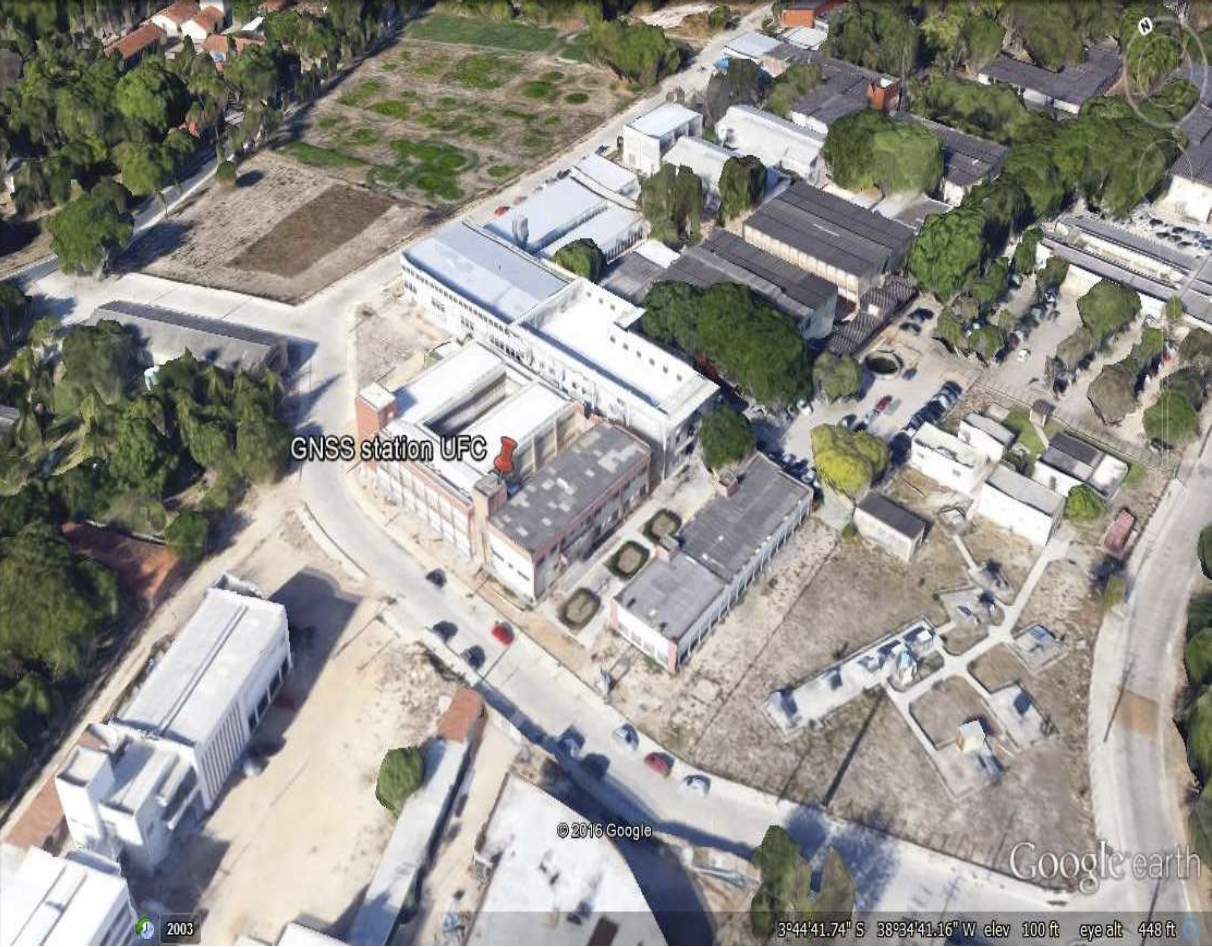
\includegraphics[width=0.7\textwidth]{google_earth_ufc.png}
    \caption{Local da antena GNSS instalada no telhado do prédio do \gls{deti} (imagem: Google Earth).}
    \label{fig:antena}
\end{figure}

\begin{figure}[htbp]
        \centering
        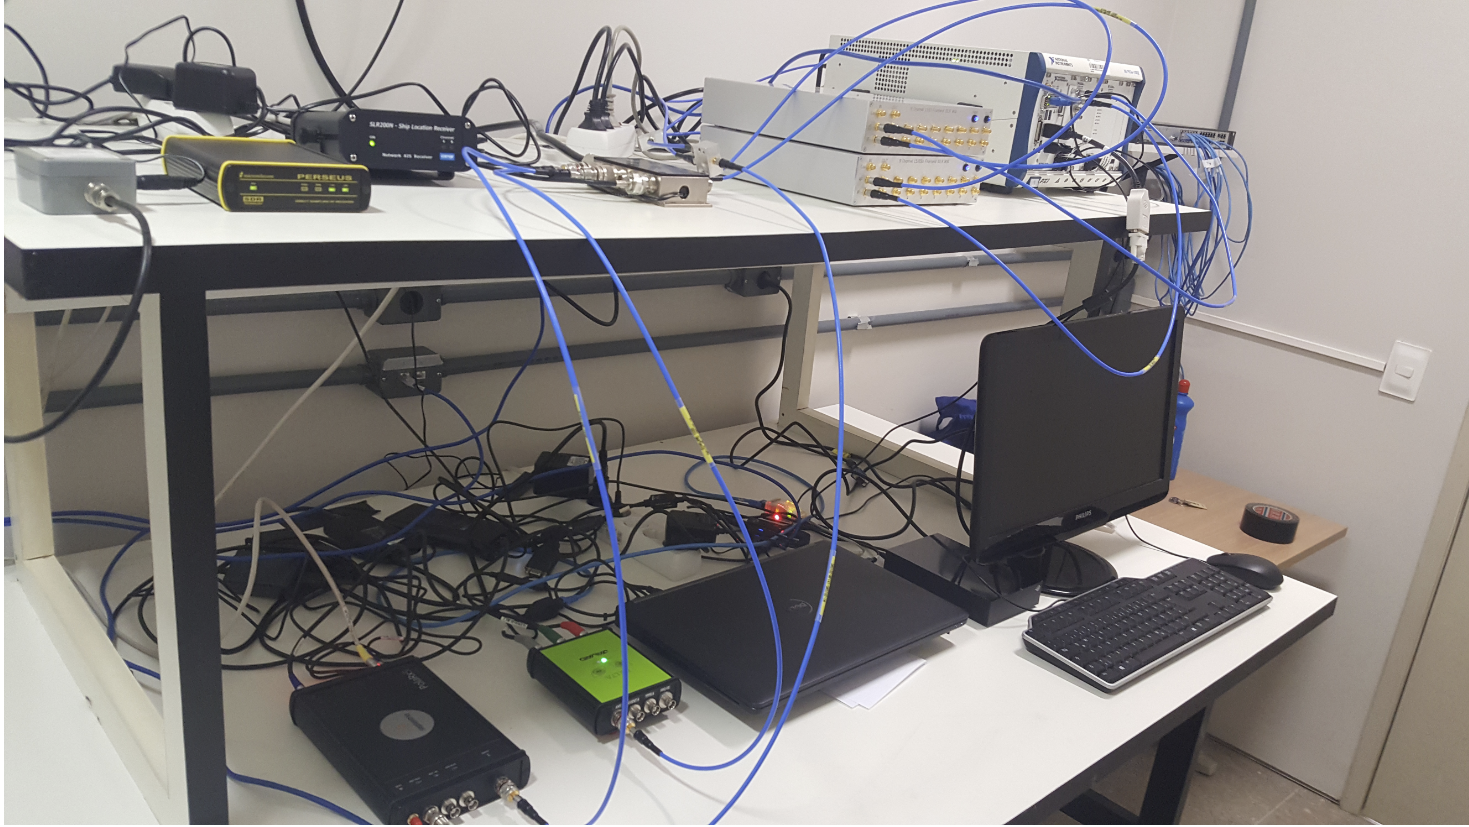
\includegraphics[width=0.8\textwidth]{bancada_do_antigo_lap2se.png}
        \caption{Bancada onde foram instalados os equipamentos do DLR.}
        \label{fig:bancada}
\end{figure}

\begin{figure}[htbp]
    \centering
    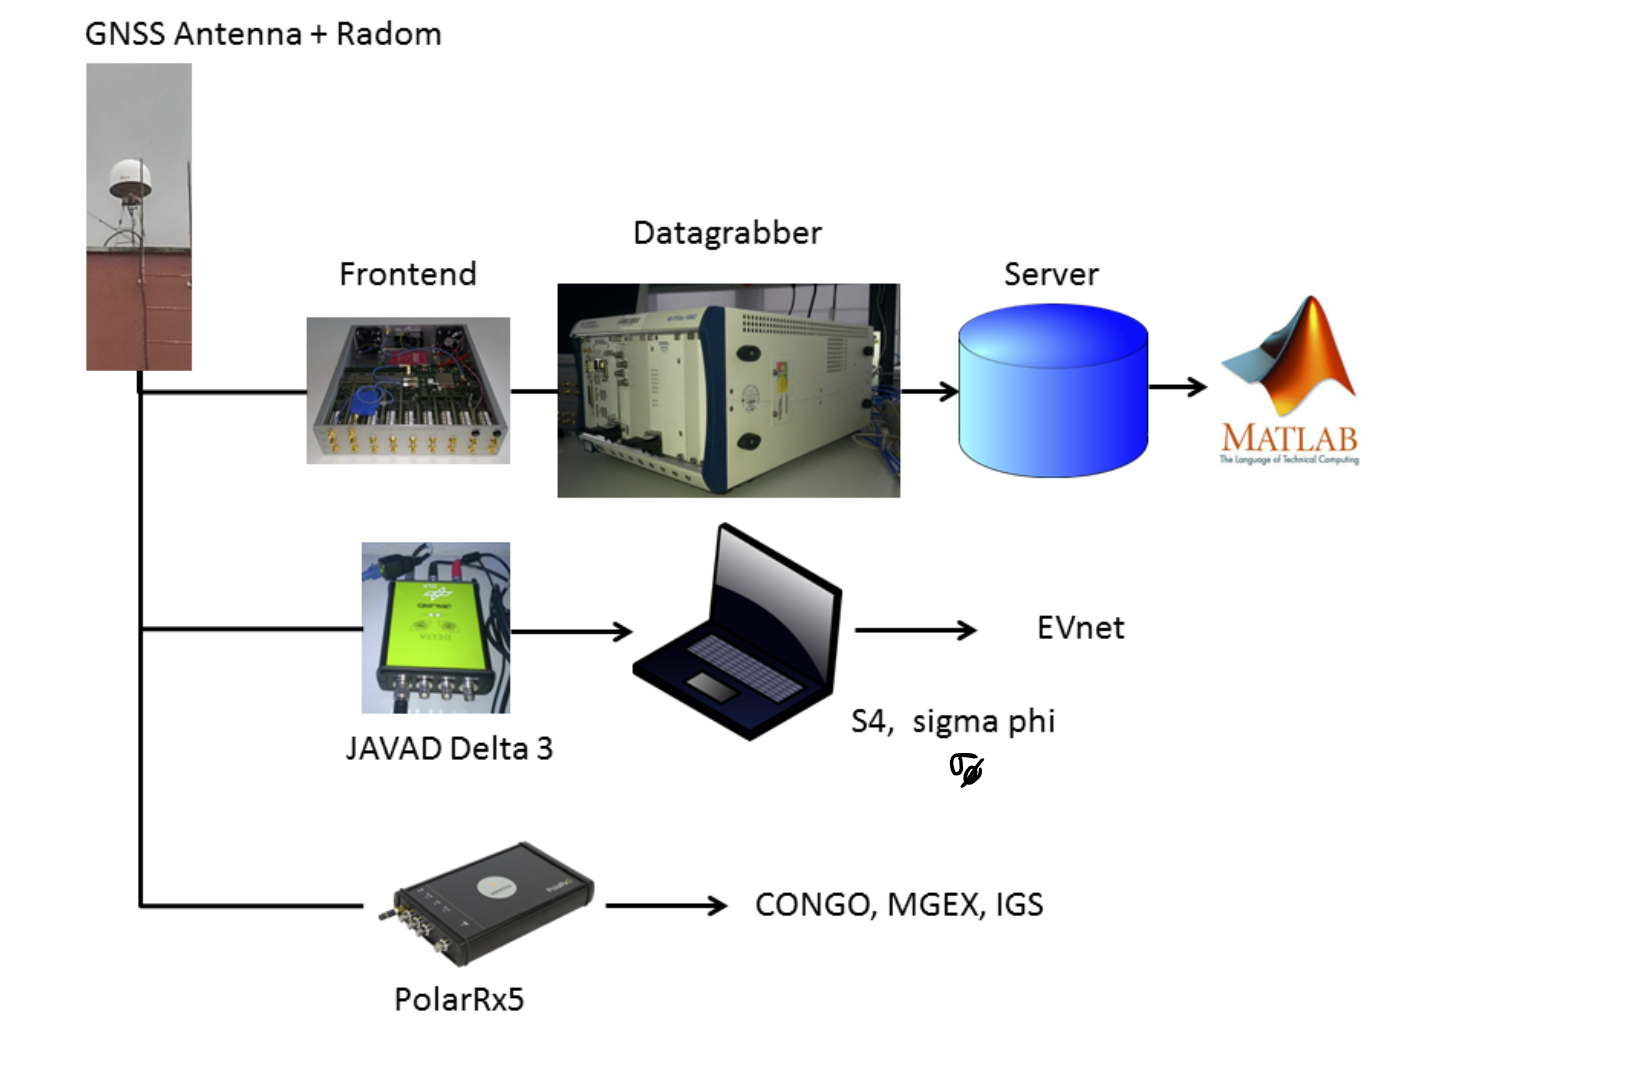
\includegraphics[width=1.2\textwidth]{sistema_de_coleta_lap2se.png}
    \caption{Esquema do sistema de coleta e aquisição de dados utilizado no LAP2SE.}
    \label{fig:coleta}
\end{figure}

\subsection{Doutorado UFC/UPC/ITA: diversificação, internacionalização e produtividade científica}

O ingresso no doutorado do \cgls{ppgeti} em agosto de 2021 ocorreu nesse contexto de consolidação do programa como \cgls{capes} 6, início das pesquisas em \cgls{gnss} e monitoramento da cintilação ionosférica, chegada do Prof. Dr. Felix Dieter Antreich e aposentadoria de alguns colaboradores com quem trabalhei na graduação e no mestrado. Sabia que precisava diversificar e internacionalizar minha atuação no doutorado e, ainda, seguir na área satelital. Das vagas disponibilizadas, somente eu fui aprovado para a linha de pesquisa de monitoramento da cintilação ionosférica a nível de doutorado; as outras vagas não foram preenchidas.

O projeto de doutorado, intitulado "\emph{Ionospheric Scintillation Monitoring with GNSS and Event Classification}", teve como objetivo o desenvolvimento de métodos avançados de processamento de sinais e inteligência artificial para a detecção e caracterização da cintilação ionosférica em regiões equatoriais. O projeto teve como orientador o Prof. Dr. Felix Antreich e como coorientador o Prof. Dr. André Lima Ferrer de Almeida. Apesar dos eventos promissores que antecederam o ingresso no doutorado, um evento crítico ocorreu em 2018: o Prof. Dr. Felix Antreich, então professor visitante na \cgls{ufc}, tornou-se professor efetivo do \cgls{ita}, em São José dos Campos, e não havia outro professor no \cgls{ppgeti} com expertise na área. Devido a isso, o doutorado foi marcado pela pluralidade institucional, com pesquisas e atividades acadêmicas realizadas em várias cidades. Vejo isso como um acaso feliz, pois possibilitou a consolidação de parceiros de trabalho na \cgls{ufc}, na \cgls{upc} e no \cgls{ita}, proporcionando diversificação, internacionalização e maior produtividade científica.

\subsubsection{Período na UFC: diversificação da atuação}

O início do doutorado ocorreu na \cgls{ufc}, onde estudei, de forma independente, a cintilação ionosférica e os sistemas \cgls{gnss}, além de cumprir o ciclo de disciplinas obrigatórias do \cgls{ppgeti}.

Diferentemente do mestrado, no doutorado as disciplinas selecionadas cobriram temas fora do meu rol habitual: houve diversificação de assuntos estudados, embora tangencialmente relacionados à minha área. A partir do trabalho realizado com o Prof. Dr. Nicolas Araújos \cite{moreiraConvolutionalLongShortTermMemory2022} e de estudos sobre aplicações de redes neurais para caracterização e detecção de séries temporais, aprofundei-me em aprendizado de máquina, redes neurais, reconhecimento de padrões e inteligência artificial. Isso permitiu desenvolver habilidades analíticas e de modelagem computacional para construir modelos de aprendizado de máquina voltados à detecção e caracterização de séries temporais, incluindo, potencialmente, as observações das perturbações de amplitude e fase dos sinais \cgls{gnss} causadas pela cintilação ionosférica. Sabia que o forte do \cgls{ppgeti} era o processamento de sinais e a inteligência artificial; portanto, decidi aproveitar o ciclo de disciplinas para fortalecer-me nesse tópico, que no doutorado tinha maior aplicabilidade.

De maneira paralela, dediquei-me a estudar um assunto então pouco explorado por mim: sistemas de navegação global via satélite. De forma autodidata, com indicações de referências do Prof. Dr. Felix Dieter Antreich, estudei os fundamentos dos sistemas de navegação por satélite, como o \gls{gps}, Galileo, \cgls{glonass} e Beidou, o que me permitiu compreender a estrutura dos sinais, os algoritmos de posicionamento e as vulnerabilidades desses sistemas a perturbações ionosféricas. Além disso, o estudo sobre cintilação ionosférica permitiu compreender a fenomenologia do evento e os modelos de referência para a geração de dados sintéticos de cintilação.

\subsubsection{Período na UPC: internacionalização}

Em 2023, ingressei em um doutorado em regime de co-tutela internacional na \cgls{upc}, em Barcelona, Espanha. Obtive uma bolsa de doutorado em co-tutela da Comissão Europeia através do projeto GIC-BR SI2.809402, que me permitiu morar em Barcelona por seis meses. O doutorado na \cgls{upc} teve como orientadora a Prof. Dr. Angela Aragon-Angel, do Departamento de Matemática da \cgls{upc}, e como coorientador o Prof. Dr. Felix Dieter Antreich. Prof. Felix e eu entendemos que a parceria com a \cgls{upc} era (e continua sendo) estratégica devido à expertise em processamento de dados \cgls{gnss}, área complementar ao meu trabalho, mais focado em processamento de sinais. Essa complementaridade advém do fato de que, uma vez transladado o sinal de \cgls{rf} para \cgls{fi} (ou \cgls{bb}) e estimados parâmetros como fase do código, fase da portadora e desvio Doppler, o próximo passo é a obtenção dos \textit{pseudoranges} e a estimação de posicionamento e tempo do receptor. Ao primeiro passo chamamos "processamento de sinais \cgls{gnss}"; ao segundo, "processamento de dados \cgls{gnss}". O grupo \cgls{gage} da \cgls{upc} é referência mundial em processamento de dados \cgls{gnss}, autor de algoritmos modernos de posicionamento como o \textit{fast-PPP} \cite{rovira-garciaFastPrecisePoint2016}. Outro triunfo do grupo é o software de código aberto \textit{GNSS-SDR} \cite{fernandez-pradesGNSSSDROpenSource2011}, um receptor \cgls{gnss} definido por software amplamente usado por pesquisadores e profissionais. O gLAB, também desenvolvido pelo grupo \cgls{gage}, é um simulador multipropósito para processar e analisar dados de \cgls{gnss} e pode validar a performance de posicionamento a partir de sinais corrompidos por cintilação.

Assim, o período na \cgls{upc} foi dedicado ao estudo do processamento de dados \cgls{gnss}. O foco foi: 1) compreender toda a cadeia de processamento de dados \cgls{gnss}; 2) estudar como a cintilação ionosférica afeta o posicionamento do receptor; 3) familiarizar-me com o gLAB e o GNSS-SDR. Durante o período (janeiro–agosto de 2024) escrevi e submeti um artigo para o ION GNSS+2024, intitulado "\emph{Convolutional Neural Networks for Time Series Classification of Ionospheric Scintillation}", aceito para apresentação \cite{pacelliConvolutionalNeuralNetworks2024}, marcando meu primeiro congresso internacional.

\subsubsection{Período no ITA: produtividade científica}

Ao retornar ao Brasil, em agosto de 2024, dirigi-me ao \cgls{ita}, em São José dos Campos, onde o Prof. Dr. Felix Dieter Antreich é professor efetivo. Era o momento de impulsionar minha produtividade científica, e o ambiente do \cgls{ita} ofereceu suporte para isso.

Morei em São José dos Campos por 14 meses, período em que desenvolvi pesquisas com o Prof. Dr. Felix Dieter Antreich e outros pesquisadores do laboratório \cgls{gnss}/\cgls{gps}, como o Msc. Rodrigo Florindo e a Dra. Danielle. Em termos de sinergia, foi no \cgls{ita} que obtive maior colaboração, visto que, na \cgls{ufc}, eu era o único pesquisador do programa com expertise em monitoramento da cintilação ionosférica e processamento de sinais \cgls{gnss}, e na \cgls{upc} estava mais envolvido com estudos e redação de artigos. Foi durante esse período em São Paulo que desenvolvi diversos artigos científicos, incluindo meu primeiro artigo publicado em periódico de alto impacto: o periódico Digital Signal Processing (Elsevier) \cite{pacelliAlldigitalCoherentAFSK2025,pacelliCharacterizationIonosphericScintillation2025,florindoAdvancedKalmanFilter2025}. Há ainda um quarto artigo, também em periódico de alto impacto, em processo de revisão.

Em 2025, participei de um \cgls{ted}, fruto de parceria entre o \cgls{ita} e a \cgls{anatel}. O \cgls{ted} possui vários eixos de desenvolvimento; meu foco foi o eixo quarto: monitoramento espectral, com objetivo de desenvolver um sistema de vigilância autônomo, eficiente e robusto para a detecção, classificação e caracterização de sinais de telecomunicações em faixas regulamentadas pela \cgls{anatel}. Nesse trabalho, aproveitei minha expertise em comunicação digital, processamento de sinais e inteligência artificial para desenvolver um modelo que utiliza espectrogramas coletados in loco por meio de um rádio definido por software. Também revisitei tópicos como sistemas de radiodifusão, radioenlace \cgls{ptp} e comunicações móveis. Estudaram-se esquemas de modulação, multiplexação, codificação e sinais de áudio e vídeo para construir um modelo de detecção, classificação e caracterização de emissores, com aplicação à fiscalização espectral pela \cgls{anatel}.

Recentemente, em abril de 2026, defendi meu doutorado em São José dos Campos, com a tese "\emph{Detection and characterization of equatorial ionospheric scintillation based on GNSS observations using convolutional neural networks}", tanto pela \cgls{ufc} quanto pela \cgls{upc}. A inserção de \cglspl{cnn} para detecção e caracterização de eventos de cintilação ionosférica foi prevista desde o início do doutorado: as CNNs são eficazes na detecção e classificação de padrões em séries temporais, assim como são consagradas em visão computacional \cite{ismailfawazDeepLearningTime2019}.

\subsection{Cenário atual e perspectivas futuras}

Enquanto morei na Europa, em 2024, nasceu na \cgls{ufc} o \cgls{inct} \textit{signals} \cite{andrelimaferrerdealmeidaINCTSignals}. Com foco em sensores ópticos e de \cgls{rf} embarcados em sistemas aerotransportados, como satélites ou veículos autônomos, o \cgls{inct} \textit{signals} tem por objetivo a coleta de dados para observação da Terra, monitoramento de tráfego e segurança nacional, navegação \textit{indoor} e \textit{outdoor}, etc. Trata-se de um \cgls{inct} heterogêneo, com pesquisadores de diversas áreas, mas com foco central em sensoriamento e vigilância remota. O \cgls{inct} \textit{signals} tem sede na \cgls{ufc} e é coordenado pelo Prof. Dr. André Lima Ferrer de Almeida, meu coorientador no doutorado, congregando pesquisadores de instituições como \cgls{unipampa}, \cgls{ufrgs}, \cgls{pucrs} e \cgls{ita}.

É nesse contexto que me situo: sou bolsista de pós-doutorado \gls{dti-a} do \cgls{cnpq}, bolsa proveniente do \cgls{inct} \textit{signals}. Institucionalmente, estou vinculado tanto ao \cgls{ppgeti}/\cgls{ufc} quanto ao \cgls{pgeec}/\cgls{ita}, e trabalho com o Prof. Dr. André Lima Ferrer de Almeida e com o Prof. Dr. Felix Antreich em assuntos relacionados ao \cgls{inct} \textit{signals}.

A curto prazo, meu objetivo no pós-doutorado é desenvolver um rádio definido por software para o monitoramento da cintilação ionosférica utilizando sinais \cgls{gnss}. Esse objetivo está alinhado com minha trajetória acadêmica e com a história de como a comunicação e navegação por satélite se desenvolveram na \cgls{ufc}/\cgls{deti}: os equipamentos do \cgls{dlr} estão instalados no \cgls{deti} desde 2017; o \cgls{dlr} utiliza tais dados, enviados de Fortaleza para a Alemanha por meio de túnel Ethernet sobre IP, mas a \cgls{ufc} ainda não explorou plenamente essas informações. De fato, o que deveria ser um laboratório de monitoramento da cintilação ionosférica no \cgls{deti} é, atualmente, um depósito de materiais onde os equipamentos estão guardados, mas funcionando 24 horas por dia a partir do sinal coletado pela antena instalada no topo do departamento. Desde que parti de Fortaleza em 2024, o \cgls{ppgeti} não gerou recursos humanos com o conhecimento necessário para extrair informações dos sinais \cgls{gnss} coletados, visto que não há pesquisadores com expertise nessa área desde que o Ceará perdeu o Prof. Felix para São Paulo.

Essa realidade muda com meu retorno a Fortaleza e com o fomento do \cgls{inct} \textit{signals}. Se, no doutorado, desenvolvi modelos de inteligência artificial para detecção e caracterização de eventos de cintilação ionosférica a partir de dados sintéticos, no pós-doutorado pretendo desenvolver um rádio definido por software para processar os dados coletados, a fim de extrair o sinal de cintilação ionosférica a partir dos sinais \cgls{gnss} obtidos no laboratório do \cgls{deti}. Isso abre portas para publicações em periódicos de alto impacto, como os da \cgls{ieee}. A principal crítica aos artigos submetidos durante o doutorado era que os algoritmos foram validados com dados sintéticos e não com dados reais; esse cenário muda quando passo a extrair dados diretamente da estação de monitoramento. É importante ressaltar que dados reais de cintilação disponibilizados publicamente não servem para o interesse da pesquisa, pois normalmente armazena-se apenas os índices de cintilação (\(S_4\) e \(\sigma_{\phi}\)), quando o que interessa é a extração do sinal de cintilação ionosférica da saída do pós-correlator, algo que não é feito nas estações de monitoramento tradicionais. Por isso a necessidade da implantação de uma estação própria de monitoramento, que servirá de base para uma nova abordagem de detecção e caracterização de eventos de cintilação ionosférica.

O \cgls{inct} \textit{signals} serve como guarda-chuva institucional e financeiro para essa estação. Além disso, o que era um depósito de materiais deve tornar-se um laboratório de fato, denominado \gls{senselab}. O nome do laboratório indica que, além do monitoramento da cintilação ionosférica, o objetivo a longo prazo é desenvolver algoritmos de processamento de sinais e inteligência artificial para aplicações satelitais, como comunicação e navegação via satélite, sensoriamento remoto e observação da Terra. O laboratório, inicialmente com material cedido pelo \cgls{dlr}, deve passar por reforma e futuramente ser equipado com sistemas computacionais de alto desempenho, como servidores e estações de trabalho, para o desenvolvimento de pesquisas em processamento de sinais e inteligência artificial. A expectativa é inaugurar o laboratório em 2026 e consolidar o monitoramento da cintilação ionosférica como uma das principais linhas de pesquisa.

O rádio definido por software para o monitoramento da cintilação ionosférica utilizando sinais \cgls{gnss} é similar aos receptores tradicionais, como o GNSS-SDR desenvolvido pelo grupo \cgls{gage} da \cgls{upc}, mas será otimizado para a extração do sinal de cintilação ionosférica em vez da extração de pseudoranges para posicionamento. Dessa distinção, decorre a necessidade de desenvolver algoritmos personalizados para o receptor baseado em software. Portanto, o código-fonte do GNSS-SDR (em C++) deve ser utilizado como base, com modificações significativas nos módulos de rastreamento de portadora e código, para otimizar a estimação de parâmetros de fase e amplitude do sinal de cintilação ionosférica. Enquanto o problema de estimação do sinal de cintilação foi desenvolvido em colaboração com o Msc. Rodrigo Florindo \cite{florindoAdvancedKalmanFilter2025}, o problema de detecção e caracterização a partir dos parâmetros de fase e amplitude foi desenvolvido durante o doutorado. Agora, é necessário integrar esses métodos ao receptor baseado em software para construir uma estação de monitoramento que utilize uma nova abordagem de detecção e caracterização.

No entanto, não pretendo dedicar-me exclusivamente a um tema. A médio e longo prazo, pretendo diversificar minha atuação para outras áreas adjacentes à comunicação e navegação por satélite, sempre com foco na cadeia de processamento de sinais e imagens, seja usando métodos clássicos, seja métodos de inteligência artificial. Tópicos como
\begin{itemize}
    \item comunicação e navegação via satélite,
    \item processamento estatístico de sinais e imagens,
    \item \Gls{fpga} e sistemas computacionais microprocessados,
    \item sistemas radioenlace e radiodifusão
\end{itemize}

são de meu interesse. Pretendo aplicar esses conhecimentos em:
\begin{itemize}
    \item sensoriamento remoto,
    \item observação da Terra,
    \item projetos de rádio definido por software em sistemas embarcados para comunicação e navegação robusta e eficiente,
    \item uso de inteligência artificial para sensoriamento espectral: detecção, classificação e caracterização de sinais de radiodifusão, radioenlace \cgls{ptp}, comunicação móvel e outros emissores.
\end{itemize}

Acredito que minha trajetória acadêmica é marcada pela diversificação de temas, conferindo-me um perfil multidisciplinar, ao mesmo tempo unido por um foco central em processamento de sinais e imagens em sistemas de comunicação e navegação via satélite.

% (O restante do documento foi mantido na estrutura original; correções similares foram aplicadas ao longo do texto onde necessário.)

\section{Titulação Acadêmica}

% (Seção mantida; pequenas correções tipográficas aplicadas onde cabível no texto acima.)

\begin{itemize}
  \item \textbf{Doutorado (em regime de cotutela) em Ciência e Tecnologia Aeroespacial}
  \begin{itemize}
    \item Tese: "\emph{Detection and characterization of equatorial ionospheric scintillation based on GNSS observations using convolutional neural\linebreak networks}";
    \item Universidade: \glsentrylong{upc};
    \item Local:  Barcelona, Espanha;
    \item Período: 2023--2026;
    \item Programa: Post-graduate program in Aerospace Science and Technology.
    \item Grupo de pesquisa: \glsentrylong{gage}.
    \item Orientador: Prof. Dr. Angela Aragon-Angel (\glsentrylong{upc});
    \item Coorientador: Prof. Dr. Felix Dieter Antreich (\glsentrylong{ita});
  \end{itemize}
  %
  \item \textbf{Doutorado em Engenharia de Teleinformática}
  \begin{itemize}
    \item Tese: "\emph{Detection and characterization of equatorial ionospheric scintillation based on GNSS observations using convolutional neural\linebreak networks}";
    \item Universidade: \glsentrylong{ufc};
    \item Local: Fortaleza, CE, Brasil;
    \item Período: 2021--2026;
    \item Programa: \glsentrylong{ppgeti};
    \item Grupo de pesquisa: \glsentrylong{lasp}.
    \item Orientador: Prof. Dr. Felix Dieter Antreich (\glsentrylong{ita}), 
    \item Co-orientador: Prof. André Lima Ferrer de Almeida (\glsentrylong{ufc}).
  \end{itemize}
  %
  \item \textbf{Mestrado em Engenharia de Teleinformática}
  \begin{itemize}
    \item Dissertação: "\emph{Modem AFSK Coerente e Completamente Digital para Módulo TT\&C Padrão CubeSat}";
    \item Universidade: \glsentrylong{ufc};
    \item Local: Fortaleza, CE, Brasil;
    \item Período: 2019--2021;
    \item Programa: \glsentrylong{ppgeti};
    \item Orientador: Prof. Dr. João Cesar Moura Mota (aposentado pela \glsentrylong{ufc});
    \item Coorientador: Prof. Dr. Antônio Macilio Pereira de Lucena (aposentado pelo \glsentrylong{inpe}).
  \end{itemize}
  %
  \item \textbf{Graduação em Engenharia Eletrônica}
  \begin{itemize}
    \item Trabalho de conclusão de curso: "\emph{Projeto de um conversor para carregador portátil com interface USB tipo-C}";
    \item Universidade: \glsentrylong{unifor};
    \item Local: Fortaleza, CE, Brasil;
    \item Período: 2014--2018;
    \item Curso: Engenharia Eletrônica;
    \item Orientador: Prof. Bruno Ricardo de Almeida (\glsentrylong{unifor}).
  \end{itemize}
\end{itemize}

\section{Atividades de Pesquisa e Produção Científica}

% Lista de publicações mantida; formatação e títulos revisados.

\begin{itemize}
    \item Pacelli, Rubem Vasconcelos, Rodrigo de Lima Florindo, Felix Antreich, André Lima Ferrer de Almeida, Angela Aragon-Angel, and Adrià Rovira Garcia. “Characterization of Ionospheric Scintillation Using Deep Learning Models.” September 12, 2025, 3339–52. \url{https://doi.org/10.33012/2025.20390}.
    \item Pacelli, Rubem Vasconcelos, Rodrigo de Lima Florindo, Felix Antreich, and Antônio Macilio Pereira de Lucena. “An All-Digital Coherent AFSK Demodulator for CubeSat Applications.” Digital Signal Processing 162 (July 2025): 105147. \url{https://doi.org/10.1016/j.dsp.2025.105147}.
    \item Pacelli, Rubem Vasconcelos, Antonio Macilio Pereira de Lucena, and João Cesar Moura Mota. “All-Digital AFSK Modem with Viterbi Detection for TT\&C CubeSat Transceiver.” XXXVIII Simpósio Brasileiro de Telecomunicações e Processamento de Sinais, 2020. \url{https://doi.org/10.14209/SBRT.2020.1570654898}.
    \item Pacelli, Rubem Vasconcelos, Angela Aragon-Angel, Adrià Rovira García, Andre Lima Ferrer de Almeida, and Felix Antreich. “Convolutional Neural Networks for Time Series Classification of Ionospheric Scintillation.” September 19, 2024, 3019–28. \url{https://doi.org/10.33012/2024.19929}.
    \item Pacelli, Rubem V., Nícolas De A. Moreira, Tarcisio F. Maciel, Modeste Kacou, and Marielle Gosset. “A Data-Based Estimation of Power-Law Coefficients for Rainfall via Levenberg-Marquardt Algorithm: Results from the West African Testbed.” In Proceedings of the 6th International Symposium on Uncertainty Quantification and Stochastic Modelling, edited by José Eduardo Souza De Cursi. Lecture Notes in Mechanical Engineering. Springer International Publishing, 2024. \url{https://doi.org/10.1007/978-3-031-47036-3\_17}.
    \item Moreira, Nícolas de Araújo, Rubem Vasconcelos Pacelli, Yuri Carvalho Barbosa Silva, et al. “Convolutional Long-Short-Term Memory Networks (ConvLSTM) for Weather Prediction Using Radar and Satellite Images.” Congresso Brasileiro de Automática - CBA 3, no. 1 (2022). \url{https://doi.org/10.20906/CBA2022/3299}.
    \item Florindo, Rodrigo de Lima, Rubem Pacelli, Thiago Lobo Ferreira, Daniele Oliveira Silva, Antonio Macilio Pereira de Lucena, and Felix Antreich. “Advanced Kalman Filter Carrier Tracking: Performance Assessment Under Two Ionospheric Scintillation Models.” September 12, 2025, 3421–35. \url{https://doi.org/10.33012/2025.20395}.
\end{itemize}

\section{Atividades de Ensino}

\begin{itemize}
    \item Apoio à disciplina ``Processamento Digital de Sinais'', ministrada pelo Prof. Dr. André Lima Ferrer de Almeida, no \cgls{ppgeti}/\cgls{ufc}, durante o meu mestrado, no período de 2019 a 2021;
    \item Apoio à disciplina ``Sistemas de Comunicações Digitais'', ministrada pelo Prof. Dr. André Lima Ferrer de Almeida, no \cgls{ppgeti}/\cgls{ufc}, durante o meu doutorado, no período de 2021 a 2024;
\end{itemize}

\section{Extensão e inovação}

\begin{itemize}
    \item Desenvolvimento da patente BR 10 2021 023220 0 A2, ``ARQUITETURA DE DEMODULAÇÃO DIGITAL E MÉTODO DE DETECÇÃO COERENTE PARA SINAIS AFSK'', depositada em 2021, com o objetivo de proteger a arquitetura de demodulação digital e método de detecção coerente para sinais AFSK, que foi desenvolvida durante o meu mestrado e publicada em um artigo de periódico de alto impacto \cite{pacelliAlldigitalCoherentAFSK2025}.
    \item Desenvolvimento de um sistema de vigilância espectral para a detecção, classificação e caracterização de sinais de telecomunicações utilizando inteligência artificial, em parceria com o \cgls{ita} e a \cgls{anatel}, como parte do eixo quarto do \cgls{ted} entre o \cgls{ita} e a \cgls{anatel}.
\end{itemize}


\part{Projeto de Atuação Profissional - PAP}

\section{Introdução}

O objetivo dessa seção é apresentar os pressupostos teóricos que fundamentam o \cgls{pap} que proponho para a \cgls{ufrn}. Para isso, relaciono o presente \cgls{pap} e minha trajetória acadêmica-profissional (descrita na Parte~\ref{part:memorial}) com a área de conhecimento objeto do concurso e com a expectativa de atuação profissional da vaga 694958, ``Radiodifusão Digital e Sistemas de Comunicações via Satélite'', em todos os âmbitos do magistério superior: ensino, pesquisa, extensão e inovação.

O \cgls{pap} que proponho para a \cgls{ufrn} está diretamente alinhado com a minha trajetória acadêmica e com o meu objetivo de longo prazo, que é ser um pesquisador e professor universitário na área de comunicação e navegação via satélite, com foco em processamento de sinais/imagens e inteligência artificial. A fim de elaborar uma plano atuação abrangente e que atenda às demandas internas a externas da \cgls{ufrn}, faz-se necessário: 1) análise institucional da \cgls{ufrn}, do \gls{cetel} e do \cgls{ppgeec}; 2) compreender o cenário socio-econômico-industrial do estado do Rio Grande do Norte, do Nordeste, e do Brasil. Essa análise está sintetizada no quadro \cgls{fofa} apresentado na Tabela~\ref{tab:quadro-fofa}, que é a base para a definição dos objetivos do meu \cgls{pap}.

\begin{table}[htbp]
  \centering
  \caption{Quadro \gls{fofa} — \gls{ufrn} / \gls{cetel} / \gls{ppgeec}}
  \label{tab:quadro-fofa}
  \begin{tabular}{|p{0.5\textwidth}|p{0.58\textwidth}|}
    \hline
    \textbf{Forças} (interno) & \textbf{Oportunidades} (externo) \\
    \hline
    \begin{enumerate}[label=F\arabic*]\vspace{0pt}\item \textbf{Universidade com caráter tecnológico}: líder em inovação na região Nordeste devido ao seu alto volume de concessões de patentes nas regiões Norte, Nordeste e Centro-Oeste \cite{oliveira2025_evasao}. \item \textbf{Infraestrutura de laboratórios modernos}: mais de R\$ 1 milhão investidos em laboratórios especializados, como o de Convergência de Redes (LABCONVEX), Simulação e Prototipagem (LabSim), Radiofrequência (LABRF) e Comunicações Ópticas \cite{NovosLaboratoriosImpulsionam}. \end{enumerate}
    &
    \begin{enumerate}[label=O\arabic*]\vspace{0pt}\item \textbf{RN como polo estratégico espacial e de defesa}: A proximidade com o Centro de Lançamento da Barreira do Inferno e propostas de parceria com a \cgls{aeb} e o \cgls{inpe} abrem frentes de trabalho únicas na região \cite{ufrn_ppc_telecom_2024} \item \textbf{Mercado global e nacional em expansão}: Há uma projeção de 90 milhões de empregos globais em Tecnologias de Informação e Comunicação (TIC) até 2025, com um crescimento médio de 8\% a 15\% na contratação de engenheiros no Rio Grande do Norte \cite{cetel_carreira} \end{enumerate} \\
    \hline
    \textbf{Fraquezas} (interno) & \textbf{Ameaças} (externo) \\
    \hline
    \begin{enumerate}[label=f\arabic*]\vspace{0pt}\item \textbf{Altas taxas de evasão}: O curso enfrenta dificuldades históricas com a retenção de alunos (reprovações frequentes em determinados componentes curriculares) e a evasão frequente de estudantes \cite{ufrn_resolucao_sipac} \item \textbf{Orientação acadêmica insuficiente}: Diagnósticos internos apontaram um baixo índice de orientação acadêmica cadastrada e a necessidade de maior envolvimento do corpo docente na mentoria dos alunos \cite{ufrn_resolucao_sipac} \end{enumerate}
    &
    \begin{enumerate}[label=A\arabic*]\vspace{0pt}\item \textbf{Restrições orçamentárias e humanas no setor espacial}: Limitações de orçamento dificultam a manutenção e investimento em infraestruturas e tecnologias essenciais. Há também carência de colaboradores (servidores efetivos), o que sobrecarrega a equipe e reduz a velocidade de entregas \cite{aeb_relatorio_gestao_2025} \item \textbf{Baixa complexidade da cadeia industrial do setor produtivo nordestino e sua desconexão com a academia}:  as exportações nordestinas representam menos de 10 \% do total das exportações brasileiras e concentram-se em \textit{commodities} e produtos intermediários ou semimanufaturados \cite{ipea_240_1}. Em contraste, a Academia tende a (e deve) focar em pesquisas de ponta, mas a falta de conexão com o setor produtivo local dificulta a transferência de conhecimento e tecnologia para a região. \end{enumerate} \\
    \hline
  \end{tabular}
\end{table}

\section{Objetivos}
\label{sec:objetivos}

Dado o atual cenário socio-econômico-industrial do estado do Rio Grande do Norte, do Nordeste e do Brasil, e considerando as forças, fraquezas, oportunidades e ameaças apresentadas na Tabela~\ref{tab:quadro-fofa}, os objetivos do meu \cgls{pap} são os seguintes:

\textbf{Objetivo geral}
\begin{itemize}
    \item Contribuir para o desenvolvimento da \cgls{ufrn} como um centro de excelência no que tange a pesquisa, ensino e de desenvolvimento tecnológico em comunicação e navegação via satélite, com foco em processamento de sinais/imagens e inteligência artificial, alinhado com as necessidades do setor aeroespacial e de defesa do Rio Grande do Norte, do Nordeste e do Brasil.
\end{itemize}


\textbf{Objetivos específicos}:
  \begin{enumerate}[label=e\arabic*.]
    \item Desenvolver pesquisas de alto impacto científico a fim de aumentar a \textbf{produção científica} da \cgls{ufrn} e do \cgls{ppgeec}, sempre com o foco no aumento da nota \cgls{capes} do programa;
    \item Competir por \textbf{recursos financeiros} de agências de fomento nacionais e internacionais para o desenvolvimento de pesquisas e projetos de interesse do \cgls{ppgeec}, sempre levando o contexto tecnológico do estado do Rio Grande do Norte e os agentes públicos e privados em torno da \cgls{ufrn};
    \item Desenvolver \textbf{patentes} e inovações tecnológicas que possam ser transferidas para o setor produtivo, especialmente para o setor aeroespacial e de defesa, na área de comunicação e navegação, a fim de aumentar a relevância social da \cgls{ufrn} e do \cgls{ppgeec};
    \item Buscar \textbf{conectar a pesquisa acadêmica com as necessidades do setor produtivo}, o que pode ser feito diretamente com empresas via parceria pública (\gls{ufrn}) e privada (setor produtivo), por intermédio de agências de fomento governamentais, ou por meio de incubadoras e parques tecnológicos;
    \item Usar minha expertise em comunicação e navegação via satélite para construir uma \textbf{estação de coleta de dados} satelitais, e a partir disso, desenvolver pesquisas e projetos relacionados a processamento de sinais/imagens e inteligência artificial;
    \item Manter \textbf{parcerias} entre outras universidades e instituições de pesquisa e ensino superior, tanto nacionais quanto internacionais, para o desenvolvimento de pesquisas e projetos de interesse do \cgls{ppgeec};
    \item Desenvolver \textbf{projetos de ensino} relacionados a comunicação e navegação via satélite, processamento de sinais/imagens e inteligência artificial, e lecionar disciplinas obrigatórias e optativas relacionadas a esses temas no \cgls{cetel} e no \cgls{ppgeec}, tanto na graduação quanto na pós-graduação;
    \item Gerar \textbf{recursos humanos} qualificados em pesquisas a nível de graduação, e por meio de atividades orientações de trabalhos de conclusão de curso e de iniciação científica, e a nível de pós-graduação, por meio de orientações de mestrado e doutorado;
  \end{enumerate}


Até o fim deste documento, explana-se um plano de ação para alcançar os objetivos propostos nesta Seção. As atividades aqui apresentadas perpassam por todas as áreas de atuação do magistério, isto é, ensino, pesquisa, extensão e gestão.

\section{Atividades de ensino}

A Tabela~\ref{tab:disciplinas-uern} apresenta o rol de disciplinas da \cgls{ufrn} que estou apto a lecionar, considerando nesta subseção apenas as disciplinas de graduação. As disciplinas aqui listadas são as mesmas daquelas listadas no documento denominado ``Programa, relação de temas da didática e expectativa de atuação profissional'', disponibilizado para os candidatos ao processo seletivo.

\begin{table}[H]
  \centering
  \caption{Rol de disciplinas da UFRN que estou apto a lecionar da Graduação}
  \label{tab:disciplinas-uern}
  \begin{tabular}{|p{0.14\textwidth}|p{0.18\textwidth}|p{0.44\textwidth}|p{0.16\textwidth}|}
    \hline
    \textbf{Nível} & \textbf{Código} & \textbf{Nome} & \textbf{Observações} \\
    \hline
    Graduação & DCO3003 & Análise e Síntese de Circuitos Elétricos & Obrigatória \\
    \hline
    Graduação & DCO3005 & Variáveis Aleatórias & Obrigatória \\
    \hline
    Graduação & DCO3007 & Circuitos Digitais Combinacionais & Obrigatória \\
    \hline
    Graduação & DCO3008 & Princípios de Telecomunicações & Obrigatória \\
    \hline
    Graduação & DCO3010 & Dispositivos Eletrônicos & Obrigatória \\
    \hline
    Graduação & DCO3014 & Comunicações Digitais & Obrigatória \\
    \hline
    Graduação & DCO3016 & Sistemas Digitais & Obrigatória \\
    \hline
    Graduação & DCO3017 & Circuitos para Comunicações & Obrigatória \\
    \hline
    Graduação & DCO3020 & Propagação & Obrigatória \\
    \hline
    Graduação & DCO3022 & Sistemas de Telecomunicações & Obrigatória \\
    \hline
    Graduação & DCO3027 & Comunicações sem Fio & Obrigatória \\
    \hline
    Graduação & DCO3030 & Comunicações Móveis & Obrigatória \\
    \hline
    Graduação & DCO1025 & Processos Estocásticos & Optativa \\
    \hline
    Graduação & DCO1027 & Televisão Digital & Optativa \\
    \hline
    Graduação & DCO1033 & Sistemas de Comunicações via Satélite & Optativa \\
    \hline
    Graduação & DCO1034 & Infraestrutura para Telecomunicações & Optativa \\
    \hline
    Graduação & DCO2007 & Laboratório de TV Digital & Optativa \\
    \hline
    % Pós-graduação & PPGEEC2317 & Sistemas Probabilísticos & Componente básica \\
    % \hline
    % Pós-graduação & PPGEEC2333 & Comunicações Móveis & Componente básica \\
    % \hline
    % Pós-graduação & PPGEEC2336 & Comunicações sem Fio & Componente específica \\
    % \hline
    % Pós-graduação & PPGEEC2337 & Radiopropagação & Componente específica \\
    % \hline
    % Pós-graduação & PPGEEC2340 & Tópicos Especiais em Sistemas de Telecomunicações & Tópicos especiais \\
    % \hline
  \end{tabular}
\end{table}

Para essas disciplinas, detalha-se a seguir o plano de ensino, incluindo a metodologia, métodos de avaliação, e outras informações relevantes para a condução das atividades de ensino.

\subsection{Metodologia de ensino}

A metodologia de ensino que pretendo adotar segue, fundamentalmente, duas filosofias de aprendizagens complementares:
\begin{itemize}
	\item aprendizado baseado em problema (\textit{problem-based learning});
	\item aprendizado pela prática (\textit{learning by doing}).
\end{itemize}

A nível de graduação, essas abordagens são direcionadas para a resolução de problemas de interesses industriais e mercadológicos. Em cada disciplina, os alunos serão desafiados a resolver um problema prático relacionado ao conteúdo teórico lecionado em sala de aula. A depender do tema da disciplina, os alunos podem desenvolvê-la individualmente ou em grupos, e podem ser incentivados a usar ferramentas digitais de desenvolvimento, software de simulação, linguagens de programação, e outras tecnologias digitais que sejam relevantes para a resolução do problema proposto. O objetivo é que os alunos possam aplicar os conceitos teóricos aprendidos em sala de aula para resolver problemas reais, o que pode aumentar a motivação e o engajamento dos alunos, além de prepará-los melhor para o mercado de trabalho.

Ainda sobre o conceito de metodologia de ensino, aplico mais dois conceitos, que os chamo de ``proporcionalidade'' e ``compatibilidade''. O primeiro se refere à ideia de que o nível da complexidade dos problemas propostos deve ser proporcional ao nível de conhecimento e habilidade do professor e à porcentagem de conhecimento transmitido ao aluno. O segundo se refere à ideia de que o nível da complexidade dos problemas propostos deve ser compatível com 1) o nível do aluno; 2) o semestre em que a disciplina é lecionada; 3) o nível (obrigatória ou optativa) e carga horária da disciplina. A ideia é que, conjuntamente, essas metodologias de ensino possam mitigar a grande evasão que o \gls{cetel} enfrenta.


\subsection{Projetos e versionamento de código}

Ressalta-se que a abordagem de \textit{problem-based learning} é fortemente guiada pelos conceitos de versionamento de código, estruturação de projetos de hardware, software e firmware, rastreabilidade de experimentos, e automação de processos de desenvolvimento, o que é algo que eu já aplico em meus projetos de pesquisa e desenvolvimento, e que pretendo aplicar também em atividades de ensino.

Existe hoje, mais do que nunca, uma grande variedade de tecnologias digitais que facilitam, automatizam, versionam e organizam o processo de desenvolvimento de Engenharia de diversas áreas, incluindo a área de Telecomunicações \cite{deng2026untangling}. Enxergar essa demanda de mercado e usá-la como base estruturante numa abordagem \textit{learning by doing} viabiliza a construção de um ambiente de ensino mais moderno, eficiente e alinhado com as necessidades do mercado de trabalho atual.

Ferramentas como GitHub, GitLab, Bitbucket, e outras plataformas de hospedagem de código fonte, são essenciais para o desenvolvimento de projetos de Engenharia, pois permitem o versionamento de código fonte, a colaboração entre equipes, a rastreabilidade de mudanças, e a automação de processos de desenvolvimento. Além disso, ferramentas de integração contínua e entrega contínua (CI/CD) permitem a automação de testes e a entrega rápida de software, o que é fundamental para o desenvolvimento ágil e eficiente \cite{deng2026untangling}. Portanto, acredito que a adoção dessas tecnologias digitais no processo de ensino é essencial para preparar os alunos para o mercado de trabalho atual e futuro.

Infelizmente, engenheiros recém-graduados saem de muitas universidades brasileiras sem o conhecimento de tais ferramentas por simplesmente não exercitá-las durante a graduação, como se não fizesse parte do processo de desenvolvimento de Engenharia \cite{desa2023explorando}. Essa disparidade pode ser parcialmente explicada pelo recente surgimento dessas tecnologias digitais e rápida adoção por parte do mercado de trabalho. Por exemplo, Git, uma das ferramentas de versionamento de código mais populares, foi lançada em 2005 por Linus Torvalds para o desenvolvimento do kernel Linux \cite{northcutt2023evolution}. Depois de um início de adoção lenta (2005--2009), Git cresceu vertiginosamente entre 2010 e 2014 \cite{hecht2020brief}, se tornando a ferramenta de versionamento de código padrão, e muitas vezes, obrigatória na indústria. A rápida adoção de tais ferramentas no mercado de trabalho causou um descompasso entre o ensino e a indústria, algo que deve ser corrigido para preparar os alunos para o mercado de trabalho atual e futuro.

É importante acrescentar que o estímulo do uso dessas ferramentas é ortogonal ao conhecimento teórico lecionado em sala de aula, isto é, pode ser aplicada em qualquer disciplina que tenha um projeto de Engenharia associado, sem qualquer dano quanto à dimensão teórica da disciplina. Por exemplo, em uma disciplina de Comunicações Digitais, os alunos podem ser incentivados a usar o GitHub para versionar o código fonte dos seus projetos de modulação e demodulação digital, enquanto aprendem os conceitos teóricos de modulação e demodulação digital. A vantagem da adição desta dimensão no processo de aprendizagem está no próprio objetivo da ferramenta. Neste exemplo, o aluno poderia retroceder no tempo para recuperar uma versão anterior do código fonte, caso algo dê errado, ou para comparar a evolução do código fonte ao longo do tempo. Além disso, o uso de plataformas de hospedagem de código fonte permite a colaboração entre alunos, o que pode ser benéfico para o processo de aprendizagem, especialmente em projetos de Engenharia que exigem trabalho em equipe.

\subsection{Linguagens de programação priorizadas}

Busco priorizar o ensino de linguagens de programação que sejam amplamente utilizadas na indústria, sobretudo em projetos de Engenharia de Telecomunicações. Devido a heterogeneidade de aplicações demandadas pelo mercado de trabalho de \gls{tic}, e considerando as disciplinas na Tabela~\ref{tab:disciplinas-uern}, as linguagens de programação que pretendo priorizar podem ser categorizadas como segue:
\begin{itemize}
    \item \textbf{Linguagens de baixo nível}: C, C++, Rust, Assembly. Essas linguagens são essenciais para o desenvolvimento de código de baixo nível, como firmware para sistemas embarcados, drivers de dispositivos, e aplicações de tempo real, que são comuns em projetos de eletrônica e telecomunicações.
    \item \textbf{Linguagens de alto nível}: Python, MATLAB e Julia. Essas linguagens são amplamente utilizadas para o desenvolvimento de software de alto nível, como scripts de automação, análise de dados, e desenvolvimento de algoritmos, que são comuns em projetos de processamento de sinais/imagens e inteligência artificial.
\end{itemize}

\subsection{Critério de avaliação}

O critério de avaliação será baseado em uma combinação de fatores, incluindo a qualidade do trabalho entregue, a participação em sala de aula, a capacidade de aplicar os conceitos teóricos para resolver problemas práticos, e o uso efetivo das tecnologias digitais no processo de desenvolvimento dos projetos. A avaliação será contínua ao longo do semestre, com feedback regular para os alunos, a fim de ajudá-los a melhorar seu desempenho e alcançar os objetivos de aprendizagem da disciplina. É importante ressaltar que o critério de avaliação adotado por mim deverá ser alinhado com o componente curricular de cada disciplina \cite{ufrn_ppc_telecom_2024}.

\subsection{Material usado em sala de aula}

Um dos maiores desafios do ensino de Engenharia de Telecomunicações é a abstração dos conceitos teóricos, que muitas vezes são difíceis de entender para os alunos quando não apresentadas de maneiras visual. Para mitigar esse desafio, a abordagem mais comum é a apresentação de slides com eventuais imagens e diagramas, o que pode ser útil para elucidar alguns conceitos.

No entanto, determinados conceitos não podem ser bem elucidados com imagens estáticas, e exigem a apresentação de animações, e por algumas vezes, interações com o usuário/aluno. Para as disciplinas cujo a compreensão se mostra mais difícil, pretendo usar Manim \cite{zhang2025manimstemeducationvisualizing}, uma ferramenta de código aberto para a criação de animações matemáticas, que pode ser usada para criar animações interativas e visualizações de conceitos teóricos complexos, o que pode ajudar os alunos a entender melhor os conceitos teóricos e aumentar o engajamento em sala de aula. Conceitos abstratos, como a transformada de Fourier, a convolução, álgebra linear, entre outros, podem ser melhor elucidados com animações interativas, o que pode facilitar a compreensão dos alunos e aumentar o engajamento em sala de aula \cite{fiori2025objetos}.

\subsection{Propostas de projetos e ferramentas por disciplina}

Propõe-se a seguir um projeto prático para as disciplinas de graduação listadas na Tabela~\ref{tab:disciplinas-uern} para as quais o aprendizado baseado em problema seja aplicável. Além disso, são listadas as ferramentas que os alunos podem usar, seja para o desenvolvimento do projeto, seja para a disciplina como um todo. Os projetos e as ferramentas mencionados a seguir são sugestões que podem ser adaptadas e que buscam estar alinhados com o projeto pedagógico do \cgls{cetel} da \cgls{ufrn} \cite{ufrn_ppc_telecom_2024}, e são baseados na minha experiência acadêmica universitária, bem como na minha experiência em projetos de telecomunicações. Para evitar redundância, evita-se a repetição do conteúdo teórico e as referências bibliográficas, que podem ser consultadas na ementa e bibliografia de cada disciplina em \cite{ufrn_ppc_telecom_2024}, respectivamente. Não obstante, eventuais comentários e referências bibliográficas adicionais são apresentados ao longo da descrição de cada disciplina.


\begin{itemize}
    \item DCO3007 --- Circuitos Digitais Combinacionais:
    \begin{itemize}
        \item \textbf{Observações gerais}: disciplina com carga horária de 15 horas de aulas práticas.
        \item \textbf{Aspectos teóricos}: Para boa parte dos assuntos da ementa\footnote{Introdução aos Circuitos Digitais. Sistemas de Numeração e Códigos Numéricos. Álgebra Booleana. Funções e Portas Lógicas. Análise, síntese e otimização de circuitos combinacionais. Aritmética digital: operações e circuitos. Blocos Operacionais: Contadores, Registradores, Multiplexadores, Demultiplexadores.}, costumo seguir conjuntamente o livro do \cite{tocciDigitalSystems2017} e do \cite{vahidDigitalDesignRTL2010}. Para \gls{hdl}, sigo o livro do \textcite{amoreVHDLDescricaoSintese2012} se o que se deseja for \gls{vhdl}. Se for Verilog, tenho preferência pelo livro do \textcite{chuFPGAPrototypingVerilog2008}.  Eventualmente, trago conteúdos do livro do \textcite{hillArtElectronics2024}, um clássico da área de eletrônica de uma maneira geral.
        \item \textbf{Proposta de projeto}: um projeto prático clássico de circuitos combinacionais a nível de graduação é a criação de um decisor puramente combinacional que, partir de entradas (codificadas) dadas pelo aluno, decide se libera a entrada, calcula uma tarifa/código de cobrança e mostra uma mensagem em display de 7 segmentos. Desenvolvi este mesmo projeto durante a minha graduação, e é um projeto que pode ser adaptado para diferentes níveis de complexidade, dependendo do semestre em que a disciplina é lecionada.
        \item \textbf{Ferramenta}: Além de laboratórios, que costuma ser a forma mais tradicional de ensino de circuitos digitais, pode-se usar ferramentas de simulação digital, como o \textit{Logisim Evolution} \cite{burchLogisimevolution2024}, que é um software de código aberto, gratuito e multiplataforma para o design e simulação de circuitos digitais, que suporta tanto circuitos combinacionais quanto sequenciais, e pode ser usado para o desenvolvimento de projetos práticos em circuitos digitais.
    \end{itemize}
    \item DCO3008 --- Princípios de Telecomunicações:
    \begin{itemize}
        \item \textbf{Observações gerais}: disciplina sem carga horária de aulas práticas.
        \item \textbf{Aspectos teóricos}: normalmente, eu sigo apenas o livro do \textcite{haykinIntroductionAnalogDigital2006}. Entre as disciplinas, com o intuito de compensar o aspecto demasiadamente abstrato de sistemas de comunicações, costumo trazer \textit{datasheets} de transmissores ou receptores reais a nível sistemático, \textit{i.e.}, em forma de diagrama de blocos, para que os alunos possam entender como os conceitos teóricos se aplicam em sistemas reais.
    \end{itemize}
    \item DCO3010 --- Dispositivos Eletrônicos:
    \item \textbf{Observações gerais}: disciplina sem carga horária de aulas práticas.
    \item \textbf{Aspectos teóricos}: no que tange ao estudo de eletrônica de estado sólido, com ênfase nos princípios físicos de dispositivos semicondutores, tenho preferência pelo livro do \textcite{sedraMicroelectronicCircuits2019}. Para análise a nível de sinais e sistemas, como a análise de pequenos sinais em circuitos transistorizados, normalmente migro para o livro do \textcite{boylestadElectronicDevicesCircuit2014}. Normalmente, essa é uma disciplina que observo que os alunos têm mais dificuldade. Quando este é o caso, sigo totalmente o livro do \textcite{boylestadElectronicDevicesCircuit2014}, que tem uma abordagem mais simplificada. Eventualmente, trago conteúdos do livro do \textcite{hillArtElectronics2024}, um clássico da área de eletrônica de uma maneira geral.
    \item DCO3014 --- Comunicações Digitais:
    \item \textbf{Observações gerais}: disciplina sem carga horária de aulas práticas.
    \item \textbf{Aspectos teóricos}: não há uma única referência que eu siga para os conteúdos teóricos previstos na ementa da disciplina. Como aluno, eu segui o livro do \textcite{proakisDigitalCommunications2007}, que é um livro clássico e de referência na área de comunicações digitais. No entanto, a bagagem teórica que absorvi nesse assunto está pulverizada em diferentes artigos, slides, e livros. Recentemente, após conversar com o Prof. Felix, migrei do livro citado para o do \textcite{simonDigitalCommunicationTechniques1994}. Em congruência o a ementa da disciplina, busco sempre focar na modulação e demodulação em \gls{bb} de sistemas de comunicações digitais. A figura de mérito que se almeja no final dessas disciplina é a curva de \textit{bit error rate} (BER) em função da relação sinal-ruído (SNR). Devido a brevidade da disciplina, normalmente foco apenas em modems digitais clássicos e simples, em erros de sincronismo. Entre as disciplinas, com o intuito de compensar o aspecto demasiadamente abstrato de sistemas de comunicações, costumo trazer \textit{datasheets} de transmissores ou receptores reais a nível sistemático, \textit{i.e.}, em forma de diagrama de blocos, para que os alunos possam entender como os conceitos teóricos se aplicam em sistemas reais.
    \item \textbf{Ferramentas}: a disciplina não prevê aulas práticas, mas costumo utilizar ferramentas de simulação a análise da performance dos modems digitais concebidos. Tradicionalmente, vinha utilizando MATLAB e Simulink para essa finalidade. Apesar de MATLAB/Simulink se mostrar uma ferramenta eficiente para o desenvolvimento de projetos de comunicações digitais, ela é uma ferramenta paga. Além disso, hoje, enxergo o Simulink como uma ferramenta de simulação que abstrai demais a parte de programação lógica do modem digital. Considerando que programação é um dos aspectos a ser trabalhados nessa disciplina, outras opções podem ser exploradas. Muito embora mantenho MATLAB como a principal linguagem de programação para o desenvolvimento de projetos de comunicações digitais, outras linguagens de programação podem ser usadas, como Python (\texttt{CommPy} \cite{taranalliVeereshtCommPy2026}) e Julia (\texttt{DigitalComm.jl} \cite{robingerzaguetJuliaTelecomDigitalCommjl2026}). No entanto, entendo que MATLAB é a linguagem de programação mais madura e dominante no que tange à comunicações digitais.
    \item DCO3016 --- Sistemas Digitais:
    \begin{itemize}
        \item \textbf{Observações gerais}: disciplina sem carga horária de aulas práticas.
        \item \textbf{Aspectos teóricos}: Nesta disciplina, costumo ter o livro do \textcite{vahidDigitalDesignRTL2010} como referência principal e, eventualmente, uso o livro do \textcite{tocciDigitalSystems2017} para complementar o conteúdo teórico. Ao passo que sistemas lógicos combinacionais são tratados na disciplina DCO3007, nesta disciplina, o foco é em sistemas lógicos sequenciais e projetos a nível \gls{rtl}. Para isso, costumo terminar o assunto contido no livro do \textcite{vahidDigitalDesignRTL2010}.
        \item \textbf{Ferramentas de apoio}: a disciplina não prevê aulas práticas, mas costumo utilizar ferramentas de simulação para a análise da performance dos sistemas digitais. Inicialmente, o Logisim-evolution \cite{burchLogisimevolution2024} pode ser utilizado como ferramenta de apoio à visualização e simulação de circuitos sequenciais, registradores, contadores e máquinas de estados, permitindo que os alunos compreendam de forma intuitiva a evolução temporal dos sinais digitais. Em seguida, para os tópicos de projeto \gls{rtl}, descrição em \gls{hdl} e implementação de máquinas sequenciais em \gls{vhdl}, recomendo o uso do EDA Playground, por ser uma plataforma online que permite escrever, simular e testar códigos \gls{vhdl} diretamente no navegador, incluindo o uso de \textit{testbenches}. Caso haja disponibilidade de laboratório com placas de desenvolvimento, o fluxo pode ser complementado com ferramentas como Quartus ou Vivado, permitindo que os projetos sejam sintetizados e implementados em dispositivos programáveis. Dessa forma, a disciplina pode articular a compreensão conceitual dos circuitos digitais com a prática moderna de projeto, simulação e implementação em \gls{hdl}. Particularmente, tive experiência com o kit de desenvolvimento DE0-Nano, da Altera, onde desenvolvi projetos de circuitos digitais sequenciais em \gls{vhdl} e os implementei na placa.
    \end{itemize}
    \item DCO3017 --- Circuitos para Comunicações:
    \begin{itemize}
        \item \textbf{Observações gerais}: disciplina com carga horária de 15 horas de aulas práticas.
        \item \textbf{Aspectos teóricos}: buscaria conduzir essa disciplina a partir da relação entre os blocos fundamentais de um sistema de comunicações e os circuitos que viabilizam sua implementação prática. Inicialmente, devem ser revisados os conceitos de sinais, espectro, largura de banda, ruído, distorção e relação sinal-ruído, de modo a contextualizar as limitações impostas pelos circuitos reais. Em seguida, o conteúdo pode avançar para o estudo de componentes passivos, circuitos ressonantes, filtros e técnicas de casamento de impedância, ressaltando sua importância na transferência eficiente de potência e na seletividade em frequência. Dentre as referências mencionadas na bibliografia da disciplina, usaria o livro do \textcite{frenzelPrinciplesElectronicCommunication2022}. Ao passo que eu traria exemplos de \textit{datasheets} a nível sistemático em DCO3014, nesta disciplina, eu buscaria trazer \textit{datasheets} a nível de circuito, para que os alunos possam entender como os conceitos teóricos se aplicam em circuitos reais. Eventualmente, trago conteúdos do livro do \textcite{hillArtElectronics2024}, um clássico da área de eletrônica de uma maneira geral.
        \item \textbf{Ferramentas de apoio}: para a execução das atividades práticas, recomenda-se o uso de ferramentas de simulação de circuitos analógicos e de radiofrequência. O LTspice pode ser adotado como ferramenta principal para análise de circuitos no domínio do tempo e da frequência, permitindo estudar filtros, circuitos ressonantes, casamento de impedância, amplificadores, osciladores, detectores e circuitos de modulação. Como ferramenta complementar, pode-se utilizar o Qucs-S, especialmente em atividades envolvendo redes de duas portas, parâmetros S e análise de circuitos em radiofrequência. Dessa forma, os alunos podem relacionar os conceitos teóricos de circuitos para comunicações com a simulação de blocos fundamentais presentes em transmissores, receptores e transceptores de RF.
    \end{itemize}
    \item DCO3020 --- Propagação:
    \begin{itemize}
        \item \textbf{Observações gerais}: disciplina com carga horária de 15 horas de aulas práticas.
        \item \textbf{Aspectos teóricos}: para parte\footnote{Propagação de ondas eletromagnéticas em meios abertos. Propagação no espaço livre. Formulação de Norton para ondas direta, refletida no solo e de superfície. Propagação troposférica. Propagação ionosférica. Propagação por difração em obstáculos. Modelos de predição de propagação. Desvanecimentos de larga e de pequena escala.} dos conteúdos teóricos previstos na ementa da disciplina, tenho preferência de seguir os livro da \textcite{goldsmithWirelessCommunications2005} e do \textcite{rappaportWirelessCommunicationsPrinciples2001}. Para aplicações computacionais e aspector práticos em propagação, costumo seguir o livro do \textcite{sanchesProjetosSistemasRadio2008}. Outro livro bem recente que pode compor (ou até substituir) a bibliografia da disciplina é o livro do \textcite{filhoEngenhariaRadioenlacesArquitetura2025}.
        \item \textbf{Proposta de projeto}: desenvolvimento de um sistema de radioenlace \cgls{ptp} (radiovisibilidade) para comunicação de dados, incluindo o projeto do transmissor, receptor, e antenas, e a estimação da performance do sistema em diferentes condições de propagação, como chuva, neblina, e outros tipos de atenuação atmosférica.
        \item \textbf{Ferramentas}: \textit{Pathloss 6} é uma das ferramentas a nivel profissional mais utilizadas para o \textit{link budget} de sistemas de radioenlace. No entanto, é uma ferramenta paga. Como alternativa, pode-se usar o \textit{Radio Mobile} \cite{rogercoudeRadioMobile1988}, um software gratuito (mas não de código aberto) de planejamento de rádio desenvolvido por Roger Coudé em 1988. O software serve para o levantamento do dados de terreno, análise do perfil de trajetória, cálculo da distância de Fresnel, previsão Longley-Rice/ITM, obtenção de gráficos de cobertura, mapas e painéis de enlace, utilizando o modelo ITS Longley-Rice/ITM, com uma faixa de frequência listada de 20 a 20.000 MHz. Esta solução é amplamente utilizada por profissionais tanto no mercado, para o planejamento e projeto de radioenlaces reais, quanto na academia, para o ensino de propagação de ondas de rádio. Por exemplo, no exercito brasileiro, os militares da \gls{aman} utilizam a ferramenta para o ensino teórico e para realizar os cálculos necessários a fim de garantir o fechamento de enlaces de rádio durante diversas missões operacionais, tais como operações ofensivas, defensivas e manobras escolares \cite{democrisInclusaoSoftwareRadio2019}. A maior desvantagem do software é que o mesmo não roda em Linux, mas apenas em Windows, embora adaptações usando Wine sejam possíveis \cite{winehq}. Não obstante, o \textit{Radio Mobile Online} \cite{rogercoudeRadioMobileOnline2012} é uma versão online do \textit{Radio Mobile} que pode ser usada em qualquer sistema operacional, embora seja uma versão mais limitada do software original. Outras ferramentas auxiliares seriam o pacote Python \texttt{ITU-Rpy} \cite{portilloInigodelportilloITURpy2026}, que é uma implementação em Python das recomendações da \gls{itu} para a propagação de ondas de rádio, incluindo o ITU-R P.530, que fornece parâmetros de propagação para sistemas de radiovisibilidade, e os pacotes Julia \texttt{RadioPropagation.jl} \cite{buerErikBuerRadioPropagationjl2026} e \texttt{ItuRPropagation.jl} \cite{kchaoHillaryKchaoItuRPropagationjl2026}. Podem ser usadas tanto para o projeto quanto ao longo da disciplina.
    \end{itemize}
    \item DCO3003 --- Análise e Síntese de Circuitos Elétricos:
    \begin{itemize}
        \item \textbf{Observações gerais}: disciplina sem carga horária de aulas práticas.
        \item \textbf{Aspectos teóricos}: normalmente, eu sigo apenas o livro do \textcite{alexanderFundamentosCircuitosEletricos2021}.
    \end{itemize}
    \item DCO3005 --- Variáveis Aleatórias:
    \begin{itemize}
        \item \textbf{Observações gerais}: disciplina sem carga horária de aulas práticas.
        \item \textbf{Aspectos teóricos}: normalmente, eu sigo apenas o livro do \textcite{papoulisProbabilityRandomVariables2001}.
    \end{itemize}
    \item DCO3022 --- Sistemas de Telecomunicações:
    \begin{itemize}
        \item \textbf{Observações gerais}: disciplina sem carga horária de aulas práticas.
        \item \textbf{Aspectos teóricos}: normalmente, eu sigo apenas o livro do \textcite{jeszensky2004sistemas}.
    \end{itemize}
    \item DCO3027 --- Comunicações sem Fio:
    \begin{itemize}
        \item \textbf{Observações gerais}: disciplina sem carga horária de aulas práticas.
        \item \textbf{Aspectos Teóricos}: baseando-se na ementa deste disciplina, pode-se observar que o assunto previsto é basicamente a continuação da disciplina DCO3020. Portanto, proponho a utilização das mesmas ferramentas e referências bibliográficas utilizadas em DCO3020.
        \item \textbf{Ferramentas}: as mesmas ferramentas utilizadas em DCO3020 podem ser usadas nesta disciplina, como o \textit{Radio Mobile} \cite{rogercoudeRadioMobile1988}, o \textit{Radio Mobile Online} \cite{rogercoudeRadioMobileOnline2012}, o pacote Python \texttt{ITU-Rpy} \cite{portilloInigodelportilloITURpy2026}, e os pacotes Julia \texttt{RadioPropagation.jl} \cite{buerErikBuerRadioPropagationjl2026} e \texttt{ItuRPropagation.jl} \cite{kchaoHillaryKchaoItuRPropagationjl2026}.
    \end{itemize}
    \item DCO3030 --- Comunicações Móveis:
    \begin{itemize}
        \item \textbf{Observações gerais}: disciplina sem carga horária de aulas práticas.
        \item \textbf{Aspectos teóricos}: para esta disciplina, eu mesclaria assuntos abordados do livro dos meus colegas do \gls{ppgeti} \cite{cavalcantiComunicacaoMovelCelular2018}, livro este que consta na bibliografia da disciplina, com os assuntos abordados no livro da \textcite{goldsmithWirelessCommunications2005} e do \textcite{rappaportWirelessCommunicationsPrinciples2001}, que são livros consagrados na área de comunicações sem fio e em canais com desvanecimentos seletivos em frequência e tempo. Esta é outra disciplina que observo que os alunos têm mais dificuldade, e portanto, procuro modular o nível de complexidade dos assuntos abordados, de acordo com o nível dos alunos.
        \item \textbf{Ferramentas}: apesar de ser possível utilizar MATLAB/Simulink para simular canais móveis com desvanecimento, busco priorizar a teoria nesta disciplina e trabalhar com simulação apenas a nível de pós-graduação e pesquisa.
    \end{itemize}
    \item DCO1025 --- Processos Estocásticos:
    \begin{itemize}
        \item \textbf{Observações gerais}: disciplina sem carga horária de aulas práticas.
        \item \textbf{Aspectos teóricos}: a disciplina de probabilidade e estatística (denominado ``Variáveis Aleatórias'' na \gls{ufrn}) e a disciplina que a sucede (esta) normalmente formam o gargalo teórico para os alunos de Engenharia de Telecomunicações. Uma base fraca em processos estocásticos provavelmente comprometerá o resto da formação do aluno, sobretudo em disciplinas mais avançadas, como comunicações digitais, comunicações sem fio, e sistemas de telecomunicações. Por outro lado, a disciplina de processos estocásticos costuma ser uma das mais difíceis da graduação. Para lidar com essa situação, procuro adaptar os assuntos abordados nessa disciplina (sempre observando a ementa) de acordo com as fraquezas apresentadas pelos alunos nas disciplinas posteriores a ela. Por exemplo, para sistemas de comunicações digitais, é essencial que os alunos tenham clareza como é a função densidade espectral de potência do envelope complexo em \gls{bb}. A mesma demanda pode (e deve) ser atendida em outras disciplinas. Sendo assim, o que busco ensinar nessa disciplina é basicamente uma síntese das demandas de processos estocásticos que as disciplinas posteriores exigem, e que os alunos têm mais dificuldade. Os meus livros de referência, além do clássico \textcite{papoulisProbabilityRandomVariables2001}, são o livros do \textcite{meyrDigitalCommunicationReceivers1998}, que costuma fornecer uma base muito forte de processos estocásticos nos primeiros capítulos.
    \end{itemize}
    \item DCO1027 --- Televisão Digital:
    \begin{itemize}
        \item \textbf{Observações gerais}: disciplina sem carga horária de aulas práticas.
        \item \textbf{Aspectos teóricos}: para esta disciplina, eu entendo que o livro do \textcite{alencarTelevisaoDigital2010} seja o suficiente para cobrir todos os assuntos previstos na ementa. De maneira complementar, trago conteúdos de processamento digital de imagens do livro do \textcite{gonzalezDigitalImageProcessing2018} para complementar o conteúdo teórico da disciplina, sobretudo para a parte de codificação de vídeo.
    \end{itemize}
    \item DCO1033 --- Sistemas de Comunicações via Satélite:
    \begin{itemize}
        \item \textbf{Observações gerais}: disciplina sem carga horária de aulas práticas.
        \item \textbf{Aspectos teóricos}: entendo que esta disciplina deva ser conduzida a partir de um ponto de vista sistemático de um sistema de comunicações via satélite, ou seja, sem entrar em aspectos de performance de modems digitais embarcados em satélites, como os que eu costumo trabalhar \cite{pacelliAlldigitalCoherentAFSK2025}. Para isso, o livro do \textcite{roddySatelliteCommunications2006} deve atender a maioria dos assuntos previstos na ementa da disciplina.
    \end{itemize}
    \item DCO1034 --- Infraestrutura para Telecomunicações:
    \begin{itemize}
        \item \textbf{Observações gerais}: disciplina sem carga horária de aulas práticas.
        \item \textbf{Aspectos teóricos}: para esta disciplina, eu buscaria seguir o livro do \textcite{ferrariTelecomunicacoesEvolucaoRevolucao2003}.
    \end{itemize}
    \item DCO2007 --- Laboratório de TV Digital:
    \begin{itemize}
        \item \textbf{Observações gerais}: disciplina com carga horária de 30 horas de aulas práticas.
        \item \textbf{Problemas práticos}: o projeto prático desta disciplina poderia incluir os seguintes tópicos: 1)codificação de fonte: pegar um vídeo curto e codificar em H.264/H.265 ou MPEG; 2) multiplexação: gerar um fluxo de transporte; 3) codificação de canal e modulação: simular ou configurar parâmetros como taxa de código, interleaving, modulação e \gls{ofdm}; 4) canal: adicionar ruído, atenuação ou multipercurso; 5) recepção: recuperar o sinal e avaliar desempenho; 6) qualidade: medir BER, SNR, MER, constelação, cobertura estimada e qualidade subjetiva do vídeo.
    \end{itemize}
\end{itemize}

\subsection{Metodologia de ensino de pós-graduação}

A Tabela~\ref{tab:disciplinas-uern-pos} apresenta as disciplinas da \gls{ppgeec} da \gls{ufrn} que estou apto a lecionar na pós-graduação. Diferentemente da graduação, onde o foco é mais voltado ao mercado de trabalho, na pós-graduação, o foco é mais voltado à pesquisa do discente. Em outras palavras, busco guiar a disciplina lecionada para a servir de base teórica para o discente utilizar em sua pesquisa.

Essa abordagem é a mesma que ex-professores aplicaram comigo. Como a quantidade de discentes sempre era pequena, havia uma espécie de entrevista em grupo, em que cada discente expunha o tema da sua pesquisa, e o professor adaptava a abordagem da disciplina para atender às demandas de cada discente, considerando os limites dos assuntos previsto da ementa. Sob esse prisma, as disciplinas (e os critérios de avaliação) cumpriam muito menos tabelas burocráticas, focando na produtividade científica e confiando mais na autonomia e potencial do discente de modular o conteúdo às suas necessidades particulares. Não obstante, o conteúdo teórico era introduzido tal qual como é feito na graduação. A depender de um acordo prévio entre o discente e o professor, a avaliação poderia ser baseada em uma aplicação da disciplina diretamente no problema que o discente está enfrentando em sua pesquisa. Normalmente, não havia projetos práticos, a não ser que o projeto prático fosse da própria pesquisa do discente. Pretendo manter essa mesma abordagem na pós-graduação.

\begin{table}[H]
  \centering
  \caption{Rol de disciplinas da UFRN que estou apto a lecionar da Pós-Graduação}
  \label{tab:disciplinas-uern-pos}
  \begin{tabular}{|p{0.14\textwidth}|p{0.18\textwidth}|p{0.35\textwidth}|p{0.16\textwidth}|}
    \hline
    \textbf{Nível} & \textbf{Código} & \textbf{Nome} & \textbf{Observações} \\
    \hline
    Pós-graduação & PPGEEC2317 & Sistemas Probabilísticos & Componente básica \\
    \hline
    Pós-graduação & PPGEEC2333 & Comunicações Móveis & Componente básica \\
    \hline
    Pós-graduação & PPGEEC2336 & Comunicações sem Fio & Componente específica \\
    \hline
    Pós-graduação & PPGEEC2337 & Radiopropagação & Componente específica \\
    \hline
    Pós-graduação & PPGEEC2340 & Tópicos Especiais em Sistemas de Telecomunicações & Tópicos especiais \\
    \hline
  \end{tabular}
\end{table}

\subsection{Objetivos específicos alcançados com atividades de ensino}

Com as atividades de ensino, busco alcançar os objetivos específicos e7 e e8, além de mitigar as fraquezas f1 e f2, conforme descritos na Seção~\ref{sec:objetivos} e na Tabela~\ref{tab:quadro-fofa}.

\section{Atividades de pesquisa}

\subsection{Integração com o PPgEEC}

Busco me integrar ao \gls{ppgeec} da \gls{ufrn} de maneira a contribuir para o desenvolvimento do programa, tanto em termos de ensino quanto em termos de pesquisa. Para isso, pretendo participar ativamente das atividades do programa, como reuniões, seminários, e eventos acadêmicos, além de colaborar com os colegas do programa em projetos de pesquisa e atividades de ensino. Entendo estar situado na área de concentração de ``Sistemas de Telecomunicações'', onde pretendo desenvolver pesquisas em que abordem os seguintes assuntos:
\begin{itemize}
    \item comunicação e navegação via satélite,
    \item processamento estatístico de sinais e imagens,
    \item \Gls{fpga} e sistemas computacionais microprocessados,
    \item sistemas radioenlace e radiodifusão, %, radar e \cgls{sar}
\end{itemize}
Tenho a intenção de usar esses assuntos para desenvolver pesquisas e projetos nas seguintes aplicações:
\begin{itemize}
    \item sensoriamento remoto,
    \item observação da Terra,
    \item projetos de rádio definido por software em sistemas embarcados para comunicação e navegação robusta e eficiente,
    \item uso de inteligência artificial para sensoriamento espectral: detecção, classificação e caracterização sinais de radiodifusão, radioenlace \cgls{ptp}, comunicação móvel e outros tipos de emissores
\end{itemize}

Naturalmente, devo inicialmente desenvolver pesquisa mais próximas dos meus temas de pesquisa atuais. Mas posteriormente, pretendo expandir minha linha de pesquisa para os temas supracitados.

\subsection{Periódicos e congressos pretendidos}

Pretendo submeter os resultados das minhas pesquisas nos seguintes periódicos:
\begin{itemize}
  \item \textbf{GPS Solutions} (Springer; JCR Q1; Qualis Engenharia IV: A1): periódico voltado a GNSS, posicionamento, navegação e algoritmos de processamento de dados satelitais.
  \item \textbf{IEEE Journal of Selected Topics in Signal Processing} (IEEE; JCR Q1; Qualis Engenharia IV: A1): publicação temática adequada para métodos avançados de processamento de sinais e aprendizagem de máquina aplicada.
  \item \textbf{IEEE Transactions on Aerospace and Electronic Systems} (IEEE; JCR Q1; Qualis Engenharia IV: A1): periódico alinhado a sistemas aeroespaciais, sensoriamento embarcado e aplicações em defesa.
  \item \textbf{NAVIGATION: Journal of the Institute of Navigation} (Institute of Navigation; JCR Q1; Qualis Engenharia IV: A1): referência em navegação por satélite, posicionamento e processamento de observações GNSS.
  \item \textbf{IEEE Signal Processing Letters} (IEEE; JCR Q1; Qualis Engenharia IV: A1): canal rápido para resultados concisos e de alto impacto em processamento de sinais.
  \item \textbf{IEEE Transactions on Signal Processing} (IEEE; JCR Q1; Qualis Engenharia IV: A1): periódico central para contribuições teóricas e metodológicas em processamento de sinais.
  \item \textbf{Digital Signal Processing} (Elsevier; JCR Q1; Qualis Engenharia IV: A1): periódico apropriado para modems digitais, estimação, rastreamento e algoritmos de DSP aplicados.
  \item \textbf{IEEE Journal on Selected Areas in Communications} (IEEE; JCR Q1; Qualis Engenharia IV: A1): periódico temático voltado a tópicos emergentes em comunicações, redes e sistemas sem fio.
  \item \textbf{IEEE Transactions on Communications} (IEEE; JCR Q1; Qualis Engenharia IV: A1): periódico clássico para contribuições em teoria e prática de sistemas de comunicações.
  \item \textbf{IEEE Transactions on Wireless Communications} (IEEE; JCR Q1; Qualis Engenharia IV: A1): adequado para resultados em canais sem fio, propagação, redes e comunicações móveis.
  \item \textbf{IEEE Transactions on Pattern Analysis and Machine Intelligence} (IEEE; JCR Q1; Qualis Engenharia IV: A1): periódico de referência para aprendizado de máquina, visão computacional e análise de padrões.
  \item \textbf{IEEE Geoscience and Remote Sensing Letters} (IEEE; JCR Q1; Qualis Engenharia IV: A1): canal adequado para aplicações em sensoriamento remoto e observação da Terra.
  \item \textbf{IEEE Communications Letters} (IEEE; JCR Q1; Qualis Engenharia IV: A1): periódico para resultados curtos e objetivos em comunicações.
  \item \textbf{IEEE Communications Surveys \& Tutorials} (IEEE; JCR Q1; Qualis Engenharia IV: A1): periódico voltado a revisões, tutoriais e artigos de síntese em comunicações.
\end{itemize}

Além disso, pretende-se submeter os resultados das pesquisas em congressos nacionais e internacionais, como:
\begin{itemize}
  \item \textbf{SBrT - Sociedade Brasileira de Telecomunicações}: principal congresso nacional da área de telecomunicações e processamento de sinais.
  \item \textbf{IEEE Conference on Global Communications (GLOBECOM)}: conferência internacional de referência em comunicações, redes e sistemas sem fio.
  \item \textbf{ION GNSS+}: conferência internacional de destaque em GNSS, navegação, posicionamento e processamento de observações satelitais.
  \item \textbf{IEEE/ION PLANS}: evento focado em posicionamento, localização e navegação, com forte interface entre teoria e aplicações.
  \item \textbf{International Conference on Acoustics, Speech, and Signal Processing (ICASSP)}: conferência central para processamento de sinais, aprendizado de máquina e aplicações em áudio e imagem.
  \item \textbf{IEEE NAVICON}: conferência voltada a navegação, posicionamento e integração de sensores para sistemas autônomos.
  \item \textbf{IGARSS | International Geoscience and Remote Sensing Symposium Proceedings}: principal simpósio internacional em sensoriamento remoto e observação da Terra.
  \item \textbf{International Conference on Localization and GNSS (ICL-GNSS)}: evento especializado em localização e GNSS, alinhado a pesquisas de navegação e processamento de dados.
  \item \textbf{ESA Workshop on Satellite Navigation Technologies and European Workshop on GNSS Signals and Signal Processing (NAVITEC)}: workshop europeu importante para tecnologias de navegação por satélite, sinais GNSS e processamento associado.
\end{itemize}

\subsection{Parceiros}

A Figura \ref{fig:parceiros} mostra os parceiros de pesquisa que atualmente possuo. Pretendo manter e fortalecer essas parcerias, além de buscar novas parcerias com outros pesquisadores e grupos de pesquisa que atuem em áreas relacionadas aos meus interesses de pesquisa dentro do \gls{ppgeec} da \gls{ufrn} e em outras instituições de pesquisa que a mesma possui. Atualmente, a rede de parceiros já está bastante heterogênea, abrangendo instituições de pesquisa nacionais e internacionais. Como me encontro em um ponto de inflexão, entendo que o vínculo que posso viabilizar para o \gls{ppgeec} e os vínculos que posso estabelecer com os parceiros deste programa devem ser duradouros e estabelecidos uma vez que pontos em comum são identificados. Trocas de alunos, projetos conjuntos, e publicações conjuntas são algumas das formas que pretendo estabelecer e fortalecer essas parcerias. Entendo que isso irá contribuir para a internacionalização do programa, para a produção científica de qualidade, e para a formação de alunos de graduação e pós-graduação que estejam alinhados com o estado da arte em Engenharia de Telecomunicações.

\begin{figure}[H]
  \centering
  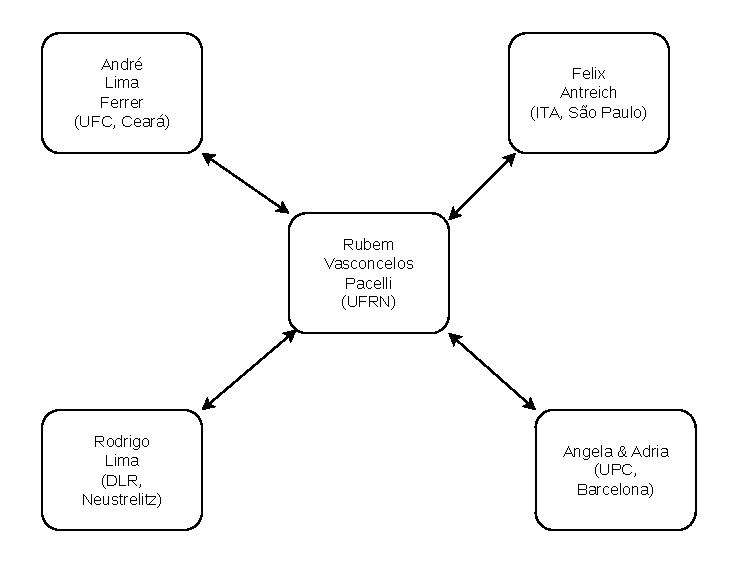
\includegraphics[width=0.85\linewidth]{Untitled Diagram.drawio.pdf}
  \caption{Diagrama de parceiros}
  \label{fig:parceiros}
\end{figure}

\subsection{Abordagem \textit{Open Science}}

Enquanto morei em São José dos Campos, São Paulo, os pesquisadores que trabalham diretamente com o prof. Felix Antreich criaram a Organização no GitHub chamada ``GPS/GNSS Laboratory (LAB-GNSS)'' \cite{felixantreichITAGPSGNSS2025}. O objetivo dessa organização hospedar dados e códigos utilizados ao decorrer das pesquisas realizadas pelo grupo de pesquisa de modo a promover a transparência, reprodutibilidade e colaboração aberta.

Acredito que essa é uma abordagem muito interessante para a pesquisa científica, e pretendo adotar essa mesma abordagem em minhas pesquisas, criando uma organização no GitHub para hospedar os dados e códigos utilizados ao decorrer das minhas pesquisas, de modo a promover a transparência, reprodutibilidade e colaboração aberta entre os colaboradores. Entendo que isso irá contribuir para a qualidade da pesquisa, para a formação de alunos de graduação e pós-graduação, e para a disseminação do conhecimento científico produzido pelo programa.

Essa metodologia está alinhada com a ideia de ciência aberta (ou \textit{open science}), que é um movimento global composto por um conjunto de princípios e práticas que busca promover um modelo de investigação mais colaborativo, transparente e acessível. Ela se baseia na premissa de disponibilizar publicações, dados de pesquisa, metodologias, softwares, códigos-fonte e recursos educacionais de forma aberta, permitindo o acesso imediato e a sua reutilização sem restrições técnicas ou legais. O objetivo central é romper com o paradigma da ciência isolada numa ``torre de marfim'', transformando o conhecimento científico num bem público e compartilhado que pertence a toda a humanidade.

A abordagem não é meramente uma questão de ética ou de acessibilidade universal, ela também é vantajosa do ponto de vista da eficiência interna do grupo de pesquisa. Um espaço virtual em que os pesquisadores compartilham seus códigos, dados, e resultados de pesquisa, pode promover a colaboração, a troca de ideias, e o desenvolvimento de projetos conjuntos. O maior benefício é a continuidade do mesmo código, realizada pelas pesquisas de outros pesquisadores que venham a ingressar no programa. Isso faz com que cada mestrado ou doutorado deixe de ser uma experiência isolada. Ao invés, cada projeto de pesquisa passa a se tornar um sistema vivo, feito por várias mãos e que evolui ao longo do tempo. Entendo que esse é o maior benefício da abordagem de ciência aberta, e é isso que pretendo promover em minhas pesquisas.

\subsection{Estação de monitoramento de sinais de rádio}

Como dito anteriormente, o desenvolvimento de uma estação de monitoramento de sinais de rádio é um dos meus objetivos de pesquisa a médio prazo. Apesar dos desafios orçamentários e de infraestrutura, acredito que esse é um projeto viável e que pode trazer muitos benefícios para o programa, para a comunidade acadêmica. A região equatorial é estratégica para a obtenção de sinais \gls{gnss} corrompidos por cintilação ionosférica, e portanto, uma estação de monitoramento de sinais de rádio no estado do Rio Grande do Norte pode contribuir para a pesquisa em cintilação ionosférica. A utilização do meu rádio definido por software, por sua vez, permitirá que sinais de cintilação sejam removidos das outras fontes. Os dados obtidos por essa estação de monitoramento podem (e devem) ser utilizados por todos do programa.

\subsection{Patentes}

Pretendo submeter patentes relacionadas às minhas pesquisas, especialmente aquelas que envolvem o desenvolvimento de novos algoritmos, técnicas ou sistemas para comunicação e navegação por satélite, processamento de sinais e imagens, e sistemas radioenlace. A proteção intelectual é uma parte importante do processo de pesquisa e desenvolvimento, e pode contribuir para a transferência de tecnologia, para a colaboração com a indústria, e para a geração de impacto social e econômico a partir das pesquisas realizadas no programa. Esse interesse contribui para a tradição de vanguarda da \gls{ufrn} em inovação tecnológica e transferência de tecnologia.

\subsection{INCT \textit{Signals} e a UFRN}

Pretendo inserir a \gls{ufrn} no seleto grupo de universidades do \gls{inct} \textit{signals}, que é um dos maiores e mais importantes institutos de pesquisa do país na área de processamento de sinais. A inserção do programa no instituto pode trazer muitos benefícios, como o acesso a recursos financeiros, a colaboração com outros pesquisadores e grupos de pesquisa, e a participação em projetos de pesquisa de grande escala. Além disso, a inserção do programa no instituto pode contribuir para a visibilidade e o reconhecimento do programa, tanto nacional quanto internacionalmente.

\subsection{Objetivos específicos alcançados com atividades de pesquisa}

Com as atividades de pesquisa, busco alcançar os objetivos específicos e1, e3, e5, e6 e e8, além de mitigar a fraqueza f2 e fortalecer a força F1, conforme descritos na Seção~\ref{sec:objetivos} e na Tabela~\ref{tab:quadro-fofa}.

\section{Atividades de extensão}

As atividades de extensão são uma parte importante da minha atuação como professor e pesquisador, pois permitem que eu contribua para a comunidade acadêmica e para a sociedade em geral. Como foi possível observar até aqui, nenhuma das ameaças descritas na Tabela~\ref{tab:quadro-fofa} foram mitigadas até o presente momento. Isso se deve ao fato de que essas questões estão fora da universidade, e é somente nas atividades de extensão que eu posso alcançá-las.

\subsection{Aumentando a complexidade industrial do Nordeste com incubação de startups de alta tecnologia}

O Nordeste é uma região que tem um grande potencial para o desenvolvimento de indústrias de alta tecnologia, mas que ainda enfrenta desafios para alcançar esse objetivo. Através das atividades de extensão, pretendo contribuir para o aumento da complexidade industrial do Nordeste, promovendo a transferência de conhecimento e tecnologia da pesquisa para as startups que a universidade abriga.

Para isso, faz-se necessário competir por programas de fomento à inovação. Atualmente, 96\% do valor da indústria de transformação no setor aeroespacial brasileiro é concentrada no estado de São Paulo \cite{investsp_setores_negocios}. Além disso, as principais agências e empresas do setor aeronáutico aeroespacial brasileiro, como \gls{inpe} e \gls{embraer}, têm suas sedes em São Paulo. Consequentemente, a maior parte dos recursos de fomento à inovação para o setor aeroespacial brasileiro é vem de São Paulo, mas é oferecido a nível nacional. A título de exemplo, o Incuba Espaço é um programa da  Agência Espacial Brasileira (AEB) desenvolvido em parceria com o Programa das Nações Unidas para o Desenvolvimento (PNUD) e o PIT - Parque de Inovação Tecnológica São José dos Campos \cite{mundogeo_incuba_espaco_2026}. O foco do Incuba Espaço é transformar dados de satélites de observação da Terra em soluções aplicadas, com potencial de virar produto, serviço ou startup. Assuntos como:
\begin{itemize}
    \item áreas irrigadas e uso de água;
    \item super-resolução de imagens de satélite;
    \item monitoramento de algas em reservatórios e hidrelétricas; e
    \item detecção de supressão de vegetação
\end{itemize}
estão entre os temas de interesse. O programa é aberto a startups de todo o país, mas a maioria das startups selecionadas são de São Paulo devido à concentração de recursos humanos e de empresas do setor aeroespacial no Vale do Paraíba.

Minha principal missão na dimensão ``extensão'', jundo à \gls{ufrn}, é trazer esse suporte de incubação, sobretudo na área espacial, para o Nordeste. Dessa forma, empresas poderão desenvolver produtos e serviços de alta tecnologia no estado do Rio Grande do Norte, gerando uma cadeia de valor local, aumentando a complexidade industrial da região, e contribuindo para o desenvolvimento econômico e social do Nordeste.

\subsection{EMBRAPII: uma experiência a ser expandida no RN}

A Figura~\ref{fig:embrapii} mostra a estrutura da \gls{embrapii} feita no \gls{lesc}, um dos prédios, que junto com o \gls{deti} e o \gls{gtel}, compõem o nicho de teleinformática\footnote{Devido à falta de normativos claros do \gls{crea}, que não reconhece ``Engenharia de Teleinformática'' como uma graduação ou área de atuação válida, a partir de 2015, este curso foi desmembrada em ``Engenharia de Telecomunicações'' e ``Engenharia de Computação'', que trabalham em conjunto no departamento de teleinformática \cite{ufc2014teleinformatica_migracao}.} da \gls{ufc}. 


\begin{figure}[H]
  \centering
  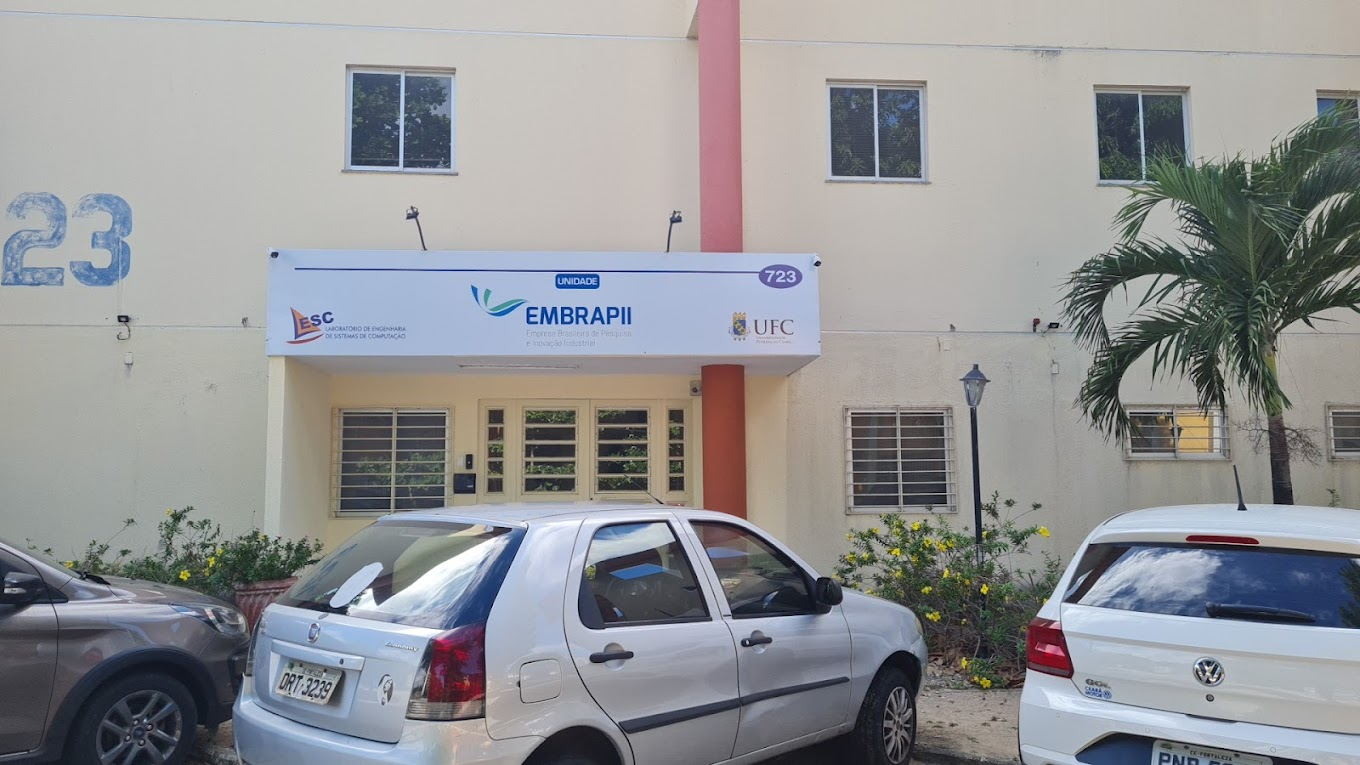
\includegraphics[width=0.85\linewidth]{embrapii.jpg}
  \caption{Estrutura da \gls{embrapii} feita no \gls{lesc} \cite{ufc2026embrapii_saude}.}
  \label{fig:embrapii}
\end{figure}

Criada recente na \gls{ufc}/\gls{lesc} \cite{ufc_embrapii_saude_2026}, a \gls{embrapii} é uma instituição de pesquisa aplicada que tem como objetivo promover a inovação tecnológica e a transferência de tecnologia entre as universidades e as empresas. A \gls{embrapii} atua em diversos setores, como aeroespacial, automotivo, energia, saúde, e outros. Através dela, as empresas podem contratar projetos de Engenharia com as universidades, com o apoio financeiro da instituição. O modelo de negócio da \gls{embrapii} une o governo federal, uma unidade executadora (também chamada de ``unidade \gls{embrapii}'') e uma empresa do setor industrial que quer desenvolver uma tecnologia de alta complexidade e de valor agregado. Cada unidade \gls{embrapii} é especializada em um setor específico e só pode contratar projetos dentro de sua área de competência. No caso do \gls{lesc}, a área de competência é em sistemas embarcados complexos, e já conseguiu atrair empresas do ramo para o estado. Juntamente com a unidade executora do \gls{ifce}, já foram realizados 102 projetos com 82 empresas de 11 unidades federativas, movimentando mais de 57 milhões de reais no estado do Ceará \cite{pimentel2022hidrogenio}.

Ao passo que incubadoras geram empresas novas, parcerias público-privada, como a que a \gls{embrapii} promove, geram atração de empresas já estabelecidas no mercado para a região em questão. Esse mecanismo de atração é a chave para combater a grande concentração de indústrias de alta tecnologia no estado de São Paulo e para promover o desenvolvimento econômico e social do Nordeste. Atualmente, a \gls{ufrn} possui uma unidade \gls{embrapii}, o \gls{imd}, especializada em internet das coisas e aplicações inteligentes em nuvem \cite{embrapii_metropole_digital_ufrn}. O que pretendo fazer é expandir a atuação da \gls{embrapii} no estado do Rio Grande do Norte, sobretudo para o setor aeronáutico, aeroespacial, focando principalmente em sistemas de telecomunicações, navegação e imageamento por satélite.

\subsection{Explorando novas parcerias no Rio Grande do Norte}

Se a região Sudeste desponta no segmento aeroespacial e aeronáutico com o estado de São Paulo, a região Nordeste desponta com o estado do Rio Grande do Norte \cite{reboucas2025ufrn_orbita_inovacao_espacial}. O estado possui parcerias estabelecidas com o \gls{inpe} de Natal, a \gls{aeb} e outros órgãos do setor aeroespacial brasileiro. Oportunidades como o \gls{crn}, \gls{cbcd}, e o \gls{conasat} oferecem oportunidades para a colaboração entre o \gls{inpe}, a \gls{ufrn}, e também com a \gls{aeb}. Um dos meus objetivos é estreitar laços com esses órgãos do setor aeroespacial, buscando oportunidades de colaboração em pesquisa, desenvolvimento de projetos conjuntos, sobretudo em:
\begin{itemize}
    \item sensoriamento remoto e observação da Terra,
    \item projeto de modems digitais a serem embarcados em CubeSats e outros tipos de satélites de pequeno porte,
    \item desenvolvimento de algoritmos de processamento de sinais e imagens,
\end{itemize}

Devido ao meu \textit{background}, acredito que posso atuar tanto no sistema de comunicação da carga útil quanto no módulo de telemetria, rastreamento e controle (TT\&C) de nanossatélites. Concomitantemente, também posso atuar diretamente nos dados provenientes de satélites, processando-os a fim de extrair informações relevantes para a aplicação em específico.

A colaboração com o \gls{inpe} pode trazer muitos benefícios para o programa, como o acesso a recursos financeiros, a participação em projetos de pesquisa de grande escala, e a oportunidade de trabalhar com pesquisadores de renome na área de sensoriamento remoto e observação da Terra.

\subsection{Objetivos específicos alcançados com atividades de extensão}

Com as atividades de extensão, busco alcançar os objetivos específicos e2, e3, e e4, além de mitigar as ameaças A1 e A2 e fortalecer a oportunidade O1, conforme descritos na Seção~\ref{sec:objetivos} e na Tabela~\ref{tab:quadro-fofa}.

\section{Metas a curto, médio e longo prazo}

As metas propostas foram organizadas em horizontes de curto, médio e longo
prazo, considerando a necessidade de inserção institucional gradual,
consolidação de linhas de atuação e desenvolvimento de atividades de ensino,
pesquisa, extensão e inovação.

\begin{itemize}
  \item \textbf{Curto prazo: primeiro e segundo anos}
  \begin{itemize}
    \item Integrar-se às atividades acadêmicas do departamento, contribuindo
    com disciplinas relacionadas a telecomunicações, processamento digital de
    sinais, comunicações digitais, sistemas aeroespaciais, inteligência
    artificial aplicada à engenharia e áreas correlatas;

    \item Estruturar materiais didáticos, roteiros de simulação e atividades
    práticas baseadas em ferramentas computacionais, tais como MATLAB, Python, Julia, GNU Radio, GNU/Linux,
    ambientes de simulação para circuitos eletrônicos, sistemas computacionais embarcados, e plataformas de rádio definido por software,;

    \item Iniciar a orientação de estudantes de graduação, por meio de trabalhos
    de conclusão de curso, iniciação científica e projetos de desenvolvimento
    tecnológico;

    \item Submeter ao menos um projeto de pesquisa ou extensão a editais
    institucionais ou agências de fomento, buscando viabilizar a criação de uma
    linha de atuação em telecomunicações, processamento de sinais, inteligência
    artificial e sistemas espaciais;

    \item Publicar ou submeter ao menos um artigo científico em periódico ou
    congresso especializado, preferencialmente a partir da continuidade das
    pesquisas já desenvolvidas e de novas colaborações institucionais.
  \end{itemize}

  \item \textbf{Médio prazo: terceiro e quarto anos}
  \begin{itemize}
    \item Consolidar uma linha de pesquisa em processamento estatístico de
    sinais, aprendizagem de máquina aplicada a séries temporais, comunicações
    digitais, sistemas de navegação por satélite, monitoramento ionosférico e
    sistemas aeroespaciais;

    \item Ampliar a orientação de estudantes de graduação e, quando possível,
    de pós-graduação, vinculando suas atividades a projetos de pesquisa,
    inovação e extensão tecnológica;

    \item Submeter projetos de maior porte a agências de fomento estaduais e
    nacionais, bem como buscar parcerias com instituições públicas, empresas,
    incubadoras, parques tecnológicos e ambientes de inovação;

    \item Estabelecer uma estação de monitoramento de cintilação ionosférica para
    caracterização de distúrbios ionosféricos e suas implicações em sistemas de
    navegação e telecomunicações via satélite, especialmente na região equatorial;

    \item Manter produção científica regular, com submissão de artigos em periódicos e congressos nacionais e internacionais nas áreas de telecomunicações, processamento de sinais, inteligência
    artificial e sistemas espaciais.
  \end{itemize}

  \item \textbf{Longo prazo: a partir do quinto ano}
  \begin{itemize}
    \item Contribuir para a consolidação de um núcleo ou linha institucional de
    pesquisa em telecomunicações, processamento de sinais, inteligência
    artificial aplicada à engenharia e sistemas aeroespaciais;

    \item Fortalecer redes de colaboração nacional e internacional, envolvendo
    universidades, institutos de pesquisa, empresas e centros tecnológicos;

    \item Captar recursos para infraestrutura laboratorial, bolsas de pesquisa,
    equipamentos, softwares e plataformas experimentais voltadas ao ensino e à
    pesquisa aplicada;

    \item Formar recursos humanos qualificados para atuação acadêmica,
    científica, tecnológica e industrial, especialmente em áreas estratégicas
    para o desenvolvimento regional e nacional;

    \item Gerar desdobramentos científicos e tecnológicos, incluindo publicações,
    produtos técnicos, softwares, protótipos, propriedade intelectual e ações de
    transferência de conhecimento para a sociedade e o setor produtivo.
  \end{itemize}
\end{itemize}

\section{Conclusão}

Espera-se que, com a implementação das atividades de ensino, pesquisa e extensão descritas neste plano de trabalho, seja possível alcançar o objetivo geral de contribuir para o desenvolvimento do \gls{ppgeec} da \gls{ufrn}, promovendo a excelência acadêmica, a produção científica de qualidade, a formação de recursos humanos qualificados, e a transferência de conhecimento e tecnologia para a sociedade. A integração entre as atividades de ensino, pesquisa e extensão é fundamental para o sucesso do plano de trabalho, e para a construção de um ambiente acadêmico dinâmico, colaborativo e inovador.

% Ensure all glossary entries are included in the printed glossaries,
% even if some were not referenced in the document.
\printglossaries % to print the glossary, add `automake` as the fist option in the `glossaries-extra` pkg import (see the `default_preamble.tex` file)
\printbibliography
\end{document}
